% ******************************* PhD Thesis Template **************************
% Please have a look at the README.md file for info on how to use the template

\documentclass[a4paper,12pt,times,numbered,print,index,draft]{Classes/PhDThesisPSnPDF}

% ******************************************************************************
% ******************************* Class Options ********************************
% *********************** See README for more details **************************
% ******************************************************************************

% `a4paper'(The University of Cambridge PhD thesis guidelines recommends a page
% size a4 - default option) or `a5paper': A5 Paper size is also allowed as per
% the Cambridge University Engineering Deparment guidelines for PhD thesis
%
% `11pt' or `12pt'(default): Font Size 10pt is NOT recommended by the University
% guidelines
%
% `oneside' or `twoside'(default): Printing double side (twoside) or single
% side.
%
% `print': Use `print' for print version with appropriate margins and page
% layout. Leaving the options field blank will activate Online version.
%
% `index': For index at the end of the thesis
%
% `draftclassic': For draft mode without loading any images (same as draft in book)
%
% `draft': Special draft mode with line numbers, images, and water mark with
% timestamp and custom text. Position of the text can also be modified.
%
% `abstract': To generate only the title page and abstract page with
% dissertation title and name, to submit to the Student Registry
%
% `chapter`: This option enables only the specified chapter and it's references
%  Useful for review and corrections.
%
% ************************* Custom Page Margins ********************************
%
% `custommargin`: Use `custommargin' in options to activate custom page margins,
% which can be defined in the preamble.tex. Custom margin will override
% print/online margin setup.
%
% *********************** Choosing the Fonts in Class Options ******************
%
% `times' : Times font with math support. (The Cambridge University guidelines
% recommend using times)
%
% `fourier': Utopia Font with Fourier Math font (Font has to be installed)
%            It's a free font.
%
% `customfont': Use `customfont' option in the document class and load the
% package in the preamble.tex
%
% default or leave empty: `Latin Modern' font will be loaded.
%
% ********************** Choosing the Bibliography style ***********************
%
% `authoryear': For author-year citation eg., Krishna (2013)
%
% `numbered': (Default Option) For numbered and sorted citation e.g., [1,5,2]
%
% `custombib': Define your own bibliography style in the `preamble.tex' file.
%              `\RequirePackage[square, sort, numbers, authoryear]{natbib}'.
%              This can be also used to load biblatex instead of natbib
%              (See Preamble)
%
% **************************** Choosing the Page Style *************************
%
% `default (leave empty)': For Page Numbers in Header (Left Even, Right Odd) and
% Chapter Name in Header (Right Even) and Section Name (Left Odd). Blank Footer.
%
% `PageStyleI': Chapter Name next & Page Number on Even Side (Left Even).
% Section Name & Page Number in Header on Odd Side (Right Odd). Footer is empty.
%
% `PageStyleII': Chapter Name on Even Side (Left Even) in Header. Section Number
% and Section Name in Header on Odd Side (Right Odd). Page numbering in footer


% ********************************** Preamble **********************************
% Preamble: Contains packages and user-defined commands and settings
% ******************************************************************************
% ****************************** Custom Margin *********************************

% Add `custommargin' in the document class options to use this section
% Set {innerside margin / outerside margin / topmargin / bottom margin}  and
% other page dimensions
\ifsetCustomMargin
  \RequirePackage[left=37mm,right=30mm,top=35mm,bottom=30mm]{geometry}
  \setFancyHdr % To apply fancy header after geometry package is loaded
\fi

% Add spaces between paragraphs
%\setlength{\parskip}{0.5em}
% Ragged bottom avoids extra whitespaces between paragraphs
\raggedbottom
% To remove the excess top spacing for enumeration, list and description
%\usepackage{enumitem}
%\setlist[enumerate,itemize,description]{topsep=0em}

% *****************************************************************************
% ******************* Fonts (like different typewriter fonts etc.)*************

% Add `customfont' in the document class option to use this section

\ifsetCustomFont
  % Set your custom font here and use `customfont' in options. Leave empty to
  % load computer modern font (default LaTeX font).
  %\RequirePackage{helvet}

  % For use with XeLaTeX
  %  \setmainfont[
  %    Path              = ./libertine/opentype/,
  %    Extension         = .otf,
  %    UprightFont = LinLibertine_R,
  %    BoldFont = LinLibertine_RZ, % Linux Libertine O Regular Semibold
  %    ItalicFont = LinLibertine_RI,
  %    BoldItalicFont = LinLibertine_RZI, % Linux Libertine O Regular Semibold Italic
  %  ]
  %  {libertine}
  %  % load font from system font
  %  \newfontfamily\libertinesystemfont{Linux Libertine O}
\fi

% *****************************************************************************
% **************************** Custom Packages ********************************

% ************************* Algorithms and Pseudocode **************************

%\usepackage{algpseudocode}


% ********************Captions and Hyperreferencing / URL **********************

% Captions: This makes captions of figures use a boldfaced small font.
%\RequirePackage[small,bf]{caption}

\RequirePackage[labelsep=space,tableposition=top]{caption}
\renewcommand{\figurename}{Fig.} %to support older versions of captions.sty


% *************************** Graphics and figures *****************************

%\usepackage{rotating}
%\usepackage{wrapfig}

% Uncomment the following two lines to force Latex to place the figure.
% Use [H] when including graphics. Note 'H' instead of 'h'
%\usepackage{float}
%\restylefloat{figure}

% Subcaption package is also available in the sty folder you can use that by
% uncommenting the following line
% This is for people stuck with older versions of texlive
%\usepackage{sty/caption/subcaption}
\usepackage{subcaption}

% ********************************** Tables ************************************
\usepackage{booktabs} % For professional looking tables
\usepackage{multirow}

%\usepackage{multicol}
%\usepackage{longtable}
%\usepackage{tabularx}


% *********************************** SI Units *********************************
\usepackage{siunitx} % use this package module for SI units


% ******************************* Line Spacing *********************************

% Choose linespacing as appropriate. Default is one-half line spacing as per the
% University guidelines

% \doublespacing
% \onehalfspacing
% \singlespacing


% ************************ Formatting / Footnote *******************************

% Don't break enumeration (etc.) across pages in an ugly manner (default 10000)
%\clubpenalty=500
%\widowpenalty=500

%\usepackage[perpage]{footmisc} %Range of footnote options


% *****************************************************************************
% *************************** Bibliography  and References ********************

%\usepackage{cleveref} %Referencing without need to explicitly state fig /table

% Add `custombib' in the document class option to use this section
\ifuseCustomBib
   \RequirePackage[square, sort, numbers, authoryear]{natbib} % CustomBib

% If you would like to use biblatex for your reference management, as opposed to the default `natbibpackage` pass the option `custombib` in the document class. Comment out the previous line to make sure you don't load the natbib package. Uncomment the following lines and specify the location of references.bib file

%\RequirePackage[backend=biber, style=numeric-comp, citestyle=numeric, sorting=nty, natbib=true]{biblatex}
%\bibliography{References/references} %Location of references.bib only for biblatex

\fi

% changes the default name `Bibliography` -> `References'
\renewcommand{\bibname}{References}


% ******************************** Roman Pages *********************************
% The romanpages environment set the page numbering to lowercase roman one
% for the contents and figures lists. It also resets
% page-numbering for the remainder of the dissertation (arabic, starting at 1).

\newenvironment{romanpages}{
  \setcounter{page}{1}
  \renewcommand{\thepage}{\roman{page}}}
{\newpage\renewcommand{\thepage}{\arabic{page}}}


% ******************************************************************************
% ************************* User Defined Commands ******************************
% ******************************************************************************

% *********** To change the name of Table of Contents / LOF and LOT ************

%\renewcommand{\contentsname}{My Table of Contents}
%\renewcommand{\listfigurename}{My List of Figures}
%\renewcommand{\listtablename}{My List of Tables}


% ********************** TOC depth and numbering depth *************************

\setcounter{secnumdepth}{2}
\setcounter{tocdepth}{2}


% ******************************* Nomenclature *********************************

% To change the name of the Nomenclature section, uncomment the following line

%\renewcommand{\nomname}{Symbols}


% ********************************* Appendix ***********************************

% The default value of both \appendixtocname and \appendixpagename is `Appendices'. These names can all be changed via:

%\renewcommand{\appendixtocname}{List of appendices}
%\renewcommand{\appendixname}{Appndx}

% *********************** Configure Draft Mode **********************************

% Uncomment to disable figures in `draftmode'
%\setkeys{Gin}{draft=true}  % set draft to false to enable figures in `draft'

% These options are active only during the draft mode
% Default text is "Draft"
%\SetDraftText{DRAFT}

% Default Watermark location is top. Location (top/bottom)
%\SetDraftWMPosition{bottom}

% Draft Version - default is v1.0
%\SetDraftVersion{v1.1}

% Draft Text grayscale value (should be between 0-black and 1-white)
% Default value is 0.75
%\SetDraftGrayScale{0.8}


% ******************************** Todo Notes **********************************
%% Uncomment the following lines to have todonotes.

\ifsetDraft
	\usepackage[colorinlistoftodos]{todonotes}
	\newcommand{\mynote}[1]{\todo[author=Wojtek,size=\small,inline,color=green!40]{#1}}
\else
	\newcommand{\mynote}[1]{}
	\newcommand{\listoftodos}{}
\fi

% Example todo: \mynote{Hey! I have a note}


% ************************ Thesis Information & Meta-data **********************
% Thesis title and author information, refernce file for biblatex
% ************************ Thesis Information & Meta-data **********************
%% The title of the thesis
\title{Competition between Weak Quantum Measurement and Many-Body
Dynamics in Ultracold Bosonic Gases}
%\texorpdfstring is used for PDF metadata. Usage:
%\texorpdfstring{LaTeX_Version}{PDF Version (non-latex)} eg.,
%\texorpdfstring{$sigma$}{sigma}

%% Subtitle (Optional)
%\subtitle{Using the CUED template}

%% The full name of the author
\author{Wojciech Kozlowski}

%% Department (eg. Department of Engineering, Maths, Physics)
\dept{Department of Physics}

%% University and Crest
\university{University of Oxford}
% Crest minimum should be 30mm.
\crest{
\includegraphics[width=0.2\textwidth]{University_Crest}}
%% Use this crest, if you are using the college crest
%% Crest long miminum should be 65mm
%\crest{
\includegraphics[width=0.45\textwidth]{University_Crest_Long}}

%% College shield [optional] 
% Crest minimum should be 30mm.
%\collegeshield{
\includegraphics[width=0.2\textwidth]{CollegeShields/Kings}}


%% Supervisor (optional)
\supervisor{Dr. Igor B. Mekhov}
%% Supervisor Role (optional) - Supervisor (default) or advisor
%\supervisorrole{Advisor: }

%% Advisor (optional)
%\advisor{Prof. Malcolm Bolton}
%% Advisor Role (optional) - Advisor (default) or leave empty
%\advisorrole{Advisor: }


%% You can redefine the submission text:
% Default as per the University guidelines:
% ``This dissertation is submitted for the degree of''
%\renewcommand{\submissiontext}{change the default text here if needed}

%% Full title of the Degree
\degreetitle{Doctor of Philosophy}

%% College affiliation (optional)
\college{St. Catherine's College}

%% Submission date
% Default is set as {\monthname[\the\month]\space\the\year}
%\degreedate{September 2014} 

%% Meta information
%\subject{LaTeX} \keywords{{LaTeX} {PhD Thesis} {Engineering} {University of
%Cambridge}}


% ***************************** Abstract Separate ******************************
% To printout only the titlepage and the abstract with the PhD title and the
% author name for submission to the Student Registry, use the `abstract' option in
% the document class.

\ifdefineAbstract
 \pagestyle{empty}
 \includeonly{Declaration/declaration, Abstract/abstract}
\fi

% ***************************** Chapter Mode ***********************************
% The chapter mode allows user to only print particular chapters with references
% Title, Contents, Frontmatter are disabled by default
% Useful option to review a particular chapter or to send it to supervisior.
% To use choose `chapter' option in the document class

\ifdefineChapter
 \includeonly{Chapter3/chapter3}
\fi

% ******************************** Front Matter ********************************
\begin{document}

\frontmatter

\begin{titlepage}
  \maketitle
\end{titlepage}


% ******************************* Thesis Dedidcation ********************************

\begin{dedication} 

\emph{Moim rodzicom, bez których nie byłbym w stanie osiągnąć tego
  wszystkiego.}

\emph{To my parents without whom I would not have been able to achieve
  any of this.}
  
\end{dedication}


% ******************************* Thesis Declaration ***************************

\begin{declaration}

\mynote{Do I need this? Is there an Oxford University version?}

I hereby declare that except where specific reference is made to the work of 
others, the contents of this dissertation are original and have not been 
submitted in whole or in part for consideration for any other degree or 
qualification in this, or any other university. This dissertation is my own 
work and contains nothing which is the outcome of work done in collaboration 
with others, except as specified in the text and Acknowledgements. This 
dissertation contains fewer than 65,000 words including appendices, 
bibliography, footnotes, tables and equations and has fewer than 150 figures.

% Author and date will be inserted automatically from thesis.tex \author \degreedate

\end{declaration}


% ************************** Thesis Acknowledgements **************************

\begin{acknowledgements}      

First and foremost, I would like to thank my supervisor Dr. Igor
Mekhov who has been an excellent mentor throughout my time at
Oxford. It is primarily thanks to his brilliant insights and
professionalism that I was able to reach my full potential during my
doctoral studies. The work contained in this thesis would also not be
possible without the help of the other members of the group, Gabriel
Mazzucchi and Dr. Santiago Caballero-Benitez. Without our frequent
casual discussions in the Old Library office I would have still been
stuck on the third chapter. I would also like to acknowledge all
members of Prof. Dieter Jaksch's and Prof. Christopher Foot's groups
for various helpful discussions. I must also offer a special mention
for Edward Owen who provided much needed reality checks on some of my
wishful theoretical thinking. I would also like to express my
gratitude to EPSRC, St. Catherine's College, the ALP sub-department,
and the Institute of Physics for providing me with the financial means
to live and study in Oxford as well as attend several conferences in
the UK and abroad.

On a personal note, I would like to thank my parents who provided me
with all the skills necessary work towards any goals I set
myself. Needless to say, without them I would have never been able to
be where I am right now. I would like to thank all the new and old
friends that have kept me company for the last four years. The time
spent together provided a welcome respite from the sweat and toil of
my DPhil.

\vspace{2em}
\raggedleft{Oxford, September 2016}

\end{acknowledgements}

% ************************** Thesis Abstract *****************************
% Use `abstract' as an option in the document class to print only the titlepage and the abstract.
\begin{abstract}
  Trapping ultracold atoms in optical lattices enabled the study of
  strongly correlated phenomena in an environment that is far more
  controllable and tunable than what was possible in condensed
  matter. Here, we consider coupling these systems to quantized light
  where the quantum nature of both the optical and matter fields play
  equally important roles in order to push the boundaries of
  what is possible in ultracold atomic systems.

  We show that light can serve as a nondestructive probe of the
  quantum state of the matter. By condering a global
  measurement scheme we show that it is possible to distinguish a
  highly delocalised phase like a superfluid from insulators. We also
  demonstrate that light scattering reveals not only density
  correlations, but also matter-field interference.

  By taking into account the effect of measurement backaction we show
  that the measurement can efficiently compete with the local atomic
  dynamics of the quantum gas. This can generate long-range
  correlations and entanglement which in turn leads to macroscopic
  multimode oscillations accross the whole lattice when the
  measurement is weak and correlated tunneling, as well as selective
  suppression and enhancement of dynamical processes beyond the
  projective limit of the quantum Zeno effect in the strong
  measurement regime. 

  We also consider quantum measurement backaction due to the
  measurement of matter-phase-related variables such as global phase
  coherence. We show how this unconventional approach opens up new
  opportunities to affect system evolution and demonstrate how this
  can lead to a new class of measurement projections, thus extending
  the measurement postulate for the case of strong competition with
  the system’s own evolution.
\end{abstract}


% *********************** Adding TOC and List of Figures ***********************

\tableofcontents

\listoffigures

\listoftables

% \printnomenclature[space] space can be set as 2em between symbol and description
%\printnomenclature[3em]

\printnomenclature

% ******************************** Main Matter *********************************
\mainmatter

%*******************************************************************************
%*********************************** First Chapter *****************************
%*******************************************************************************

\chapter{Introduction}  %Title of the First Chapter

\ifpdf
    \graphicspath{{Chapter1/Figs/Raster/}{Chapter1/Figs/PDF/}{Chapter1/Figs/}}
\else
    \graphicspath{{Chapter1/Figs/Vector/}{Chapter1/Figs/}}
\fi


The field of ultracold gases has been a rapidly growing field ever
since the first Bose-Einstein condensate (BEC) was obtained in 1995
\cite{anderson1995, bradley1995, davis1995}. This new quantum state of
matter is characterised by a macroscopic occupancy of the single
particle ground state at which point the whole system behaves like a
single many-body quantum object \cite{PitaevskiiStringari}. This was
revolutionary as it enabled the study of coherent properties of
macroscopic systems rather than single atoms or photons. Furthermore,
the advanced state of laser cooling and manipulation technologies
meant that the degree of control and isolation from the environment
was far greater than was possible in condensed matter systems
\cite{lewenstein2007, bloch2008}. Initially, the main focus of the
research was on the properties of coherent matter waves, such as
interference properties \cite{andrews1997}, long range phase coherence
\cite{bloch2000}, or quantised vortices \cite{matthews1999,
  madison2000, abo2001}. Fermi degeneracy in ultracold gases was
obtained shortly afterwards opening a similar field for fermions
\cite{demarco1999, schreck2001, truscott2001}.

In 1998 it was shown that a degenerate ultracold gas trapped in an
optical lattice is a near-perfect realisation of the Bose-Hubbard
model \cite{jaksch1998} and in 2002 it was already demonstrated in a
ground-breaking experiment \cite{greiner2002}. The Bose-Hubbard
Hamiltonian was previously known in the field of condensed matter
where it was considered a simple toy model. Despite its simplicity the
model exhibits a variety of different interesting phenomena such as
the quantum phase transition from a delocalised superfluid state to a
Mott insulator as the on-site interaction is increased above a
critical point which was originally studied in the context of liquid
helium \cite{fisher1989}. In contrast to a thermodynamic phase
transition, a quantum phase transition is driven by quantum
fluctuations and can occur at zero temperature. The ability to achieve
a Bose-Hubbard Hamiltonian where the model parameters can be easily
tuned by varying the lattice potential opened up a new regime in the
many-body physics of atomic gases. Unlike Bose-Einstein condensates in
free space which are described by weakly interacting theories
\cite{dalfovo1999}, the behaviour of ultracold gases trapped in an
optical lattice is dominated by atomic interactions opening the
possibility of studying strongly correlated behaviour with
unprecendented control.

The modern field of ultracold gases is successful due to its
interdisciplinarity \cite{lewenstein2007, bloch2008}. Originally
condensed matter effects are now mimicked in controlled atomic systems
finding applications in areas such as quantum information
processing. A really new challenge is to identify novel phenomena
which were unreasonable to consider in condensed matter, but will
become feasible in new systems. One such direction is merging quantum
optics and many-body physics \cite{mekhov2012, ritsch2013}. Quantum
optics has been developping as a branch of quantum physics
independently of the progress in the many-body community. It describes
delicate effects such as quantum measurement, state engineering, and
systems that can generally be easily isolated from their environnment
due to the non-interacting nature of photons \cite{Scully}. However,
they are also the perfect candidate for studying open systems due the
advanced state of cavity technologies \cite{carmichael,
  MeasurementControl}. On the other hand ultracold gases are now used
to study strongly correlated behaviour of complex macroscopic
ensembles where decoherence is not so easy to avoid or control. Recent
experimental progress in combining the two fields offered a very
promising candidate for taking many-body physics in a direction that
would not be possible for condensed matter \cite{baumann2010,
  wolke2012, schmidt2014}. Two very recent breakthrough experiments
have even managed to couple an ultracold gas trapped in an optical
lattice to an optical cavity enabling the study of strongly correlated
systems coupled to quantized light fields where the quantum properties
of the atoms become imprinted in the scattered light
\cite{klinder2015, landig2016}.

There are three prominent directions in which the field of quantum
optics of quantum gases has progressed in. First, the use of quantised
light enables direct coupling to the quantum properties of the atoms
\cite{mekhov2007prl, mekhov2007prl, mekhov2012}. This allows us to
probe the many-body system in a nondestructive manner and under
certain conditions even perform quantum non-demolition (QND)
measurements. QND measurements were originally developed in the
context of quantum optics as a tool to measure a quantum system
without significantly disturbing it \cite{braginsky1977, unruh1978,
  brune1990, brune1992}. This has naturally been extended into the
realm of ultracold gases where such non-demolition schemes have been
applied to both fermionic \cite{eckert2008qnd, roscilde2009} and
bosonic \cite{hauke2013, rogers2014}. In this thesis, we consider
light scattering in free space from a bosonic ultracold gas and show
that there are many prominent features that go beyond classical
optics. Even the scattering angular distribution is nontrivial with
Bragg conditions that are significantly different from the classical
case. Furthermore, we show that the direct coupling of quantised light
to the atomic systems enables the nondestructive probing beyond a
standard mean-field description. We demonstrate this by showing that
the whole phase diagram of a disordered one-dimensional Bose-Hubbard
Hamiltonian, which consists of the superfluid, Mott insulating, and
Bose glass phases, can be mapped from the properties of the scattered
light. Additionally, we go beyond standard QND approaches, which only
consider coupling to density observables, by also considering the
direct coupling of the quantised light to the interference between
neighbouring lattice sites. We show that not only is this possible to
achieve in a nondestructive manner, it is also achieved without the
need for single-site resolution. This is in contrast to the standard
destructive time-of-flight measurements currently used to perform
these measurements \cite{miyake2011}. Within a mean-field treatment
this enables probing of the order parameter as well as matter-field
quadratures and their squeezing. This can have an impact on atom-wave
metrology and information processing in areas where quantum optics has
already made progress, e.g.,~quantum imaging with pixellized sources
of non-classical light \cite{golubev2010, kolobov1999}, as an optical
lattice is a natural source of multimode nonclassical matter waves.

Second, coupling a quantum gas to a cavity also enables us to study
open system many-body dynamics either via dissipation where we have no
control over the coupling to the environment or via controlled state
reduction using the measurement backaction due to photodetections. A
lot of effort was expanded in an attempt to minimise the influence of
the environment in order to extend decoherence times. However,
theoretical progress in the field has shown that instead being an
obstacle, dissipation can actually be used as a tool in engineering
quantum states \cite{diehl2008}. Furthermore, as the environment
coupling is varied the system may exhibit sudden changes in the
properties of its steady state giving rise to dissipative phase
transitions \cite{carmichael1980, werner2005, capriotti2005,
  morrison2008, eisert2010, bhaseen2012, diehl2010,
  vznidarivc2011}. An alternative approach to open systems is to look
at quantum measurement where we consider a quantum state conditioned
on the outcome of a single experimental run \cite{carmichael,
  MeasurementControl}. In this approach we consider the solutions to a
stochastic Schr\"{o}dinger equation which will be a pure state, which
in contrast to dissipative systems is generally not the case. The
question of measurement and its effect on the quantum state has been
around since the inception of quantum theory and still remains a
largely open question \cite{zurek2002}. It wasn't long after the first
condenste was obtained that theoretical work on the effects of
measurement on BECs appeared \cite{cirac1996, castin1997,
  ruostekoski1997}. Recently, work has also begun on combining weak
measurement with the strongly correlated dynamics of ultracold gases
in optical lattices \cite{mekhov2009prl, mekhov2009pra, mekhov2012,
  douglas2012, douglas2013, ashida2015, ashida2015a}.

In this thesis we focus on the latter by considering a quantum gas in
an optical lattice coupled to a cavity \cite{mekhov2012}. This
provides us with a flexible setup where the global light scattering
can be engineered. We show that this introduces a new competing energy
scale into the system and by considering continuous measurement, as
opposed to discrete projective measurements, we demonstrate the
quantum backaction can effectively compete with the standard
short-range processes of the Bose-Hubbard model. The global nature of
the optical fields leads to new phenomena driven by long-range
correlations that arise from the measurement. The flexibility of the
optical setup lets us not only consider coupling to different
observables, but by carefully choosing the optical geometry we can
suppress or enhace specific dynamical processes, realising spatially
nonlocal quantum Zeno dynamics.

The quantum Zeno effect happens when frequent measurements slow the
evolution of a quantum system \cite{misra1977, facchi2008}. This
effect was already considered by von Neumann and it has been
successfully observed in a variety of systems \cite{itano1990,
  nagels1997, kwiat1999, balzer2000, streed2006, hosten2006,
  bernu2008}. The generalisation of this effect to measurements with
multidimensional projections leads to quantum Zeno dynamics where
unitary evolution is uninhibited within this degenerate subspace,
i.e. the Zeno subspace \cite{facchi2008, raimond2010, raimond2012,
  signoles2014}. Here, by combining quantum optical measurements with
the complex Hilbert space of a many-body quantum gas we go beyond
conventional quantum Zeno dynamics. By considering the case of
measurement near, but not in, the projective limit the system is still
confined to a Zeno subspace, but intermediate transitions are allowed
via virtual Raman-like processes. In a lattice system, like the
Bose-Hubbard model we can use global measurement to engineer these
dynamics to be highly nonlocal leading to the generation of long-range
correlations and entanglement. Furthermore, we show that this
behaviour can be approximated by a non-Hermitian Hamiltonian thus
extending the notion of quantum Zeno dynamics into the realm of
non-Hermitian quantum mechanics joining the two
paradigms. Non-Hermitian systems themself exhibit a range of
interesting phenomena ranging from localisation \cite{hatano1996,
  refael2006} and $\mathcal{PT}$ symmetry \cite{bender1998,
  giorgi2010, zhang2013} to spatial order \cite{otterbach2014} and
novel phase transitions \cite{lee2014prx, lee2014prl}.

Just like for the nondestructive measurements we also consider
measurement backaction due to coupling to the interference terms
between the lattice sites. This effectively amounts to coupling to the
phase observables of the system. As this is the conjugate variable of
density, this allows to enter a new regime of quantum control using
measurement backaction. Whilst such interference measurements have
been previously proposed for BECs in double-wells \cite{cirac1996,
  castin1997, ruostekoski1997}, the extension to a lattice system is
not straightforward, but we will show it is possible to achieve with
our propsed setup by a careful optical arrangement. Within this
context we demonstrate a novel type of projection which occurs even
when there is significant competition with the Hamiltonian
dynamics. This projection is fundamentally different to the standard
formulation of the Copenhagen postulate projection or the quantum Zeno
effect \cite{misra1977, facchi2008} thus providing an extension of the
measurement postulate to dynamical systems subject to weak
measurement.

Finally, the cavity field that builds up from the scattered photons
can also create a quantum optical potential which will modify the
Hamiltonian in a way that depends on the state of the atoms that
scatterd the light. This can lead to new quantum phases due to new
types of long-range interactions being mediated by the global quantum
optical fields \cite{caballero2015, caballero2015njp, caballero2016,
  caballero2016a}. However, this aspect of quantum optics of quantum
gases is beyond the scope of this thesis.

%*******************************************************************************
%*********************************** Second Chapter ****************************
%*******************************************************************************

%Title of the Second Chapter
\chapter{Quantum Optics of Quantum Gases}  

\ifpdf
    \graphicspath{{Chapter2/Figs/Raster/}{Chapter2/Figs/PDF/}{Chapter2/Figs/}}
\else
    \graphicspath{{Chapter2/Figs/Vector/}{Chapter2/Figs/}}
\fi


%********************************** % First Section  ****************************

\section{Ultracold Atoms in Optical Lattices}

%********************************** % Second Section  ***************************

\section{Quantum Optics of Quantum Gases}

Having introduced and described the behaviour of ultracold bosons
trapped and manipulated using classical light, it is time to extend
the discussion to quantized optical fields. We will first derive a
general Hamiltonian that describes the coupling of atoms with
far-detuned optical beams \cite{mekhov2012}. This will serve as the
basis from which we explore the system in different parameter regimes,
such as nondestructive measurement in free space or quantum
measurement backaction in a cavity.

We consider $N$ two-level atoms in an optical lattice with $M$
sites. For simplicity we will restrict our attention to spinless
bosons, although it is straightforward to generalise to fermions,
which yields its own set of interesting quantum phenomena
\cite{atoms2015, mazzucchi2016, mazzucchi2016af}, and other spin
particles. The theory can be also be generalised to continuous
systems, but the restriction to optical lattices is convenient for a
variety of reasons. Firstly, it allows us to precisely describe a
many-body atomic state over a broad range of parameter values due to
the inherent tunability of such lattices. Furthermore, this model is
capable of describing a range of different experimental setups ranging
from a small number of sites with a large filling factor (e.g.~BECs
trapped in a double-well potential) to a an extended multi-site
lattice with a low filling factor (e.g.~a system with one atom per
site will exhibit the Mott insulator to superfluid quantum phase
transition). \mynote{extra fermion citations, Piazza? Look up Gabi's
  AF paper.}

\mynote{Potentially some more crap, but come to think of it the
  content will strongly depend on what was included in the preceding
  section on plain ultracold bosons}

As we have seen in the previous section, an optical lattice can be
formed with classical light beams that form standing waves. Depending
on the detuning with respect to the atomic resonance, the nodes or
antinodes form the lattice sites in which atoms accumulate. As shown
in Fig. \ref{fig:LatticeDiagram} the trapped bosons (green) are
illuminated with a coherent probe beam (red) and scatter light into a
different mode (blue) which is then measured with a detector. The most
straightforward measurement is to simply count the number of photons
with a photodetector, but it is also possible to perform a quadrature
measurement by using a homodyne detection scheme. The experiment can
be performed in free space where light can scatter in any
direction. The atoms can also be placed inside a cavity which has the
advantage of being able to enhance light scattering in a particular
direction. Furthermore, cavities allow for the formation of a fully
quantum potential in contrast to the classical lattice trap.

\begin{figure}[htbp!]
  \centering
  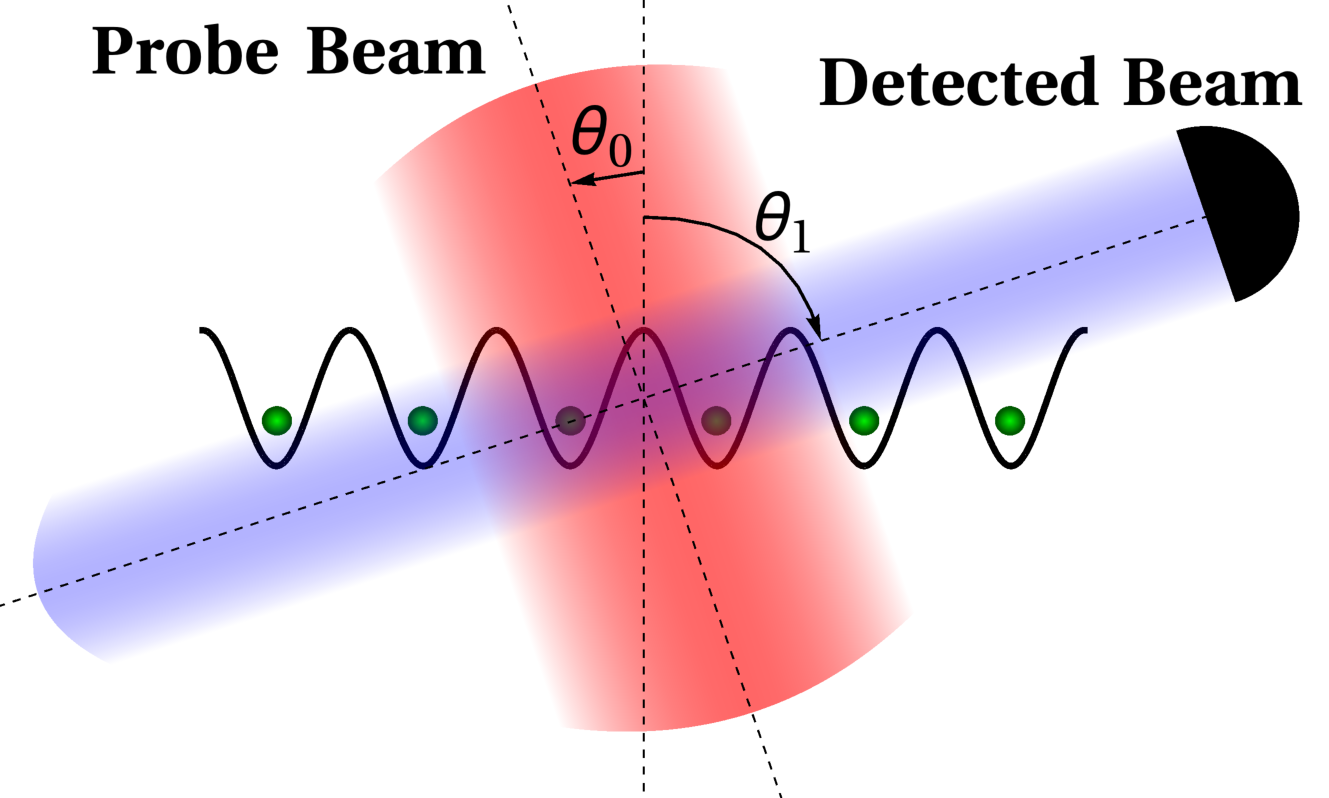
\includegraphics[width=1.0\textwidth]{LatticeDiagram}
  \caption[Experimental Setup]{Atoms (green) trapped in an optical
    lattice are illuminated by a coherent probe beam (red). The light
    scatters (blue) in free space or into a cavity and is measured by
    a detector. If the experiment is in free space light can scatter
    in any direction. A cavity on the other hand enhances scattering
    in one particular direction.}
  \label{fig:LatticeDiagram}
\end{figure}

For simplicity, we will be considering one-dimensional lattices most
of the time. However, the model itself is derived for any number of
dimensions and since none of our arguments will ever rely on
dimensionality our results straightforwardly generalise to 2- and 3-D
systems. This simplification allows us to present a much simpler
picture of the physical setup where we only need to concern ourselves
with a single angle for each optical mode. As shown in
Fig. \ref{fig:LatticeDiagram} the angle between the normal to the
lattice and the probe and detected beam are denoted by $\theta_0$ and
$\theta_1$ respectively. We will consider these angles to be tunable
although the same effect can be achieved by varying the wavelength of
the light modes. However, it is much more intuitive to consider
variable angles in our model as this lends itself to a simpler
geometrical representation.

\subsection{Derivation of the Hamiltonian}

A general many-body Hamiltonian coupled to a quantized light field in
second quantized can be separated into three parts,
\begin{equation}
\label{eq:FullH}
  \H = \H_f + \H_a + \H_{fa}.
\end{equation}
The term $\H_f$ represents the optical part of the Hamiltonian,
\begin{equation}
\label{eq:Hf}
  \H_f = \sum_l \hbar \omega_l \ad_l \a_l -
  i \hbar \sum_l \left( \eta_l^* \a_l - \eta_l \ad \right).
\end{equation}
The operators $\a_l$ ($\ad$) are the annihilation (creation) operators
of light modes with frequencies $\omega_l$, wave vectors $\b{k}_l$,
and mode functions $u_l(\b{r})$, which can be pumped by coherent
fields with amplitudes $\eta_l$. The second part of the Hamiltonian,
$\H_a$, is the matter-field component given by
\begin{equation}
\label{eq:Ha}
  \H_a = \int \mathrm{d}^3 \b{r} \Psi^\dagger(\b{r}) \H_{1,a}
  \Psi(\b{r}) + \frac{2 \pi a_s \hbar^2}{m} \int \mathrm{d}^3 \b{r}
  \Psi^\dagger(\b{r}) \Psi^\dagger(\b{r}) \Psi(\b{r}) \Psi(\b{r}).
\end{equation}
Here, $\Psi(\b{r})$ ($\Psi^\dagger(\b{r})$) are the matter-field
operators that annihilate (create) an atom at position $\b{r}$, $a_s$
is the $s$-wave scattering length characterising the interatomic
interaction, and $\H_{1,a}$ is the atomic part of the single-particle
Hamiltonian $\H_1$. The final component of the total Hamiltonian is
the interaction given by 
\begin{equation}
  \label{eq:Hfa}
  \H_{fa} = \int \mathrm{d}^3 \b{r} \Psi^\dagger(\b{r}) \H_{1,fa}
  \Psi(\b{r}),
\end{equation}
where $\H_{1,fa}$ is the interaction part of the single-particle
Hamiltonian, $\H_1$.

The single-particle Hamiltonian in the rotating-wave and dipole
approximation is given by
\begin{equation}
  \H_1 = \H_f + \H_{1,a} + \H_{1,fa},
\end{equation}
\begin{equation}
  \H_{1,a} = \frac{\b{p}^2} {2 m_a} + \frac{\hbar \omega_a}{2} \sigma_z,
\end{equation}
\begin{equation}
  \H_{1,fa} =  - i \hbar \sum_l \left[ \sigma^+ g_l \a_l u_l(\b{r}) - \sigma^- g^*_l
    \ad_l u^*_l(\b{r}) \right].
\end{equation}
In the equations above, $\b{p}$ and $\b{r}$ are the momentum and
position operators of an atom of mass $m_a$ and resonance frequency
$\omega_a$. The operators $\sigma^+ = |g \rangle \langle e|$,
$\sigma^- = |e \rangle \langle g|$, and
$\sigma_z = |e \rangle \langle e| - |g \rangle \langle g|$ are the
atomic raising, lowering and population difference operators, where
$|g \rangle$ and $| e \rangle$ denote the ground and excited states of
the two-level atom respectively. $g_l$ are the atom-light coupling
constants for each mode. It is the inclusion of the interaction of the
boson with quantized light that distinguishes our work from the
typical approach to ultracold atoms where all the optical fields,
including the trapping potentials, are treated classically.

We will now simplify the single-particle Hamiltonian by adiabatically
eliminating the upper excited level of the atom. The equations of
motion for the time evolution of operator $\hat{A}$ in the Heisenberg
picture are given by
\begin{equation}
  \dot{\hat{A}} = \frac{i}{\hbar} \left[\H, \hat{A} \right].
\end{equation}
Therefore, the Heisenberg equation for the lowering operator of a
single particle is
\begin{equation}
  \dot{\sigma}^- = \frac{i}{\hbar} \left[\H_1, \hat{\sigma}^- \right]
  = \hbar \omega_a \sigma^- + i \hbar \sum_l \sigma_z g_l \a_l u_l(\b{r}).
\end{equation}
We will consider nonresonant interactions between light and atoms
where the detunings between the light fields and the atomic resonance,
$\Delta_{la} = \omega_l - \omega_a$, are much larger than the
spontaneous emission rate and Rabi frequencies $g_l \a_l$. Therefore,
the atom will be predominantly found in the ground state and we can
set $\sigma_z = -1$ which is also known as the linear dipole
approximation as the dipoles respond linearly to the light amplitude
when the excited state has negligible population. Moreover, we can
adiabatically eliminate the polarization $\sigma^-$. Firstly we will
re-write its equation of motion in a frame rotating at $\omega_p$, the
external probe frequency, such that
$\sigma^- = \tilde{\sigma}^- \exp(i \omega_p t)$, and similarly for
$\tilde{\a}_l$. The resulting equation is given by
\begin{equation}
  \dot{\tilde{\sigma}}^- = - \hbar \Delta_a \tilde{\sigma}^- - i \hbar
  \sum_l g_l \tilde{\a}_l u_l(\b{r}),
\end{equation}
where $\Delta_a = \omega_p - \omega_a$ is the atom-probe
detuning. Within this rotating frame we will take
$\dot{\tilde{\sigma}}^- \approx 0$ and thus obtain the following
equation for the lowering operator
\begin{equation}
  \label{eq:sigmam}
  \sigma^- = - \frac{i}{\Delta_a} \sum_l g_l \a_l u_l(\b{r}).
\end{equation}
Therefore, by inserting this expression into the Heisenberg equation
for the light mode $m$ given by
\begin{equation}
  \dot{\a}_m = - \sigma^- g^*_m u^*_m(\b{r})
\end{equation}
we get the following equation of motion
\begin{equation}
  \dot{\a}_m = \frac{i}{\Delta_a} \sum_l g_l g^*_m u_l(\b{r})
  u^*_m(\b{r}) \a_l.
\end{equation}
An effective Hamiltonian which results in the same optical equations
of motion can be written as
$\H^\mathrm{eff}_1 = \H_f + \H^\mathrm{eff}_{1,a} +
\H^\mathrm{eff}_{1,fa}$. The effective atomic and interaction
Hamiltonians  are
\begin{equation}
\label{eq:aeff}
  \H^\mathrm{eff}_{1,a} = \frac{\b{p}^2}{2 m_a} + V_\mathrm{cl}(\b{r}),
\end{equation}
\begin{equation}
\label{eq:faeff}
  \H^\mathrm{eff}_{1,fa} = \frac{\hbar}{\Delta_a} \sum_{l,m}
  u_l^*(\b{r}) u_m(\b{r}) g_l g_m \ad_l \a_m,
\end{equation}
where we have explicitly extracted
$V_\mathrm{cl}(\b{r}) = \hbar g_\mathrm{cl}^2 |a_\mathrm{cl}
u_\mathrm{cl}(\b{r})|^2 / \Delta_{\mathrm{cl},a}$, the classical
trapping potential, from the interaction terms. However, we consider
the trapping beam to be sufficiently detuned from the other light
modes that we can neglect any scattering between them. A later
inclusion of this scattered light would not be difficult due to the
linearity of the dipoles we assumed.

Normally we will consider scattering of modes $a_l$ much weaker than
the field forming the lattice potential $V_\mathrm{cl}(\b{r})$. We now
proceed in the same way as when deriving the conventional Bose-Hubbard
Hamiltonian in the zero temperature limit. The field operators
$\Psi(\b{r})$ can be expanded using localised Wannier functions of
$V_\mathrm{cl}(\b{r})$ and by keeping only the lowest vibrational
state we get
\begin{equation}
  \Psi(\b{r}) = \sum_i^M b_i w(\b{r} - \b{r}_i),
\end{equation} 
where $b_i$ ($\bd_i$) is the annihilation (creation) operator of an
atom at site $i$ with coordinate $\b{r}_i$, $w(\b{r})$ is the lowest
band Wannier function, and $M$ is the number of lattice
sites. Substituting this expression in Eq. \eqref{eq:FullH} with
$\H_{1,a} = \H_{1,a}^\mathrm{eff}$ and
$\H_{1,fa} = \H_{1,fa}^\mathrm{eff}$ given by Eq. \eqref{eq:aeff} and
\eqref{eq:faeff} respectively yields the following generalised
Bose-Hubbard Hamiltonian, $\H = \H_f + \H_a + \H_{fa}$,
\begin{equation}
  \H = \H_f + \sum_{i,j}^M J^\mathrm{cl}_{i,j} \bd_i b_j + 
  \sum_{i,j,k,l}^M \frac{U_{ijkl}}{2} \bd_i \bd_j b_k b_l + 
  \frac{\hbar}{\Delta_a} \sum_{l,m} g_l g_m \ad_l \a_m 
  \left( \sum_{i,j}^K J^{l,m}_{i,j} \bd_i b_j \right).
\end{equation}
The optical field part of the Hamiltonian, $\H_f$, has remained
unaffected by all our approximations and is given by
Eq. \eqref{eq:Hf}. The matter-field Hamiltonian is now given by the
well known Bose-Hubbard Hamiltonian
\begin{equation}
  \H_a = \sum_{i,j}^M J^\mathrm{cl}_{i,j} \bd_i b_j + 
  \sum_{i,j,k,l}^M \frac{U_{ijkl}}{2} \bd_i \bd_j b_k b_l,
\end{equation}
where the first term represents atoms tunnelling between sites with a
hopping rate given by
\begin{equation}
  J^\mathrm{cl}_{i,j} = \int \mathrm{d}^3 \b{r} w (\b{r} - \b{r}_i ) 
  \left( -\frac{\b{p}^2}{2 m_a} + V_\mathrm{cl}(\b{r}) \right) w(\b{r}
  - \b{r}_i),
\end{equation}
and $U_{ijkl}$ is the atomic interaction term given by
\begin{equation}
  U_{ijkl} = \frac{4 \pi a_s \hbar^2}{m_a} \int \mathrm{d}^3 \b{r} 
  w(\b{r} - \b{r}_i) w(\b{r} - \b{r}_j) w(\b{r} - \b{r}_k) w(\b{r} - \b{r}_l).
\end{equation}
Both integrals above depend on the overlap between Wannier functions
corresponding to different lattice sites. This overlap decreases
rapidly as the distance between sites increases. Therefore, in both
cases we can simply neglect all terms but the one that corresponds to
the most significant overlap. Thus, for $J_{i,j}^\mathrm{cl}$ we will
only consider $i$ and $j$ that correspond to nearest neighbours.
Furthermore, since we will only be looking at lattices that have the
same separtion between all its nearest neighbours (e.g. cubic or
square lattice) we can define $J_{i,j}^\mathrm{cl} = - J^\mathrm{cl}$
(negative sign, because this way $J^\mathrm{cl} > 0$). For the
inter-atomic interactions this simplifies to simply considering
on-site collisions where $i=j=k=l$ and we define $U_{iiii} =
U$. Finally, we end up with the canonical form for the Bose-Hubbard
Hamiltonian
\begin{equation}
  \H_a = -J^\mathrm{cl} \sum_{\langle i,j \rangle}^M \bd_i b_j + 
  \frac{U}{2} \sum_{i}^M \hat{n}_i (\hat{n}_i - 1),
\end{equation}
where $\langle i,j \rangle$ denotes a summation over nearest
neighbours and $\hat{n}_i = \bd_i b_i$ is the atom number operator at
site $i$.

Finally, we have the light-matter interaction part of the Hamiltonian
given by
\begin{equation}
  \H_{fa} = \frac{\hbar}{\Delta_a} \sum_{l,m} g_l g_m \ad_l \a_m
  \left( \sum_{i,j}^K J^{l,m}_{i,j} \bd_i b_j \right),
\end{equation}
where the coupling between the matter and optical fields is determined
by the coefficients
\begin{equation}
  J^{l,m}_{i,j} = \int \mathrm{d}^3 \b{r} w(\b{r} - \b{r}_i)
  u_l^*(\b{r}) u_m(\b{r}) w(\b{r} - \b{r}_j).
\end{equation}
This contribution can be separated into two parts, one which couples
directly to the on-site atomic density and one that couples to the
tunnelling operators. We will define the operator
\begin{equation}
  \hat{F}_{l,m} = \hat{D}_{l,m} + \hat{B}_{l,m},
\end{equation}
where $\hat{D}_{l,m}$ is the direct coupling to atomic density
\begin{equation}
  \hat{D}_{l,m} = \sum_{i}^K J^{l,m}_{i,i} \hat{n}_i,
\end{equation}
and $\hat{B}_{l,m}$ couples to the matter-field via the
nearest-neighbour tunnelling operators
\begin{equation}
  \hat{B}_{l,m} = \sum_{\langle i, j \rangle}^K J^{l,m}_{i,j} \bd_i b_j,
\end{equation}
and we neglect couplings beyond nearest neighbours for the same reason
as before when deriving the matter Hamiltonian.

It is important to note that we are considering a situation where the
contribution of quantized light is much weaker than that of the
classical trapping potential. If that was not the case, it would be
necessary to determine thw Wannier functions in a self-consistent way
which takes into account the depth of the quantum poterntial generated
by the quantized light modes. This significantly complicates the
treatment, but can lead to interesting physics. Amongst other things,
the atomic tunnelling and interaction coefficients will now depend on
the quantum state of light.
\mynote{cite Santiago's papers and Maschler/Igor EPJD}

Therefore, combining these final simplifications we finally arrive at
our quantum light-matter Hamiltonian
\begin{equation}
  \H = \H_f -J^\mathrm{cl} \sum_{\langle i,j \rangle}^M \bd_i b_j + 
  \frac{U}{2} \sum_{i}^M \hat{n}_i (\hat{n}_i - 1) + 
  \frac{\hbar}{\Delta_a} \sum_{l,m} g_l g_m \ad_l \a_m \hat{F}_{l,m} -
  i \sum_l \kappa_l \ad_l \a_l,
\end{equation}
where we have phenomologically included the cavity decay rates
$\kappa_l$ of the modes $a_l$. A crucial observation about the
structure of this Hamiltonian is that in the last term, the light
modes $a_l$ couple to the matter in a global way. Instead of
considering individual coupling to each site, the optical field
couples to the global state of the atoms within the illuminated region
via the operator $\hat{F}_{l,m}$. This will have important
implications for the system and is one of the leading factors
responsible for many-body behaviour beyong the Bose-Hubbard
Hamiltonian paradigm.

\subsection{Scattered light behaviour}

Having derived the full quantum light-matter Hamiltonian we will no
look at the behaviour of the scattered light. We begin by looking at
the equations of motion in the Heisenberg picture
\begin{equation}
  \dot{\a_l} = \frac{i}{\hbar} [\hat{H}, \a_l] = 
  -i \left(\omega_l + U_{l,l}\hat{F}_{1,1} \right) \a_l
   - i \sum_{m \ne l} U_{l,m} \hat{F}_{l,m} \a_m
    - \kappa_l \a_l + \eta_l,
\end{equation}
where we have defined $U_{l,m} = g_l g_m / \Delta_a$. By considering
the steady state solution in the frame rotating with the probe
frequency $\omega_p$ we can show that the stationary solution is given
by
\begin{equation}
  \a_l = \frac{\sum_{m \ne l} U_{l,m} \a_m \hat{F}_{l,m} + i \eta_l} 
  {(\Delta_{lp} - U_{l,l} \hat{F}_{l,l}) + i \kappa_l},
\end{equation}
where $\Delta_{lp} = \omega_p - \omega_l$ is the detuning between the
probe beam and the light mode $a_l$. This equation gives us a direct
relationship between the light operators and the atomic operators. In
the stationary limit, the quantum state of the light field
adiabatically follows the quantum state of matter.

The above equation is quite general as it includes an arbitrary number
of light modes which can be pumped directly into the cavity or
produced via scattering from other modes. To simplify the equation
slightly we will neglect the cavity resonancy shift, $U_{l,l}
\hat{F}_{l,l}$ which is possible provided the cavity decay rate and/or
probe detuning are large enough. We will also only consider probing
with an external coherent beam, $a_0$, and thus we neglect any cavity
pumping $\eta_l$. We also limit ourselves to only a single scattered
mode, $a_1$. This leads to a simple linear relationship between the
light mode and the atomic operator $\hat{F}_{1,0}$
\begin{equation}
  \a_1 = \frac{U_{1,0} a_0} {\Delta_{p} + i \kappa} \hat{F} =
  C \hat{F},
\end{equation}
where we have defined $C = U_{1,0} a_0 / (\Delta_{p} + i \kappa)$
which is essentially the Rayleigh scattering coefficient into the
cavity. Furthermore, since there is no longer any ambiguity in the
indices $l$ and $m$, we have dropped indices on $\Delta_{1p} \equiv
\Delta_p$, $\kappa_1 \equiv \kappa$, and $\hat{F}_{1,0} \equiv
\hat{F}$. We also do the same for the operators $\hat{D}_{1,0} \equiv
\hat{D}$ and $\hat{B}_{1,0} \equiv \hat{B}$.

Whilst the light amplitude itself is only linear in atomic operators,
we can easily have access to higher moments by simply simply
considering higher moments of the $\a_1$ such as the photon number
$\ad_1 \a_1$. Additionally, even though we only consider a single
scattered mode, this model can be applied to free space by simply
varying the direction of the scattered light mode if multiple
scattering events can be neglected. This is likely to be the case
since the interactions will be dominated by photons scattering from
the much larger coherent probe.

\subsection{Density and Phase Observables}

Light scatters due to its interactions with the dipole moment of the
atoms which for off-resonant light, like the type that we consider,
results in an effective coupling with atomic density, not the
matter-wave amplitude. Therefore, it is challenging to couple light to
the phase of the matter-field as is typical in quantum optics for
optical fields. Most of the exisiting work on measurement couples
directly to atomic density operators \cite{mekhov2012, LP2009,
  rogers2014, ashida2015, ashida2015a}. However, it has been shown
that one can couple to the interference term between two condensates
(e.g.~a BEC in a double-well) by using interference measurements
\cite{cirac1996, castin1997, ruostekoski1997, ruostekoski1998,
  rist2012}. Such measurements establish a relative phase between the
condensates even though the two components have initially well-defined
atom numbers which is phase's conjugate variable.

In our model light couples to the operator $\hat{F}$ which consists of
a density opertor part, $\hat{D} = \sum_i J_{i,i} \hat{n}_i$, and a
phase operator part, $\hat{B} = \sum_{\langle i, j \rangle} J_{i,j}
\bd_i b_j$. Most of the time the density component dominates, $\hat{D}
\gg \hat{B}$, and thus $\hat{F} \approx \hat{D}$. However, it is
possible to engineer an optical geometry in which $\hat{D} = 0$
leaving $\hat{B}$ as the dominant term in $\hat{F}$. This approach is
fundamentally different from the aforementioned double-well proposals
as it directly couples to the interference terms caused by atoms
tunnelling rather than combining light scattered from different
sources.

For clarity we will consider a 1D lattice with lattice spacing $d$
along the $x$-axis direction, but the results can be applied and
generalised to higher dimensions. Central to engineering the $\hat{F}$
operator are the coefficients $J_{i,j}$ given by
\begin{equation}
  \label{eq:Jcoeff}
  J_{i,j} = \int \mathrm{d} x \,\,\, w(x - x_i) u_1^*(x) u_0(x) w(x - x_j).
\end{equation}
The operators $\hat{B}$ and $\hat{D}$ depend on the values of
$J_{i,i+1}$ and $J_{i,i}$ respectively. These coefficients are
determined by the convolution of the coupling strength between the
probe and scattered light modes, $u_1^*(x)u_0(x)$, with the relevant
Wannier function overlap shown in Fig. \ref{fig:WannierOverlaps}. For
the $\hat{B}$ operator we calculate the convolution with the nearest
neighbour overlap, $W_1(x) \equiv w(x - d/2) w(x + d/2)$ shown in
Fig. \ref{fig:WannierOverlaps}c, and for the $\hat{D}$ operator we
calculate the convolution with the square of the Wannier function at a
single site, $W_0(x) \equiv w^2(x)$ shown in
Fig. \ref{fig:WannierOverlaps}b. Therefore, in order to enhance the
$\hat{B}$ term we need to maximise the overlap between the light modes
and the nearest neighbour Wannier overlap, $W_1(x)$. This can be
achieved by concentrating the light between the sites rather than at
the positions of the atoms. Ideally, one could measure between two
sites similarly to single-site addressing, which would measure a
single term $\langle \bd_i b_{i+1}+b_i \bd_{i+1}\rangle$, e.g.~by
superposing a deeper optical lattice shifted by $d/2$ with respect to
the original one, catching and measuring the atoms in the new lattice
sites. A single-shot success rate of atom detection will be small. As
single-site addressing is challenging, we proceed with the global
scattering.

\mynote{Fix labels in this figure}
\begin{figure}[htbp!]
  \centering
  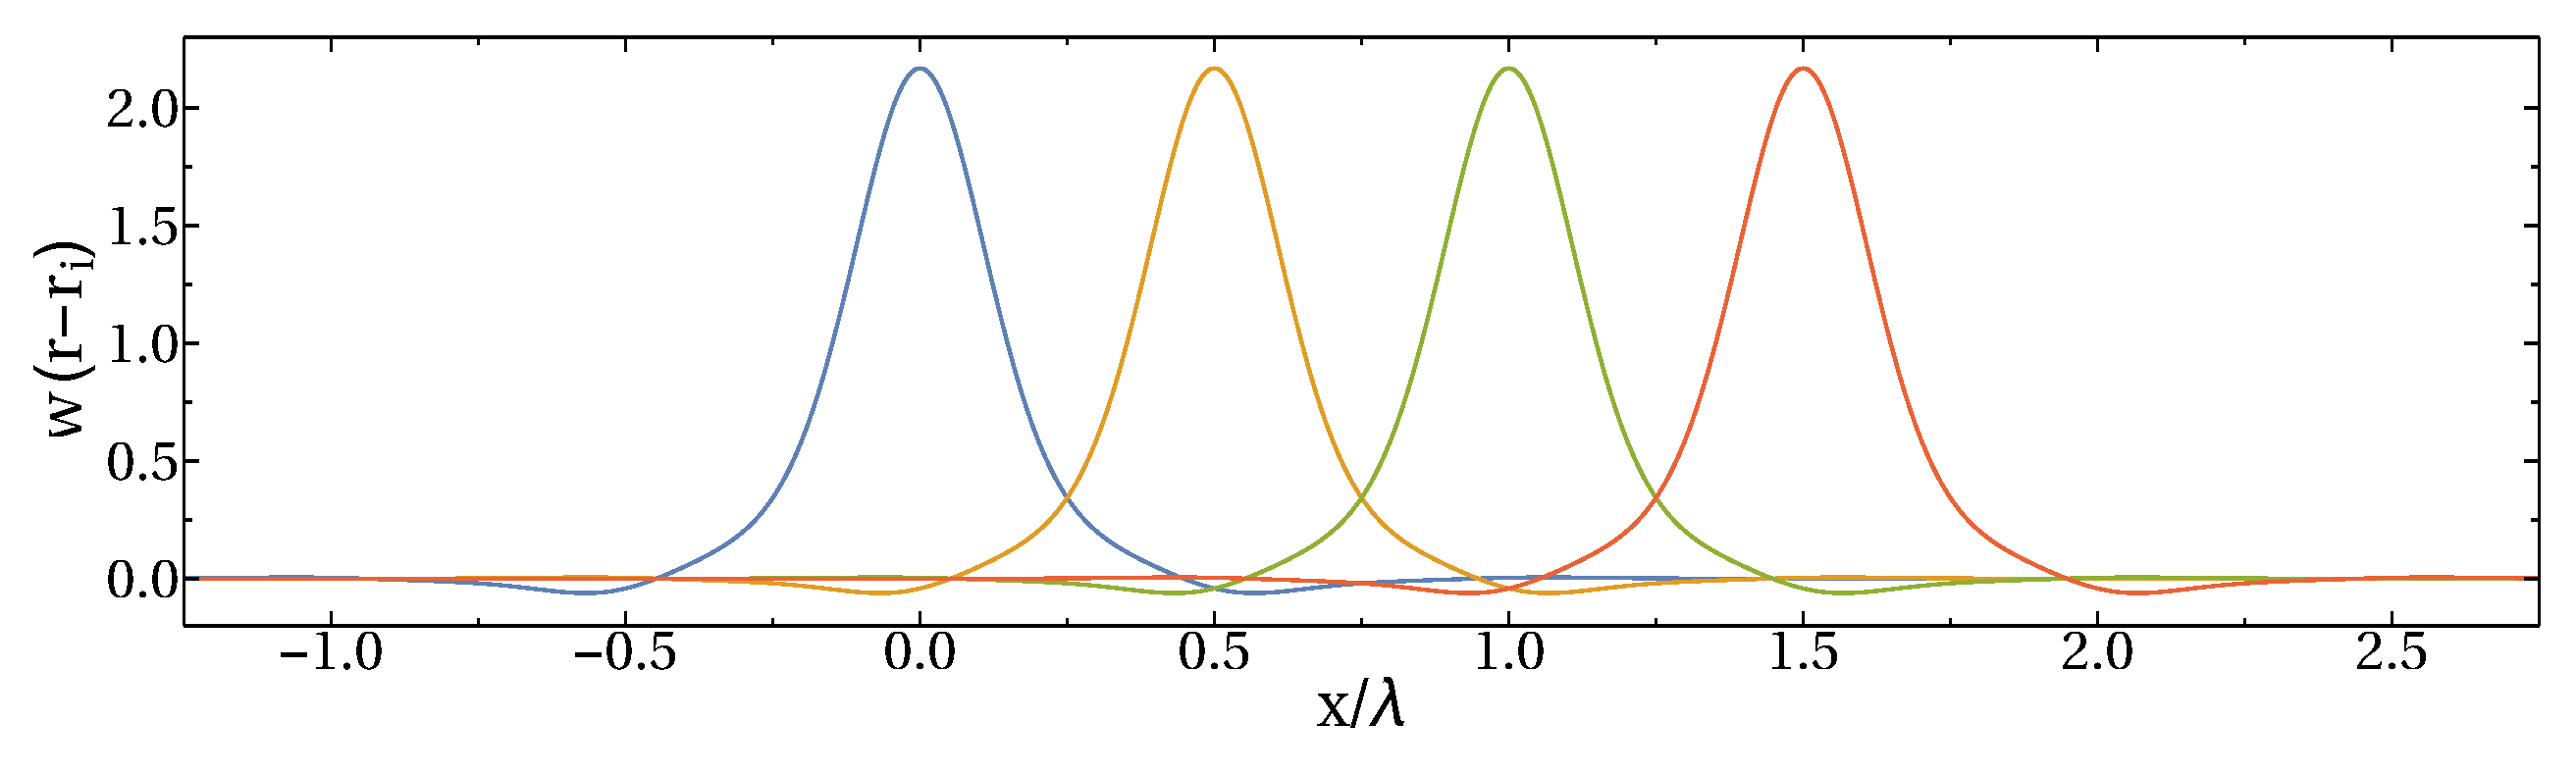
\includegraphics[width=1.0\textwidth]{Wannier1}
  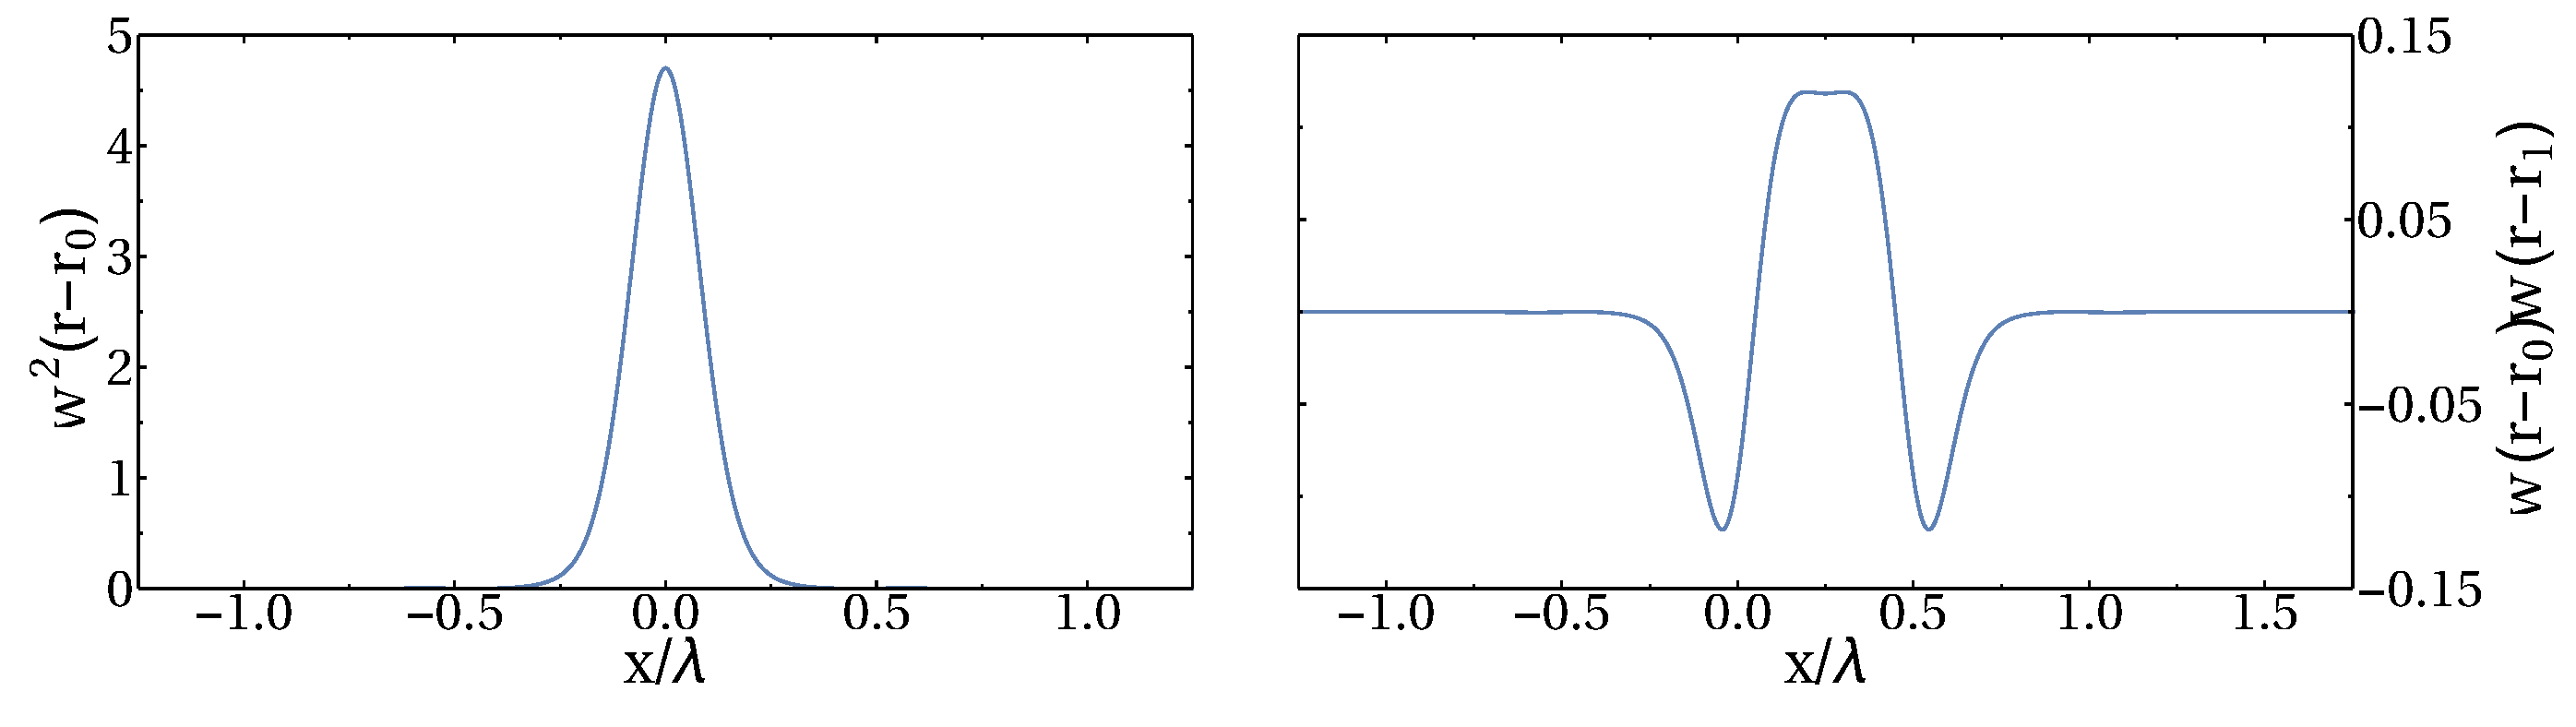
\includegraphics[width=1.0\textwidth]{Wannier2}
  \caption[Wannier Function Overlaps]{(a) The Wannier functions
    corresponding to four neighbouring sites in a 1D
    lattice. $\lambda$ is the wavelength of the trapping beams, thus
    lattice sites occur every $\lambda/2$. (Bottom Left) The square of
    a single Wannier function - this quantity is used when evaluating
    $\hat{D}$. It's much larger than the overlap between two
    neighbouring Wannier functions, but it is localised to the
    position of the lattice site it belongs to. (Bottom Right) The
    overlap of two neighbouring Wannier functions - this quantity is
    used when evaluating $\hat{B}$. It is much smaller than the square
    of a Wannier function, but since it's localised in between the
    sites, thus $\hat{B}$ can be maximised while $\hat{D}$ minimised
    by focusing the light in between the sites.}
  \label{fig:WannierOverlaps}
\end{figure}

\mynote{show the expansion into an FT}
In order to calculate the $J_{i,j}$ coefficients we perform numerical
calculations using realistic Wannier functions. However, it is
possible to gain some analytic insight into the behaviour of these
values by looking at the Fourier transforms of the Wannier function
overlaps, $\mathcal{F}[W_{0,1}](k)$, shown in Fig.
\ref{fig:WannierFT}b. This is because the light mode product,
$u_1^*(x) u_0(x)$, can be in general decomposed into a sum of
oscillating exponentials of the form $e^{i k x}$ making the integral
in Eq. \eqref{eq:Jcoeff} a sum of Fourier transforms of
$W_{0,1}(x)$. We consider both the detected and probe beam to be
standing waves which gives the following expressions for the $\hat{D}$
and $\hat{B}$ operators
\begin{eqnarray}
  \label{eq:FTs}
  \hat{D} =
  \frac{1}{2}[\mathcal{F}[W_0](k_-)\sum_m\hat{n}_m\cos(k_- x_m
    +\varphi_-)
    \nonumber\\ +\mathcal{F}[W_0](k_+)\sum_m\hat{n}_m\cos(k_+
    x_m +\varphi_+)], \nonumber\\ \hat{B} =
  \frac{1}{2}[\mathcal{F}[W_1](k_-)\sum_m\hat{B}_m\cos(k_- x_m
    +\frac{k_-d}{2}+\varphi_-)
    \nonumber\\ +\mathcal{F}[W_1](k_+)\sum_m\hat{B}_m\cos(k_+
    x_m +\frac{k_+d}{2}+\varphi_+)],
\end{eqnarray}
where $k_\pm = k_{0x} \pm k_{1x}$, $k_{(0,1)x} = k_{0,1}
\sin(\theta_{0,1}$), $\hat{B}_m=b^\dag_mb_{m+1}+b_mb^\dag_{m+1}$, and
$\varphi_\pm=\varphi_0 \pm \varphi_1$. The key result is that the
$\hat{B}$ operator is phase shifted by $k_\pm d/2$ with respect to the
$\hat{D}$ operator since it depends on the amplitude of light in
between the lattice sites and not at the positions of the atoms,
allowing to decouple them at specific angles.

\begin{figure}[htbp!]
  \begin{center}
    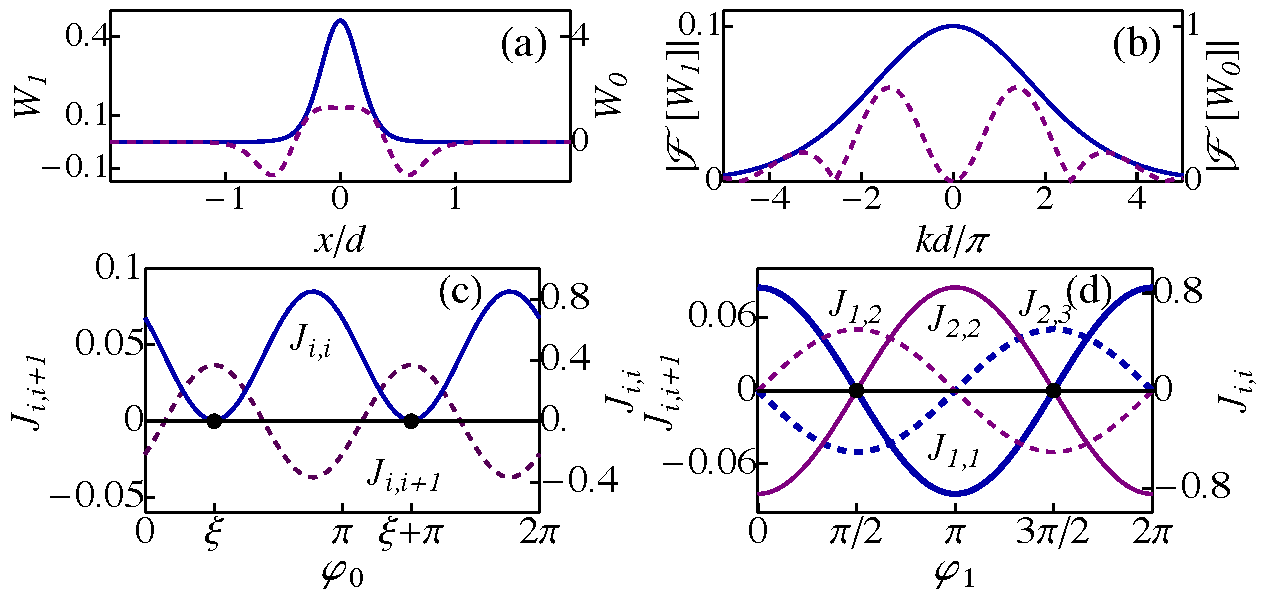
\includegraphics[width=\linewidth]{WF_S}
  \end{center}
  \caption[Wannier Function Fourier Transforms]{The Wannier function
    products: (a) $W_0(x)$ (solid line, right axis), $W_1(x)$ (dashed
    line, left axis) and their (b) Fourier transforms
    $\mathcal{F}[W_{0,1}]$. The Density $J_{i,i}$ and
    matter-interference $J_{i,i+1}$ coefficients in diffraction
    maximum (c) and minimum (d) as are shown as functions of standing
    wave shifts $\varphi$ or, if one were to measure the quadrature
    variance $(\Delta X^F_\beta)^2$, the local oscillator phase
    $\beta$. The black points indicate the positions, where light
    measures matter interference $\hat{B} \ne 0$, and the density-term
    is suppressed, $\hat{D} = 0$. The trapping potential depth is
    approximately 5 recoil energies.}
  \label{fig:WannierFT}
\end{figure}

The simplest case is to find a diffraction maximum where $J_{i,i+1} =
J_B$. This can be achieved by crossing the light modes such that
$\theta_0 = -\theta_1$ and $k_{0x} = k_{1x} = \pi/d$ and choosing the
light mode phases such that $\varphi_+ = 0$. Fig. \ref{fig:WannierFT}c
shows the value of the $J_{i,j}$ coefficients under these
circumstances. In order to make the $\hat{B}$ contribution to light
scattering dominant we need to set $\hat{D} = 0$ which from
Eq. \eqref{eq:FTs} we see is possible if $\varphi_0 = -\varphi_1 =
\arccos[-\mathcal{F}[W_0](2\pi/d)/\mathcal{F}[W_0](0)]/2$. This
arrangement of light modes maximizes the interference signal,
$\hat{B}$, by suppressing the density signal, $\hat{D}$, via
interference compensating for the spreading of the Wannier
functions. 

Another possibility is to obtain an alternating pattern similar
corresponding to a classical diffraction minimum. We consider an
arrangement where the beams are arranged such that $k_{0x} = 0$ and
$k_{1x} = \pi/d$ which gives the following expressions for the density
and interference terms
\begin{eqnarray}
  \label{eq:DMin}
	\hat{D} = \mathcal{F}[W_0](\pi/d) \sum_m (-1)^m \hat{n}_m
        \cos(\varphi_0) \cos(\varphi_1) \nonumber \\ \hat{B} =
        -\mathcal{F}[W_1](\pi/d) \sum_m (-1)^m \hat{B}_m
        \cos(\varphi_0) \sin(\varphi_1).
\end{eqnarray}
The corresponding $J_{i,j}$ coefficients are shown in
Fig. \ref{fig:WannierFT}d for $\varphi_0=0$. It is clear that for
$\varphi_1 = \pm \pi/2$, $\hat{D} = 0$, which is intuitive as this
places the lattice sites at the nodes of the mode $u_1(x)$. This is a
diffraction minimum as the light amplitude is also zero, $\langle
\hat{B} \rangle = 0$, because contributions from alternating
inter-site regions interfere destructively. However, the intensity
$\langle \ad_1 \a \rangle = |C|^2 \langle \hat{B}^2 \rangle$ is
proportional to the variance of $\hat{B}$ and is non-zero. 

\mynote{explain quadrature}
Alternatively, one can use the arrangement for a diffraction minimum
described above, but use travelling instead of standing waves for the
probe and detected beams and measure the light quadrature variance. In
this case $\hat{X}^F_\beta = \hat{D} \cos(\beta) + \hat{B}
\sin(\beta)$ and by varying the local oscillator phase, one can choose
which conjugate operator to measure.

\mynote{fix labels}
\begin{figure}[hbtp!]
	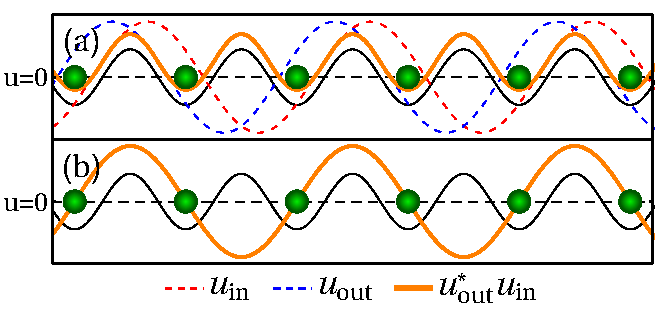
\includegraphics[width=\linewidth]{BDiagram}
	\caption[Maximising Light-Matter Coupling between Lattice
          Sites]{Light field arrangements which maximise coupling,
          $u_1^*u_0$, between lattice sites. The thin black line
          indicates the trapping potential (not to scale). (a)
          Arrangement for the uniform pattern $J_{m,m+1} = J_1$. (b)
          Arrangement for spatially varying pattern $J_{m,m+1}=(-1)^m
          J_2$; here $u_0=1$ so it is not shown and $u_1$ is real thus
          $u_1^*u_0=u_1$. \label{fig:BDiagram}}
\end{figure}

\subsection{Electric Field Stength}

The Electric field operator at position $\b{r}$ and at time $t$ is
usually written in terms of its positive and negative components:
\begin{equation}
  \b{\hat{E}}(\b{r},t) = \b{\hat{E}}^{(+)}(\b{r},t) + \b{\hat{E}}^{(-)}(\b{r},t),
\end{equation}
where
\begin{subequations}
  \begin{equation}
    \b{\hat{E}}^{(+)}(\b{r},t) = \sum_{\b{k}} \hat{\epsilon}_{\b{k}} 
    \mathcal{E}_{\b{k}} \a_{\b{k}} e^{-i \omega_{\b{k}} t + i \b{k} \cdot \b{r}},
  \end{equation}
  \begin{equation}
    \b{\hat{E}}^{(-)}(\b{r},t) = \sum_{\b{k}} \hat{\epsilon}_{\b{k}} 
    \mathcal{E}_{\b{k}} \a^\dagger_{\b{k}} e^{i \omega_{\b{k}} t - i \b{k} \cdot \b{r}},
  \end{equation}
\end{subequations}
$\hat{\epsilon}_{\b{k}}$ is a unit polarization vector, $\b{k}$ is the
wave vector,
$\mathcal{E}_{\b{k}} = \sqrt{\hbar \omega_{\b{k}} / 2 \epsilon_0 V}$,
$\epsilon_0$ is the free space permittivity, $V$ is the quantization
volume and $\a_\b{k}$ and $\a_\b{k}^\dagger$ are the annihilation and
creation operators respectively of a photon in mode $\b{k}$, and
$\omega_\b{k}$ is the angular frequency of mode $\b{k}$.

In Ref. \cite{Scully} it was shown that the operator
$\b{\hat{E}}^{(+)}(\b{r},t)$ due to light scattering from a single
atom located at $\b{r}^\prime$ at the observation point $\b{r}$ is
given by
\begin{equation}
  \label{eq:Ep}
  \b{\hat{E}}^{(+)}(\b{r},\b{r}^\prime,t) = \frac{\omega_a^2 d \sin \eta}{4 \pi
    \epsilon_0 c^2 |\b{r} - \b{r}^\prime|} \hat{\epsilon} \sigma^-
  \left( \b{r}^\prime, t - \frac{|\b{r} - \b{r}^\prime|}{c} \right),
\end{equation}
with a similar expression for
$\b{E}^{(-)}(\b{r},\b{r}^\prime,t)$. Eq. \eqref{eq:Ep} is valid only
in the far field, $\eta$ is the angle the dipole makes with
$\b{r} - \b{r}^\prime$, $\hat{\epsilon}$ is the polarization vector
which is perpendicular to $\b{r} - \b{r}^\prime$ and lies in the plane
defined by $\b{r} - \b{r}^\prime$ and the dipole, $\omega_a$ is the
atomic transition frequency, and $d$ is the dipole matrix element
between the two levels, and $c$ is the speed of light in vacuum.


We have already derived an expression for the atomic lowering
operator, $\sigma^-$, in Eq. \eqref{eq:sigmam} and it is given by
\begin{equation}
  \sigma^-(\b{r}, t) = - \frac{i} {\Delta_a} \sum_\b{k} g_\b{k}
  a_\b{k}(t) u_\b{k}(\b{r}).
\end{equation}
We will want to substitute this expression into Eq. \eqref{eq:Ep}, but
first we note that in the setup we consider the coherent probe will be
much stronger than the scattered modes. This in turn implies that the
expression for $\sigma^-$ will be dominated by this external
probe. Therefore, we drop the sum and consider only a single wave
vector, $\b{k}_0$, of the dominant contribution from the external
beam corresponding to the mode $\a_0$.

We now use the definititon of the atom-light coupling constant
\cite{Scully} to make the substitution
$g_0 a_0 = -i \Omega_0 e^{-i \omega_0 t} / 2$, where
$\Omega_0$ is the Rabi frequency for the probe-atom system. We now
evaluate the polarisation operator at the retarded time
\begin{equation}
  \sigma^- \left(\b{r}^\prime, t - \frac{|\b{r} - \b{r}^\prime|}{c} \right) =
  -\frac{\Omega_0}{2 \Delta_a} u_0 (\b{r}^\prime) \exp \left[-i \omega_0
    \left( t - \frac{|\b{r} - \b{r}^\prime|}{c} \right)\right].
\end{equation}
We are considering observation in the far field regime so
$|\b{r} - \b{r}^\prime| \approx r - \hat{\b{r}} \cdot
\b{r}^\prime$. We also consider the incoming, $\b{k}_0$, and the
outgoing, $\mathbf{k}_1$, waves to be of the same wavelength,
$|\b{k}_0| = |\b{k}_1| = k = \omega_0 / c$, hence
$(\omega_0 / c) |\b{r} - \b{r}^\prime| \approx k (r - \hat{\b{r}}
\cdot \b{r}^\prime) = \b{k}_1 \cdot (\b{r} - \b{r}^\prime )$ and
\begin{equation}
  \sigma^- \left(\b{r}^\prime, t - \frac{|\b{r} - \b{r}^\prime|}{c} \right) \approx
  -\frac{\Omega_0}{2 \Delta_a} u_0 (\b{r}^\prime) \exp \left[i
    \b{k}_1 \cdot (\b{r} - \b{r}^\prime ) - i \omega_0 t \right].
\end{equation}

The many-body version of the electric field operator is given by
\begin{equation}
  \b{\hat{E}}^{(+)}_N(\b{r},t) = \int \mathrm{d}^3 \b{r}^\prime
  \Psi^\dagger (\b{r}^\prime) \b{\hat{E}}^{(+)}(\b{r},\b{r}^\prime,t) \Psi(\b{r}^\prime),
\end{equation}
where $\Psi(\b{r})$ is the atomic matter-field operator. As before, we
expand this field operator using localized Wannier functions
corresponding to the lattice potential and keeping only the lowest
vibrational state at each site:
$\Psi(\b{r}) = \sum_i b_i w(\b{r} - \b{r}_i)$, where $b_i$ is the
annihilation operator of an atom at site $i$ with the coordinate
$\b{r}_i$. Thus, the relevant many-body operator is
\begin{subequations}
  \begin{equation}
    \b{\hat{E}}^{(+)}_N(\b{r},t) = \hat{\epsilon} C_E
    \sum_{i,j}^K \bd_i b_j \int \mathrm{d}^3 \b{r}^\prime
    w^* (\b{r}^\prime - \b{r}_i)  \frac{u_0
      (\b{r}^\prime)}{|\b{r} - \b{r}^\prime|} e^ {i \b{k}_1
      \cdot (\b{r} - \b{r}^\prime ) - i \omega_0 t }
    w(\b{r}^\prime - \b{r}_j),
  \end{equation}
  \begin{equation}
    C_E = -\frac{\omega_a^2 \Omega_0 d \sin \eta}{8 \pi \epsilon_0 c^2
      \Delta_a}
  \end{equation}
\end{subequations}
where $K$ is the number of illuminated sites. We now assume that the
lattice is deep and that the light scattering occurs on time scales
much shorter than atom tunneling. Therefore, we ignore all terms for
which $i \ne j$ and the remaining integrals become $\int \mathrm{d}^3
\b{r}_0 w^*(\b{r}_0 - \b{r}_i) f (\b{r})
w(\b{r}_0 - \b{r}_i) = f(\b{r}_i)$. The final form of
the many body operator is then
\begin{equation}
  \b{E}^{(+)}_N(\b{r},t) = \hat{\epsilon} C_E
  \sum_{j = 1}^K \hat{n}_j \frac{u_0 (\b{r}_j)}{|\b{r} -
    \b{r}_j|} e^ {i \b{k}_1 \cdot (\b{r} - \b{r}_j
    ) - i \omega_0 t },
\end{equation}
where $\hat{n}_i = b^\dagger_ib_i$ is the atom number operator at site
$i$. We will now consider the incoming probe to be a plane wave,
$u_0(\b{r}) = e^{i \b{k}_0 \cdot \b{r}}$, and we
approximate $|\b{r} - \b{r}_j| \approx r$ in the
denominator. Thus,
\begin{equation}
  \b{E}^{(+)}_N(\b{r},t) = \hat{\epsilon} C_E \frac{e^ {ikr - i\omega_0t}}{r}
  \sum_{j = 1}^K \hat{n}_j e^ {i (\b{k}_0 - \b{k}_1) \cdot \b{r}_j}.
\end{equation}
We note that this is exactly the same form of the optical field as
derived from a generalised Bose-Hubbard model which considers a fully
quantum light-matter interaction Hamiltonian \cite{mekhov2007prl,
  mekhov2007pra, mekhov2012}. We can even express the result in terms of
the $\hat{D} = \sum_j^K u_1^*(\b{r}_j) u_0(\b{r}_j)
\hat{n}_j$ formalism used in those works
\begin{equation}
  \b{E}^{(+)}_N(\b{r},t) = \hat{\epsilon} C_E \frac{e^
    {ikr - i\omega_0t}}{r} \hat{D}.
\end{equation}

The average light intensity at point $\b{r}$ at time $t$ is given
by the formula $I = c \epsilon_0 |E|^2/2$ and yields
\begin{equation}
  \langle I (\b{r}, t) \rangle = c \epsilon_0 \langle
  E^{(-)} (\b{r}, t) E^{(+)} (\b{r}, t) \rangle =
  \frac{c \epsilon_0}{r^2} C_E^2 \langle \hat{D}^* \hat{D} \rangle.
\end{equation}
The scattering is dominated by a uniform background for which $\langle
\hat{D}^* \hat{D} \rangle \approx N_K$ for a superfluid
\cite{mekhov2012}, where $N_K$ is the mean number of atoms in the
illuminated volume. Thus, the approximate number of photons scattered
per second can be obtained by integrating over a sphere
\begin{equation}
  n_{\Phi} = \frac{4 \pi c \epsilon_0}{3 \hbar \omega_a} \left(\frac{\omega_a^2
      \Omega_0 d}{8 \pi \epsilon_0 c^2 \Delta_a}\right)^2 N_K.
\end{equation}
In the Weisskopf-Wigner approximation it can be shown \cite{Scully}
that for a two level system the decay constant, $\Gamma$, is
\begin{equation}
  \Gamma = \frac{\omega_a^3 d^2}{3 \pi \epsilon_0 \hbar c^3}.
\end{equation}
Therefore, we can now express the quantity $n_{\Phi}$ as
\begin{equation}
  n_{\Phi} = \frac{1}{8} \left(\frac{\Omega_0}{\Delta_a}\right)^2 \frac{\Gamma}{2} N_K.
\end{equation}
Estimates of the scattering rate using real experimental parameters
are given in Table \ref{tab:photons}.

\begin{table}[!htbp]
  \centering
  \begin{tabular}{|c|c|c|}
    \hline
    Value & Miyake \emph{et al.} & Weitenberg \emph{et al.} \\ \hline
    $\omega_a$ & \multicolumn{2}{|c|}{$2 \pi \cdot 384$ THz}\\ \hline
    $\Gamma$ & \multicolumn{2}{|c|}{$2 \pi \cdot 6.07$ MHz} \\ \hline
    $\Delta_a$ & $2\pi \cdot 30$ MHz & $2 \pi \cdot 85$ MHz \\ \hline
    $I$ & $4250$ Wm$^{-2}$ & N/A \\ \hline
    $\Omega_0$ & 293$\times 10^6$ s$^{-1}$ & 42.5$\times 10^6$ s$^{-1}$ \\ \hline
    $N_K$ & 10$^5$ & 147 \\ \hline \hline
    $n_{\Phi}$ & $6 \times 10^{11}$ s$^{-1}$ & $2 \times 10^6$ s$^{-1}$ \\ \hline
  \end{tabular}
  \caption[Photon Scattering Rates]{ Rubidium data taken from
    Ref. \cite{steck}; Miyake \emph{et al.}: based on
    Ref. \cite{miyake2011}. The $5^2S_{1/2}$, $F=2 \rightarrow
    5^2P_{3/2}$, $F^\prime = 3$ transition of $^{87}$Rb is
    considered. For this transition the Rabi frequency is actually
    larger than the detuning and and effects of saturation should be
    taken into account in a more complete analysis. However, it is
    included for discussion. The detuning is said to be a few natural
    linewidths. Note that it is much smaller than $\Omega_0$. The Rabi
    fequency is $\Omega_0 = (d_\mathrm{eff}/\hbar)\sqrt{2 I / c
      \epsilon_0}$ which is obtained from definition of Rabi
    frequency, $\Omega = \mathbf{d} \cdot \mathbf{E} / \hbar$,
    assuming the electric field is parallel to the dipole, and the
    relation $I = c \epsilon_0 |E|^2 /2$. We used $d_\mathrm{eff} =
    1.73 \times 10^{-29}$ Cm \cite{steck}; Weitenberg \emph{et al.}:
    based on Ref. \cite{weitenberg2011, weitenbergThesis}. The
    $5^2S_{1/2} \rightarrow 5^2P_{3/2}$ transition of $^{87}$Rb is
    used. Ref. \cite{weitenberg2011} gives the free space detuning to
    be $\Delta_\mathrm{free} = - 2 \pi \cdot 45$
    MHz. Ref. \cite{weitenbergThesis} clarifies that the relevant
    detuning is $\Delta = \Delta_\mathrm{free} + \Delta_\mathrm{lat}$,
    where $\Delta_\mathrm{lat} = - 2 \pi \cdot 40$
    MHz. Ref. \cite{weitenbergThesis} uses a saturation parameter
    $s_\mathrm{tot}$ to quantify the intensity of the beams which is
    related to the Rabi frequency, $s_\mathrm{tot} = 2 \Omega^2 /
    \Gamma^2$ \cite{steck,foot}. We can extract $s_\mathrm{tot}$ for
    the experiment from the total scattering rate by
    $\Gamma_\mathrm{sc} = (\Gamma/2) (s_\mathrm{tot}) /
    (1+s_\mathrm{tot}+(2 \Delta / \Gamma)^2)$. A scattering rate of 60
    kHz per atom \cite{weitenberg2011} gives $s_\mathrm{tot} = 2.5$.}
  \label{tab:photons}
\end{table}

%*******************************************************************************
%*********************************** Third Chapter *****************************
%*******************************************************************************

\chapter{Probing Correlations by Global 
Nondestructive Addressing} %Title of the Third Chapter

\ifpdf
    \graphicspath{{Chapter3/Figs/Raster/}{Chapter3/Figs/PDF/}{Chapter3/Figs/}}
\else
    \graphicspath{{Chapter3/Figs/Vector/}{Chapter3/Figs/}}
\fi


%********************************** %First Section  **************************************

\section{Introduction}

Having developed the basic theoretical framework within which we can
treat the fully quantum regime of light-matter interactions we now
consider possible applications. There are three prominent directions
in which we can proceed: nondestructive probing of the quantum state
of matter, quantum measurement backaction induced dynamics and quantum
optical lattices. Here, we deal with the first of the three options.

In this chapter we develop a method to measure properties of ultracold
gases in optical lattices by light scattering. In the previous chapter
we have shown that quantum light field couples to the bosons via the
operator $\hat{F}$. This is the key element of the scheme we propose
as this makes it sensitive to the quantum state of the matter and all
of its possible superpositions which will be reflected in the quantum
state of the light itself. We have also shown in section
\ref{sec:derivation} that this coupling consists of two parts, a
density component $\hat{D}$ given by Eq. \eqref{eq:D}, and a phase
component $\hat{B}$ given by Eq. \eqref{eq:B}. Therefore, when probing
the quantum state of the ultracold gas we can have access to not only
density correlations, but also matter-field interference at its
shortest possible distance in an optical lattice, i.e.~the lattice
period. Previous work on quantum non-demolition (QND) schemes
\cite{rogers2014, mekhov2007prl, eckert2008} probe only the density
component as it is generally challenging to couple to the matter-field
observables directly. Here, we will consider nondestructive probing of
both density and interference operators.

Firstly, we will consider the simpler and more typical case of
coupling to the atom number operators via $\hat{F} =
\hat{D}$. However, we show that light diffraction in this regime has
several nontrivial characteristics due to the fully quantum nature of
the interaction. Firstly, we show that the angular distribution has
multiple interesting features even when classical diffraction is
forbidden facilitating their experimental observation. We derive new
generalised Bragg diffraction conditions which are different to their
classical counterpart. Furthermore, due to the fully quantum nature of
the interaction our proposal is capable of probing the quantum state
beyond mean-field prediction. We demonstrate this by showing that this
scheme is capable of distinguishing all three phases in the Mott
insulator - superfluid - Bose glass phase transition in a 1D
disordered optical lattice which is not very well described by a
mean-field treatment. We underline that transitions in 1D are much
more visible when changing an atomic density rather than for
fixed-density scattering. It was only recently that an experiment
distinguished a Mott insulator from a Bose glass \cite{derrico2014}
via a series of destructive measurements. Our proposal, on the other
hand, is nondestructive and is capable of extracting all the relevant
information in a single experiment.

Having shown the possibilities created by this nondestructive
measurement scheme we move on to considering light scattering from the
phase related observables via the operator $\hat{F} = \hat{B}$. This
enables in-situ probing of the matter-field coherence at its shortest
possible distance in an optical lattice, i.e. the lattice period,
which defines key processes such as tunnelling, currents, phase
gradients, etc. This is in contrast to standard destructive
time-of-flight measurements which deal with far-field interference
although a relatively near-field scheme was use in
Ref. \cite{miyake2011}. We show how within the mean-field treatment,
this enables measurements of the order parameter, matter-field
quadratures and squeezing. This can have an impact on atom-wave
metrology and information processing in areas where quantum optics
already made progress, e.g., quantum imaging with pixellized sources
of non-classical light \cite{golubev2010, kolobov1999}, as an optical
lattice is a natural source of multimode nonclassical matter waves.

\section{Coupling to the Quantum State of Matter}

As we have seen in section \ref{sec:a} under certain approximations
the scattered light mode, $\a_1$, is linked to the quantum state of
matter via 
\begin{equation}
  \label{eq:a-3}
  \a_1 = C \hat{F} = C \left(\hat{D} + \hat{B} \right),
\end{equation}
where the atomic operators $\hat{D}$ and $\hat{B}$, given by
Eq. \eqref{eq:D} and Eq. \eqref{eq:B}, are responsible for the
coupling to on-site density and inter-site interference
respectively. It is crucial to note that light couples to the bosons
via an operator as this makes it sensitive to the quantum state of the
matter as this will imprint the fluctuations in the quantum state of
the scattered light.

Here, we will use this fact that the light is sensitive to the atomic
quantum state due to the coupling of the optical and matter fields via
operators in order to develop a method to probe the properties of an
ultracold gas. Therefore, we neglect the measurement back-action and
we will only consider expectation values of light observables. Since
the scheme is nondestructive (in some cases, it even satisfies the
stricter requirements for a QND measurement \cite{mekhov2012,
  mekhov2007pra}) and the measurement only weakly perturbs the system,
many consecutive measurements can be carried out with the same atoms
without preparing a new sample. We will show how the extreme
flexibility of the the measurement operator $\hat{F}$ allows us to
probe a variety of different atomic properties in-situ ranging from
density correlations to matter-field interference.

\subsection{On-site Density Measurements}

We have seen in section \ref{sec:B} that typically the dominant term
in $\hat{F}$ is the density term $\hat{D}$ \cite{LP2009,
  mekhov2007pra, rist2010, lakomy2009, ruostekoski2009}. This is
simply due to the fact that atoms are localised with lattice sites
leading to an effective coupling with atom number operators instead of
inter-site interference terms. Therefore, we will first consider
nondestructive probing of the density related observables of the
quantum gas. However, we will focus on the novel nontrivial aspects
that go beyond the work in Ref. \cite{mekhov2012, mekhov2007prl,
  mekhov2007pra} which only considered a few extremal cases.

As we are only interested in the quantum information imprinted in the
state of the optical field we will simplify our analysis by
considering the light scattering to be much faster than the atomic
tunnelling. Therefore, our scheme is actually a QND scheme
\cite{rogers2014, mekhov2007prl, mekhov2007pra, eckert2008} as
normally density-related measurements destroy the matter-phase
coherence since it is its conjugate variable, but here we neglect the
$\bd_i b_j$ terms. Furthermore, we will consider a deep
lattice. Therefore, the Wannier functions will be well localised
within their corresponding lattice sites and thus the coefficients
$J_{i,i}$ reduce to $u_1^*(\b{r}_i) u_0(\b{r}_i)$ leading to
\begin{equation}
  \label{eq:D-3}
  \hat{D}=\sum_i^K u_1^*(\b{r}_i) u_0(\b{r}_i) \hat{n}_i,
\end{equation} 
which for travelling
[$u_l(\b{r})=\exp(i \b{k}_l \cdot \b{r}+i\varphi_l)$] or standing
[$u_l(\b{r})=\cos(\b{k}_l \cdot \b{r}+\varphi_l)$] waves is just a
density Fourier transform at one or several wave vectors
$\pm(\b{k}_1 \pm \b{k}_0)$. 

We will now define a new auxiliary quantity to aid our analysis,
\begin{equation}
  \label{eq:R}
  R = \langle \ad_1 \a_1 \rangle - | \langle \a_1 \rangle |^2,
\end{equation}
which we will call the ``quantum addition'' to light scattering. By
construction $R$ is simply the full light intensity minus the
classical field diffraction. In order to justify its name we will show
that this quantity depends purely quantum mechanical properties of the
ultracold gase. We will substitute $\a_1 = C \hat{D}$ using
Eq. \eqref{eq:D-3} into our expression for $R$ in Eq. \eqref{eq:R} and
we will make use of the shorthand notation
$A_i = u_1^*(\b{r}_i) u_0(\b{r}_i)$. The result is
\begin{equation}
  R = |C|^2 \sum_{i,j}^K A^*_i A_j \langle \delta \hat{n}_i \delta
  \hat{n}_j \rangle,
\end{equation}
where $\delta \hat{n}_i = \hat{n}_i - \langle \hat{n}_i
\rangle$. Thus, we can clearly see that $R$ is a result of light
scattering from fluctuations in the atom number which is a purely
quantum mechanical property of a system. Therefore, $R$, the ``quantum
addition'' faithfully represents the new contribution from the quantum
light-matter interaction to the diffraction pattern.

If instead we are interested in quantities linear in $\hat{D}$, we can
measure the quadrature of the light fields which in section
\ref{sec:a} we saw that $\hat{X}_\phi = |C| \hat{X}^F_\beta$. For the
case when both the scattered mode and probe are travelling waves the
quadrature
\begin{equation} 
  \hat{X}^F_\beta = \frac{1}{2} \left( \hat{F} e^{-i \beta} +
    \hat{F}^\dagger e^{i \beta} \right) = \sum_i^K \hat{n}_i\cos[(\b{k}_1 - \b{k}_2) \cdot
  \b{r}_i - \beta].
\end{equation} 
Note that different light quadratures are differently coupled to the
atom distribution, hence by varying the local oscillator phase, and
thus effectively $\beta$, and/or the detection angle one can scan the
whole range of couplings. A similar expression exists for $\hat{D}$
for a standing wave probe, where $\beta$ is replaced by $\varphi_0$,
and scanning is achieved by varying the position of the wave with
respect to atoms.

The ``quantum addition'', $R$, and the quadrature variance,
$(\Delta X^F_\beta)^2$, are both quadratic in $\a_1$. Therefore, they
will havea nontrivial angular dependence, showing more peaks than
classical diffraction. Furthermore, these peaks can be tuned very
easily with $\beta$ or $\varphi_l$. Fig. \ref{fig:scattering} shows
the angular dependence of $R$ for the case when the scattered mode is
a standing wave and the probe is a travelling wave scattering from
bosons in a 3D optical lattice. The first noticeable feature is the
isotropic background which does not exist in classical
diffraction. This background yields information about density
fluctuations which, according to mean-field estimates (i.e.~inter-site
correlations are ignored), are related by
$R = K( \langle \hat{n}^2 \rangle - \langle \hat{n} \rangle^2 )/2$. In
Fig. \ref{fig:scattering} we can see a significant signal of
$R = |C|^2 N_K/2$, because it shows scattering from an ideal
superfluid which has significant density fluctuations with
correlations of infinte range. However, as the parameters of the
lattice are tuned across the phase transition into a Mott insulator
the signal goes to zero. This is because the Mott insulating phase has
well localised atoms at each site which suppresses density
fluctuations entirely leading to absolutely no ``quantum addition''.

\begin{figure}[htbp!]
  \centering
  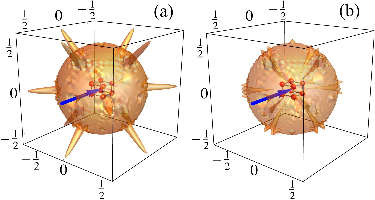
\includegraphics[width=\linewidth]{Ep1}
  \caption[Light Scattering Angular Distribution]{Light intensity
    scattered into a standing wave mode from a superfluid in a 3D
    lattice (units of $R/(|C|^2N_K)$). Arrows denote incoming
    travelling wave probes. The classical Bragg condition,
    $\Delta \b{k} = \b{G}$, is not fulfilled, so there is no classical
    diffraction, but intensity still shows multiple peaks, whose
    heights are tunable by simple phase shifts of the optical beams:
    (a) $\varphi_1=0$; (b) $\varphi_1=\pi/2$. Interestingly, there is
    also a significant uniform background level of scattering which
    does not occur in its classical counterpart. }
  \label{fig:scattering}
\end{figure}

We can also observe maxima at several different angles in
Fig. \ref{fig:scattering}. Interestingly, they occur at different
angles than predicted by the classical Bragg condition. Moreover, the
classical Bragg condition is actually not satisfied which means there
actually is no classical diffraction on top of the ``quantum
addition'' shown here. Therefore, these features would be easy to see
in an experiment as they wouldn't be masked by a stronger classical
signal.  We can even derive the generalised Bragg conditions for the
peaks that we can see in Fig. \ref{fig:scattering}. 

% Derive and show these Bragg conditions

As $(\Delta X^F_\beta)^2$ and $R$ are quadratic variables,
the generalized Bragg conditions for the peaks are
$2 \Delta \b{k} = \b{G}$ for quadratures of travelling waves, where
$\Delta \b{k} = \b{k}_0 - \b{k}_1$ and $\b{G}$ is the reciprocal
lattice vector, and $2 \b{k}_1 = \b{G}$ for standing wave $\a_1$ and
travelling $\a_0$, which is clearly different from the classical Bragg
condition $\Delta \b{k} = \b{G}$. The peak height is tunable by the
local oscillator phase or standing wave shift as seen in Fig.
\ref{fig:scattering}b.

In section \ref{sec:Efield} we have estimated the mean photon
scattering rates integrated over the solid angle for the only two
experiments so far on light diffraction from truly ultracold bosons
where the measurement object was light
\begin{equation} 
  n_{\Phi}= \left(\frac{\Omega_0}{\Delta_a}\right)^2 \frac{\Gamma K}{8}
  (\langle\hat{n}^2\rangle-\langle\hat{n}\rangle^2).
\end{equation} 
Therefore, applying these results to the scattering patters in
Fig. \ref{fig:scattering} the background signal should reach
$n_\Phi \approx 10^6$ s$^{-1}$ in Ref. \cite{weitenberg2011} (150
atoms in 2D), and $n_\Phi \approx 10^{11}$ s$^{-1}$ in
Ref. \cite{miyake2011} ($10^5$ atoms in 3D). These numbers show that
the diffraction patterns we have seen due to the ``quantum addition''
should be visible using currently available technology, especially
since the most prominent features, such as Bragg diffraction peaks, do
not coincide at all with the classical diffraction pattern.

\subsection{Mapping the quantum phase diagram}

\begin{figure}[htbp!]  
  \centering
  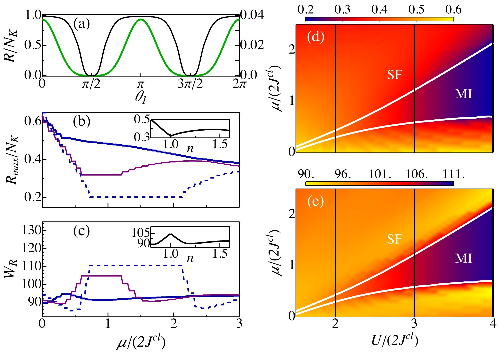
\includegraphics[width=\linewidth]{oph11}
  \caption[Mapping the Bose-Hubbard Phase Diagram]{(a) The angular
    dependence of scattered light $R$ for a superfluid (thin black,
    left scale, $U/2J^\text{cl} = 0$) and Mott insulator (thick green,
    right scale, $U/2J^\text{cl} =10$). The two phases differ in both
    their value of $R_\text{max}$ as well as $W_R$ showing that
    density correlations in the two phases differ in magnitude as well
    as extent. Light scattering maximum $R_\text{max}$ is shown in (b,
    d) and the width $W_R$ in (c, e).  It is very clear that varying
    chemical potential $\mu$ or density $\langle n\rangle$ sharply
    identifies the superfluid-Mott insulator transition in both
    quantities. (b) and (c) are cross-sections of the phase diagrams
    (d) and (e) at $U/2J^\text{cl}=2$ (thick blue), 3 (thin purple),
    and 4 (dashed blue). Insets show density dependencies for the
    $U/(2 J^\text{cl}) = 3$ line. $K=M=N=25$.}
	\label{fig:SFMI}
\end{figure}

We have shown how in mean-field, we can track the order parameter,
$\Phi$, by probing the matter-field interference using the coupling of
light to the $\hat{B}$ operator. In this case, it is very easy to
follow the superfluid to Mott insulator quantum phase transition since
we have direct access to the order parameter which goes to zero in the
insulating phase. In fact, if we're only interested in the critical
point, we only need access to any quantity that yields information
about density fluctuations which also go to zero in the MI phase and
this can be obtained by measuring
$\langle \hat{D}^\dagger \hat{D} \rangle$. However, there are many
situations where the mean-field approximation is not a valid
description of the physics. A prominent example is the Bose-Hubbard
model in 1D \cite{cazalilla2011, ejima2011, kuhner2000, pino2012,
  pino2013}. Observing the transition in 1D by light at fixed density
was considered to be difficult \cite{rogers2014} or even impossible
\cite{roth2003}. By contrast, here we propose varying the density or
chemical potential, which sharply identifies the transition. We
perform these calculations numerically by calculating the ground state
using DMRG methods \cite{tnt} from which we can compute all the
necessary atomic observables. Experiments typically use an additional
harmonic confining potential on top of the optical lattice to keep the
atoms in place which means that the chemical potential will vary in
space. However, with careful consideration of the full
($\mu/2J^\text{cl}$, $U/2J^\text{cl}$) phase diagrams in
Fig. \ref{fig:SFMI}(d,e) our analysis can still be applied to the
system \cite{batrouni2002}.

The 1D phase transition is best understood in terms of two-point
correlations as a function of their separation \cite{giamarchi}. In
the Mott insulating phase, the two-point correlations
$\langle \bd_i b_j \rangle$ and
$\langle \delta \hat{n}_i \delta \hat{n}_j \rangle$
($\delta \hat{n}_i =\hat{n}_i-\langle \hat{n}_i\rangle$) decay
exponentially with $|i-j|$. On the other hand the superfluid will
exhibit long-range order which in dimensions higher than one,
manifests itself with an infinite correlation length. However, in 1D
only pseudo long-range order happens and both the matter-field and
density fluctuation correlations decay algebraically \cite{giamarchi}.

The method we propose gives us direct access to the structure factor,
which is a function of the two-point correlation $\langle \delta
\hat{n}_i \delta \hat{n}_j \rangle$, by measuring the light
intensity. For two travelling waves maximally coupled to the density
(atoms are at light intensity maxima so $\hat{F} = \hat{D}$), the
quantum addition is given by
\begin{equation} 
  R =\sum_{i, j} \exp[i (\mathbf{k}_1 - \mathbf{k}_0)
  (\mathbf{r}_i - \mathbf{r}_j)] \langle \delta \hat{n}_i \delta
  \hat{n}_j \rangle,
\end{equation}

The angular dependence of $R$ for a Mott insulator and a superfluid is
shown in Fig. \ref{fig:SFMI}a, and there are two variables
distinguishing the states. Firstly, maximal $R$,
$R_\text{max} \propto \sum_i \langle \delta \hat{n}_i^2 \rangle$,
probes the fluctuations and compressibility $\kappa'$
($\langle \delta \hat{n}^2_i \rangle \propto \kappa' \langle \hat{n}_i
\rangle$).  The Mott insulator is incompressible and thus will have
very small on-site fluctuations and it will scatter little light
leading to a small $R_\text{max}$. The deeper the system is in the MI
phase (i.e. that larger the $U/2J^\text{cl}$ ratio is), the smaller
these values will be until ultimately it will scatter no light at all
in the $U \rightarrow \infty$ limit. In Fig. \ref{fig:SFMI}a this can
be seen in the value of the peak in $R$. The value $R_\text{max}$ in
the SF phase ($U/2J^\text{cl} = 0$) is larger than its value in the MI
phase ($U/2J^\text{cl} = 10$) by a factor of
$\sim$25. Figs. \ref{fig:SFMI}(b,d) show how the value of
$R_\text{max}$ changes across the phase transition. We see that the
transition shows up very sharply as $\mu$ is varied.

Secondly, being a Fourier transform, the width $W_R$ of the dip in $R$
is a direct measure of the correlation length $l$, $W_R \propto
1/l$. The Mott insulator being an insulating phase is characterised by
exponentially decaying correlations and as such it will have a very
large $W_R$. However, the superfluid in 1D exhibits pseudo long-range
order which manifests itself in algebraically decaying two-point
correlations \cite{giamarchi} which significantly reduces the dip in
the $R$. This can be seen in Fig. \ref{fig:SFMI}a and we can also see
that this identifies the phase transition very sharply as $\mu$ is
varied in Figs. \ref{fig:SFMI}(c,e). One possible concern with
experimentally measuring $W_R$ is that it might be obstructed by the
classical diffraction maxima which appear at angles corresponding to
the minima in $R$. However, the width of such a peak is much smaller
as its width is proportional to $1/M$.

It is also possible to analyse the phase transition quantitatively
using our method. Unlike in higher dimensions where an order parameter
can be easily defined within the MF approximation there is no such
quantity in 1D. However, a valid description of the relevant 1D low
energy physics is provided by Luttinger liquid theory
\cite{giamarchi}. In this model correlations in the supefluid phase as
well as the superfluid density itself are characterised by the
Tomonaga-Luttinger parameter, $K_b$. This parameter also identifies
the phase transition in the thermodynamic limit at $K_b = 1/2$. This
quantity can be extracted from various correlation functions and in
our case it can be extracted directly from $R$ \cite{ejima2011}. By
extracting this parameter from $R$ for various lattice lengths from
numerical DMRG calculations it was even possible to give a theoretical
estimate of the critical point for commensurate filling, $N = M$, in
the thermodynamic limit to occur at $U/2J^\text{cl} \approx 1.64$
\cite{ejima2011}. Our proposal provides a method to directly measure
$R$ in a lab which can then be used to experimentally determine the
location of the critical point in 1D.

So far both variables we considered, $R_\text{max}$ and $W_R$, provide
similar information. Next, we present a case where it is very
different. The Bose glass is a localized insulating phase with
exponentially decaying correlations but large compressibility and
on-site fluctuations in a disordered optical lattice. Therefore,
measuring both $R_\text{max}$ and $W_R$ will distinguish all the
phases. In a Bose glass we have finite compressibility, but
exponentially decaying correlations. This gives a large $R_\text{max}$
and a large $W_R$. A Mott insulator will also have exponentially
decaying correlations since it is an insulator, but it will be
incompressible. Thus, it will scatter light with a small
$R_\text{max}$ and large $W_R$. Finally, a superfluid will have long
range correlations and large compressibility which results in a large
$R_\text{max}$ and a small $W_R$.

\begin{figure}[htbp!]  
  \centering
  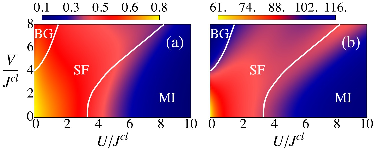
\includegraphics[width=\linewidth]{oph22}
  \caption[Mapping the Disoredered Phase Diagram]{The
    Mott-superfluid-glass phase diagrams for light scattering maximum
    $R_\text{max}/N_K$ (a) and width $W_R$ (b). Measurement of both
    quantities distinguish all three phases. Transition lines are
    shifted due to finite size effects \cite{roux2008}, but it is
    possible to apply well known numerical methods to extract these
    transition lines from such experimental data extracted from $R$
    \cite{ejima2011}. $K=M=N=35$.}
  \label{fig:BG}
\end{figure}

We confirm this in Fig. \ref{fig:BG} for simulations with the ratio of
superlattice- to trapping lattice-period $r\approx 0.77$ for various
disorder strengths $V$ \cite{roux2008}. Here, we only consider
calculations for a fixed density, because the usual interpretation of
the phase diagram in the ($\mu/2J^\text{cl}$, $U/2J^\text{cl}$) plane
for a fixed ratio $V/U$ becomes complicated due to the presence of
multiple compressible and incompressible phases between successive MI
lobes \cite{roux2008}. This way, we have limited our parameter space
to the three phases we are interested in: superfluid, Mott insulator,
and Bose glass. From Fig. \ref{fig:BG} we see that all three phases
can indeed be distinguished. In the 1D BHM there is no sharp MI-SF
phase transition in 1D at a fixed density \cite{cazalilla2011,
  ejima2011, kuhner2000, pino2012, pino2013} just like in
Figs. \ref{fig:SFMI}(d,e) if we follow the transition through the tip
of the lobe which corresponds to a line of unit density. However,
despite the lack of an easily distinguishable critical point it is
possible to quantitatively extract the location of the transition
lines by extracting the Tomonaga-Luttinger parameter from the
scattered light, $R$, in the same way it was done for an unperturbed
BHM \cite{ejima2011}.

Only recently \cite{derrico2014} a Bose glass phase was studied by
combined measurements of coherence, transport, and excitation spectra,
all of which are destructive techniques. Our method is simpler as it
only requires measurement of the quantity $R$ and additionally, it is
nondestructive.

\subsection{Matter-field interference measurements}

We now focus on enhancing the interference term $\hat{B}$ in the
operator $\hat{F}$. 

Firstly, we will use this result to show how one can probe
$\langle \hat{B} \rangle$ which in MF gives information about the
matter-field amplitude, $\Phi = \langle b \rangle$. 

Hence, by measuring the light quadrature we probe the kinetic energy
and, in MF, the matter-field amplitude (order parameter) $\Phi$:
$\langle \hat{X}^F_{\beta=0} \rangle = | \Phi |^2
\mathcal{F}[W_1](2\pi/d) (K-1)$.

Secondly, we show that it is also possible to access the fluctuations
of matter-field quadratures $\hat{X}^b_\alpha = (b e^{-i\alpha} + \bd
e^{i\alpha})/2$, which in MF can be probed by measuring the variance
of $\hat{B}$. Across the phase transition, the matter field changes
its state from Fock (in MI) to coherent (deep SF) through an
amplitude-squeezed state as shown in Fig. \ref{Quads}(a,b). 

Assuming $\Phi$ is real in MF:
\begin{equation}
  \label{intensity} 
  \langle \ad_1 \a_1 \rangle = 2 |C|^2(K-1)\mathcal{F}^2[W_1](\frac{\pi}{d})
  \times [ ( \langle b^2 \rangle - \Phi^2 )^2 + ( n - \Phi^2 ) ( 1 +n - \Phi^2 ) ]
\end{equation} 
and it is shown as a function of $U/(zJ^\text{cl})$ in
Fig. \ref{Quads}. Thus, since measurement in the diffraction maximum
yields $\Phi^2$ we can deduce $\langle b^2 \rangle - \Phi^2$ from the
intensity. This quantity is of great interest as it gives us access to
the quadrature variances of the matter-field
\begin{equation} 
  (\Delta X^b_{0,\pi/2})^2 = 1/4 + [(n - \Phi^2) \pm
  (\langle b^2 \rangle - \Phi^2)]/2,
\end{equation} 
where $n=\langle\hat{n}\rangle$ is the mean on-site atomic density.

\begin{figure}[htbp!]
  \centering
  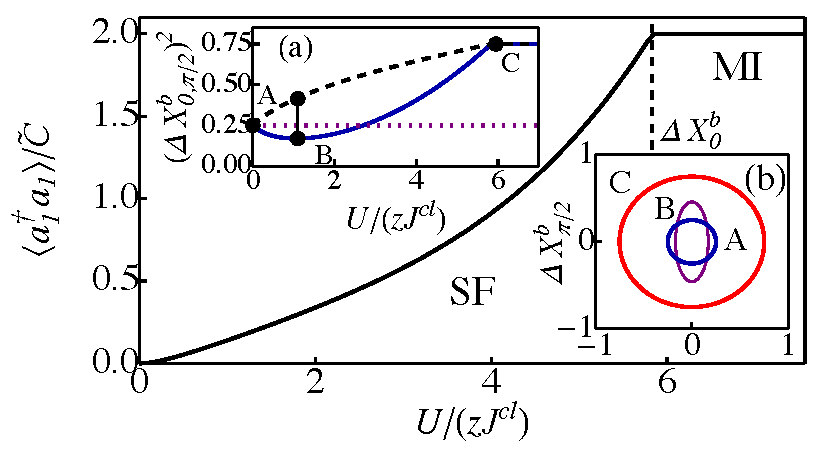
\includegraphics[width=\linewidth]{Quads}
  \captionsetup{justification=centerlast,font=small}
  \caption[Mean-Field Matter Quadratures]{Photon number scattered in a
    diffraction minimum, given by Eq. (\ref{intensity}), where
    $\tilde{C} = 2 |C|^2 (K-1) \mathcal{F}^2 [W_1](\pi/d)$.  More
    light is scattered from a MI than a SF due to the large
    uncertainty in phase in the insulator. (a) The variances of
    quadratures $\Delta X^b_0$ (solid) and $\Delta X^b_{\pi/2}$
    (dashed) of the matter field across the phase transition. Level
    1/4 is the minimal (Heisenberg) uncertainty. There are three
    important points along the phase transition: the coherent state
    (SF) at A, the amplitude-squeezed state at B, and the Fock state
    (MI) at C. (b) The uncertainties plotted in phase space.}
	\label{Quads}
\end{figure}

Probing $\hat{B}^2$ gives us access to kinetic energy fluctuations
with 4-point correlations ($\bd_i b_j$ combined in pairs). Measuring
the photon number variance, which is standard in quantum optics, will
lead up to 8-point correlations similar to 4-point density
correlations \cite{mekhov2007pra}. These are of significant interest,
because it has been shown that there are quantum entangled states that
manifest themselves only in high-order correlations
\cite{kaszlikowski2008}.

Surprisingly, inter-site terms scatter more light from a Mott
insulator than a superfluid Eq. \eqref{intensity}, as shown in
Fig. \eqref{Quads}, although the mean inter-site density
$\langle \hat{n}(\b{r})\rangle $ is tiny in a MI. This reflects a
fundamental effect of the boson interference in Fock states. It indeed
happens between two sites, but as the phase is uncertain, it results
in the large variance of $\hat{n}(\b{r})$ captured by light as shown
in Eq. \eqref{intensity}. The interference between two macroscopic
BECs has been observed and studied theoretically
\cite{horak1999}. When two BECs in Fock states interfere a phase
difference is established between them and an interference pattern is
observed which disappears when the results are averaged over a large
number of experimental realizations. This reflects the large
shot-to-shot phase fluctuations corresponding to a large inter-site
variance of $\hat{n}(\b{r})$. By contrast, our method enables the
observation of such phase uncertainty in a Fock state directly between
lattice sites on the microscopic scale in-situ.

\section{Conclusions}

In summary, we proposed a nondestructive method to probe quantum gases
in an optical lattice. Firstly, we showed that the density-term in
scattering has an angular distribution richer than classical
diffraction, derived generalized Bragg conditions, and estimated
parameters for the only two relevant experiments to date
\cite{weitenberg2011, miyake2011}. Secondly, we proposed how to
measure the matter-field interference by concentrating light between
the sites. This corresponds to interference at the shortest possible
distance in an optical lattice. By contrast, standard destructive
time-of-flight measurements deal with far-field interference and a
relatively near-field one was used in Ref. \cite{miyake2011}. This
defines most processes in optical lattices. E.g. matter-field phase
changes may happen not only due to external gradients, but also due to
intriguing effects such quantum jumps leading to phase flips at
neighbouring sites and sudden cancellation of tunneling
\cite{vukics2007}, which should be accessible by our method. In
mean-field, one can measure the matter-field amplitude (order
parameter), quadratures and squeezing. This can link atom optics to
areas where quantum optics has already made progress, e.g., quantum
imaging \cite{golubev2010, kolobov1999}, using an optical lattice as
an array of multimode nonclassical matter-field sources with a high
degree of entanglement for quantum information processing. Thirdly, we
demonstrated how the method accesses effects beyond mean-field and
distinguishes all the phases in the Mott-superfluid-glass transition,
which is currently a challenge \cite{derrico2014}. Based on
off-resonant scattering, and thus being insensitive to a detailed
atomic level structure, the method can be extended to molecules
\cite{LP2013}, spins, and fermions \cite{ruostekoski2009}.

%%*******************************************************************************
%*********************************** Fourth Chapter *****************************
%*******************************************************************************

\chapter{Quantum Measurement Backaction}  
\label{chap:backaction}
% Title of the Fourth Chapter

\ifpdf
    \graphicspath{{Chapter4/Figs/Raster/}{Chapter4/Figs/PDF/}{Chapter4/Figs/}}
\else
    \graphicspath{{Chapter4/Figs/Vector/}{Chapter4/Figs/}}
\fi


%********************************** %First Section  **************************************

\section{Introduction}

This thesis is entirely concerned with the question of measuring a
quantum many-body system using quantised light. However, so far we
have only looked at expectation values in a nondestructive context
where we neglect the effect of the quantum wave function collapse. We
have shown that light provides information about various statistical
quantities of the quantum states of the atoms such as their
correlation functions. In general, any quantum measurement affects the
system even if it does not physically destroy it. In our model both
optical and matter fields are quantised and their interaction leads to
entanglement between the two subsystems. When a photon is detected and
the electromagnetic wave function of the optical field collapses, the
matter state is also affected due to this entanglement resulting in
quantum measurement backaction. Therefore, in order to determine these
quantities multiple measurements have to be performed to establish a
precise measurement of the expectation value which will require
repeated preparations of the initial state.

In the following chapters, we consider a different approach to quantum
measurement in open systems and instead of considering expectation
values we look at a single experimental run and the resulting dynamics
due to measurement backaction. Previously, we were mostly interested
in extracting information about the quantum state of the atoms from
the scattered light. The flexibility in the measurement model was used
to enable probing of as many different quantum properties of the
ultracold gas as possible. By focusing on measurement backaction we
instead investigate the effect of photodetections on the dynamics of
the many-body gas as well as the possible quantum states that we can
prepare instead of what information can be extracted.

In this chapter, we introduce the necessary theory of quantum
measurement and backaction in open systems in order to lay a
foundation for the material that follows in which we apply these
concepts to a bosonic quantum gas. We first introduce the concept of
quantum trajectories which represent a single continuous series of
photon detections. We also present an alternative approach to open
systems in which the measurement outcomes are discarded. This will be
useful when trying to learn about dynamical features common to every
trajectory. In this case we use the density matrix formalism which
obeys the master equation. This approach is more common in dissipative
systems and we will highlight the differences between these two
different types of open systems. We conclude this chapter with a new
concept that will be central to all subsequent discussions. In our
model measurement is global, it couples to operators that correspond
to global properties of the quantum gas rather than single-site
quantities. This enables the possibility of performing measurements
that cannot distinguish certain sites from each other. Due to a lack
of ``which-way'' information this leads to the creation of spatially
nontrivial virtual lattices on top of the physical lattice. This turns
out to have significant consequences on the dynamics of the system.

\section{Quantum Trajectories}

A simple intuitive concept of a quantum trajectory is that it is the
path taken by a quantum state over time during a single experimental
realisation. In particular, we consider states conditioned upon
measurement results such as the photodetection times. Such a
trajectory is generally stochastic in nature as light scattering is
not a deterministic process. Furthermore, they are in general
discontinuous as each detection event brings about a drastic change in
the quantum state due to the wave function collapse of the light field.

Before we discuss specifics relevant to our model of quantised light
interacting with a quantum gas we present a more general overview
which will be useful as some of the results in the following chapters
are more general. Measurement always consists of at least two
competing processes, two possible outcomes. If there is no competition
and only one outcome is possible then our probe is meaningless as it
does not reveal any information about the system. In its simplest form
measurement consists of a series of detection events, such as the
detections of photons. Even though, on an intuitive level it seems
that we have defined only a single outcome, the detection event, this
arrangement actually consists of two mutually exclusive outcomes. At
any point in time an event either happens or it does not, a photon is
either detected or the detector remains silent, also known as a null
result. Both outcomes reveal some information about the system we are
investigating. For example, let us consider measuring the number of
atoms by measuring the number of photons they scatter. Each atom will
on average scatter a certain number of photons contributing to the
detection rate we observe. Therefore, if we record multiple photons at
a high rate of arrival we learn that the illuminated region must
contain many atoms. On the other hand, if there are few atoms to
scatter the light we will observe few detection events which we
interpret as a continuous series of non-detection events interspersed
with the occasional detector click. This trajectory informs us that
there are much fewer atoms being illuminated than previously.

Basic quantum mechanics tells us that such measurements will in
general affect the quantum state in some way. Each event will cause a
discontinuous quantum jump in the wave function of the system and it
will have a jump operator, $\c$, associated with it. The effect of a
detection event on the quantum state is simply the result of applying
this jump operator to the wave function, $| \psi (t) \rangle$,
\begin{equation}
  \label{eq:jump}
  | \psi(t + \mathrm{d}t) \rangle = \frac{\c | \psi(t) \rangle}
  {\sqrt{\langle \cd \c \rangle (t)}},
\end{equation}
where the denominator is simply a normalising factor
\cite{MeasurementControl}. The exact form of the jump operator $\c$
will depend on the nature of the measurement we are considering. For
example, if we consider measuring the photons escaping from a leaky
cavity then $\c = \sqrt{2 \kappa} \a$, where $\kappa$ is the
cavity decay rate and $\a$ is the annihilation operator of a
photon in the cavity field. It is interesting to note that due to
renormalisation the effect of a single quantum jump is independent of
the magnitude of the operator $\c$ itself. However, larger operators
lead to more frequent events and thus more frequent applications of
the jump operator.

The null measurement outcome will have an opposing effect to the
quantum jump, but it has to be treated differently as it does not
occur at discrete time points like the detection events themselves
\cite{MeasurementControl}. Its effect is accounted for by a
modification to the isolated Hamiltonian, $\hat{H}_0$, time evolution
in the form
\begin{equation}
  | \psi (t + \mathrm{d}t) \rangle = \left\{ \hat{1} - \mathrm{d}t
    \left[ i \hat{H}_0 + \frac{\cd \c}{2} - \frac{\langle \cd \c
        \rangle (t)}{2} \right] \right\} | \psi (t) \rangle.
\end{equation}
The effect of both outcomes can be included in a single stochastic
Schr\"{o}dinger equation given by
\begin{equation}
  \label{eq:SSE}
  \mathrm{d} | \psi(t) \rangle = \left[ \mathrm{d} N(t) \left(
      \frac{\c} {\sqrt{ \langle \cd \c \rangle (t)}} - \hat{1} \right)
    + \mathrm{d} t \left( \frac{\langle \cd \c \rangle (t)}{2} -
      \frac{ \cd \c}{2} - i \hat{H}_0 \right) \right] | \psi(t) \rangle,
\end{equation}
where $\mathrm{d}N(t)$ is the stochastic increment to the number of
photodetections up to time $t$ which is equal to $1$ whenever a
quantum jump occurs and $0$ otherwise \cite{MeasurementControl}. Note
that this equation has a straightforward generalisation to multiple
jump operators, but we do not consider this possibility here at all.

All trajectories that we calculate in the following chapters are
described by the stochastic Schr\"{o}dinger equation in
Eq. \eqref{eq:SSE}. The most straightforward way to solve it is to
replace the differentials by small time-steps $\delta t$. Then we
generate a random number $R(t)$ at every time-step and a jump is
applied, i.e.~$\mathrm{d}N(t) = 1$, if
\begin{equation}
  R(t) < \langle \cd \c \rangle (t) \delta t.
\end{equation}

In practice, this is not the most efficient method for simulation
\cite{MeasurementControl}. Instead we will use the following
method. At an initial time $t = t_0$ a random number $R$ is
generated. We then propagate the unnormalised wave function
$| \tilde{\psi} (t) \rangle$ using the non-Hermitian evolution given
by
\begin{equation}
  \frac{\mathrm{d}}{\mathrm{d}t} | \tilde{\psi} (t) \rangle = -i
  \left( \hat{H}_0 - i \frac{\cd \c}{2} \right) | \tilde{\psi} (t) \rangle
\end{equation}
up to a time $T$ such that
$\langle \tilde{\psi} (T) | \tilde{\psi} (T) \rangle = R$. This
problem can be solved efficiently using standard numerical
techniques. At time $T$ a quantum jump is applied according to
Eq. \eqref{eq:jump} which renormalises the wave function as well and
the process is repeated as long as desired. This formulation also has
the advantage that it provides a more intuitive picture of what
happens during a single trajectory. The quantum jumps are
self-explanatory, but now we have a clearer picture of the effect of
null outcomes on the quantum state. Its effect is entirely encoded in
the non-Hermitian modification to the original Hamiltonian given by
$\hat{H} = \hat{H}_0 - i \cd \c / 2$. It is now easy to see that for a
jump operator, $\c$, with a large magnitude the no-event outcomes will
have a more significant effect on the quantum state. At the same time
they will lead to more frequent quantum jumps which have an opposing
effect to the non-Hermitian evolution, because the jump condition is
satisfied $\langle \tilde{\psi} (T) | \tilde{\psi} (T) \rangle = R$
more frequently. In general, the competition between these two
processes is balanced and without any further external influence the
distribution of outcomes over many trajectories will be entirely
determined by the initial state even though each individual trajectory
will be unique and conditioned on the exact detection times that
occurred during the given experimental run. However, individual
trajectories can have features that are not present after averaging
and this is why we focus our attention on single experimental runs
rather than average behaviour.

\begin{figure}[htbp!]
  \centering
  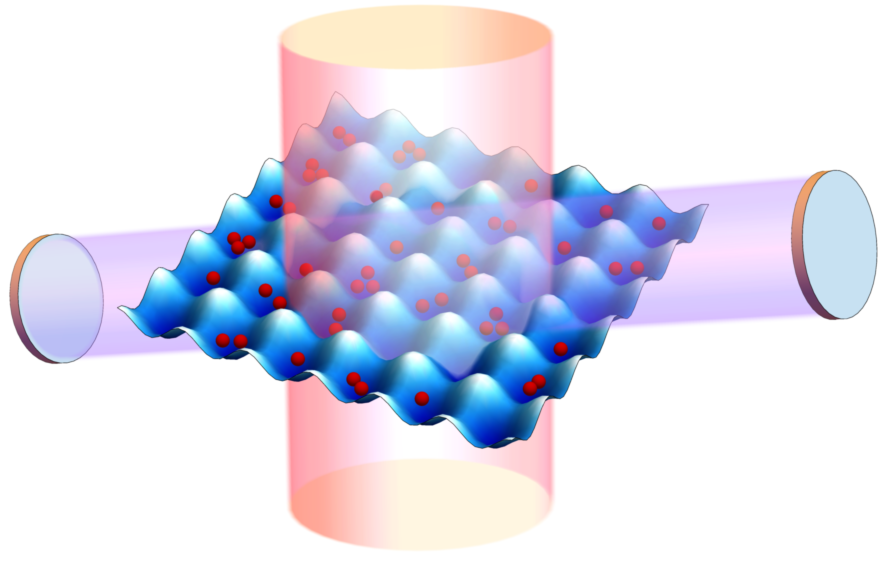
\includegraphics[width=1.0\textwidth]{setup}
  \caption[Experimental Setup with Cavity]{Atoms in an optical lattice
    are probed by a coherent light beam (red), and the light scattered
    (blue) at a particular angle is enhanced and collected by a leaky
    cavity. The photons escaping the cavity are detected, perturbing
    the atomic evolution via measurement backaction.}
  \label{fig:cavity}
\end{figure}

The quantum trajectory theory can now be very straightforwardly
applied to our model of ultracold bosons in an optical
lattice. However, from now on we will only consider the case when the
atomic system is coupled to a single mode cavity in order to enhance
light scattering in one particular direction as shown in
Fig. \ref{fig:cavity}. This way we have complete control over the form
of the quantum jump operator, because light scattering in different
directions corresponds to different measurements as we have seen in
Eq. \eqref{eq:Jcoeff}. On the other hand, in free space we would have
to simultaneously consider all the possible directions in which light
could scatter and thus include multiple jump operators reducing our
ability to control the system.

The model we derived in Eq. \eqref{eq:fullH} is in fact already in a
form ready for quantum trajectory simulations. The phenomenologically
included cavity decay rate $-i \kappa \ad_1 \a_1$ is in fact the
non-Hermitian term $-i \cd \c / 2$, where $\c = \sqrt{2 \kappa} \a_1$
which is the jump operator we want for measurements of photons leaking
from the cavity. However, we will first simplify the system by
considering the regime where we can neglect the effect of the quantum
potential that builds up in the cavity. Physically, this means that
whilst light scatters due to its interaction with matter, the field
that builds up due to the scattered photons collecting in the cavity
has a negligible effect on the atomic evolution compared to its own
dynamics such as inter-site tunnelling or on-site interactions. This
can be achieved when the cavity-probe detuning is smaller than the
cavity decay rate, $\Delta_p \ll \kappa$
\cite{caballero2015}. However, even though the cavity field has a
negligible effect on the atoms, measurement backaction will not. This
effect is of a different nature. It is due to the wave function
collapse due to the destruction of photons rather than an interaction
between fields. Therefore, the final form of the Hamiltonian
Eq. \eqref{eq:fullH} that we will be using in the following chapters
is
\begin{equation}
  \label{eq:backaction}
  \hat{H} = \hat{H}_0 - i \gamma \hat{F}^\dagger \hat{F}
\end{equation}
\begin{equation}
  \hat{H}_0 = -J \sum_{\langle i, j \rangle} \bd_i b_j + \frac{U}{2}
                \sum_i \n_i (\n_i - 1),
\end{equation}
where $\hat{H}_0$ is simply the Bose-Hubbard Hamiltonian,
$\gamma = \kappa |C|^2$ is a quantity that measures the strength of
the measurement and we have substituted $\a_1 = C \hat{F}$. The
quantum jumps are applied at times determined by the algorithm
described above and the jump operator is given by
\begin{equation}
  \label{eq:jumpop}
  \c = \sqrt{2 \kappa} C \hat{F}.
\end{equation}
Importantly, we see that measurement introduces a new energy and time
scale $\gamma$ which competes with the two other standard scales
responsible for the unitary dynamics of the closed system, tunnelling,
$J$, and on-site interaction, $U$.  If each atom scattered light
independently a different jump operator $\c_i$ would be required for
each site projecting the atomic system into a state where long-range
coherence is degraded. This is a typical scenario for spontaneous
emission \cite{pichler2010, sarkar2014}, or for local
\cite{syassen2008, kepesidis2012, vidanovic2014, bernier2014,
  daley2014} and fixed-range addressing \cite{ates2012, everest2014}
which are typically considered in open systems. In contrast to such
situations, we consider global coherent scattering with an operator
$\c$ that is nonlocal. Therefore, the effect of measurement backaction
is global as well and each jump affects the quantum state in a highly
nonlocal way and most importantly not only will it not degrade
long-range coherence, it will in fact lead to such long-range
correlations itself.

In Chapter \ref{chap:qnd} we used highly efficient DMRG methods
\cite{tnt} to calculate the ground state of the Bose-Hubbard
Hamiltonian. Related techniques such as Time-Evolving Block Decimation
(TEBD) or t-DMRG are often used for numerical calculations of time
evolution. However, despite the fact that our Hamiltonian in
Eq. \eqref{eq:backaction} is simply the Bose-Hubbard model with a
non-Hermitian term added due to measurement it is actually difficult
to apply these methods to our system. The problem lies in the fact
that Matrix Product methods we mentioned are only efficient for
one-dimensional systems that obey the area law for entanglement
entropy, i.e.~systems with only short-range quantum
correlations. Unfortunately, the global nature of the measurement we
consider violates the assumptions made in deriving the area law and,
as we shall see in the following chapters, leads to long-range
correlations regardless of coupling strength. Therefore, we resort to
using alternative methods such as exact diagonalisation which we solve
with well-known ordinary differential equation solvers. This means
that we can at most simulate a few atoms, but as we shall see it is
the geometry of the measurement that matters the most and these
effects are already visible in smaller systems.

\section{The Master Equation}
\label{sec:master}

A quantum trajectory is stochastic in nature, it depends on the exact
timings of the quantum jumps which are determined randomly. This makes
it difficult to obtain conclusive deterministic answers about the
behaviour of single trajectories. One possible approach that is very
common when dealing with open systems is to look at the unconditioned
state which is obtained by averaging over the random measurement
results which condition the system \cite{MeasurementControl}. The
unconditioned state is no longer a pure state and thus must be
described by a density matrix,
\begin{equation}
  \label{eq:rho}
  \hat{\rho} = \sum_i p_i | \psi_i \rangle \langle \psi_i |,
\end{equation}
where $p_i$ is the probability the system is in the pure state
$| \psi_i \rangle$. If more than one $p_i$ value is non-zero then the
state is mixed, it cannot be represented by a single pure state. The
time evolution of the density operator obeys the master equation given
by
\begin{equation}
  \dot{\hat{\rho}} = -i \left[ \hat{H}_0, \hat{\rho} \right] + \c
  \hat{\rho} \cd - \frac{1}{2} \left( \cd \c \hat{\rho} + \hat{\rho}
    \cd \c \right).
\end{equation}
Physically, the unconditioned state, $\rho$, represents our knowledge
of the quantum system if we are ignorant of the measurement outcome
(or we choose to ignore it), i.e.~we do not know the timings of the
detection events. 

We will be using the master equation and the density operator
formalism in the context of measurement. However, the exact same
methods are also applied to a different class of open systems, namely
dissipative systems \cite{QuantumNoise}. A dissipative system is an
open system that couples to an external bath in an uncontrolled
way. The behaviour of such a system is similar to a system subject
under observation in which we ignore all the results. One can even
think of this external coupling as a measurement who's outcome record
is not accessible and thus must be represented as an average over all
possible trajectories. However, there is a crucial difference between
measurement and dissipation. When we perform a measurement we use the
master equation to describe system evolution if we ignore the
measurement outcomes, but at any time we can look at the detection times
and obtain a conditioned pure state for this current experimental
run. On the other hand, for a dissipative system we simply have no
such record of results and thus the density matrix predicted by the
master equation, which in general will be a mixed state, represents
our best knowledge of the system. In order to obtain a pure state, it
would be necessary to perform an actual measurement.

A definite advantage of using the master equation for measurement is
that it includes the effect of any possible measurement
outcome. Therefore, it is useful when extracting features that are
common to many trajectories, regardless of the exact timing of the
events. In this case we do not want to impose any specific trajectory
on the system as we are not interested in a specific experimental run,
but we would still like to identify the set of possible outcomes and
their common properties. Unfortunately, calculating the inverse of
Eq. \eqref{eq:rho} is not an easy task. In fact, the decomposition of
a density matrix into pure states might not even be unique. However,
if a measurement leads to a projection, i.e.~the final state becomes
confined to some subspace of the Hilbert space, then this will be
visible in the final state of the density matrix. We will show this on
an example of a qubit in the quantum state
\begin{equation}
  \label{eq:qubit0}
  | \psi \rangle = \alpha |0 \rangle + \beta | 1 \rangle,
\end{equation}
where $| 0 \rangle$ and $| 1 \rangle$ represent the two basis states
of the qubit and we consider performing a measurement in the basis
$\{| 0 \rangle, | 1 \rangle \}$, but we don't check the outcome.  The
quantum state will have collapsed now to the state $ | 0 \rangle$ with
probability $| \alpha |^2$ and $| 1 \rangle$ with probability
$| \beta |^2$. The corresponding density matrix is given by
\begin{equation}
  \label{eq:rho1}
  \hat{\rho} = \left( \begin{array}{cc}
                        | \alpha |^2 & 0 \\
                        0 & |\beta|^2 
                      \end{array} \right),
\end{equation}
which is a mixed state as opposed to the initial state. We note that
there are no off-diagonal terms as the system is not in a
superposition between the two basis states. Therefore, the diagonal
terms represent classical probabilities of the system being in either
of the basis states. This is in contrast to their original
interpretation when the state was given by Eq. \eqref{eq:qubit0} when
they could not be interpreted as in such a way. The initial state was
in a quantum superposition and thus the state was indeterminate due to
the quantum uncertainty in our knowledge of the state which would have
manifested itself in the density matrix as non-zero off-diagonal
terms. The significance of these values being classical probabilities
is that now we know that the measurement has already happened and we
know with certainty that the state must be either $| 0 \rangle$ or
$| 1 \rangle$. We just don't know which one until we check the result
of the measurement.

We have assumed that it was a discrete wave function collapse that lead
to the state in Eq. \eqref{eq:rho1} in which case the conclusion we
reached was obvious. However, the nature of the process that takes us
from the initial state to the final state with classical uncertainty
does not matter. The key observation is that regardless of the
trajectory taken, if the final state is given by Eq. \eqref{eq:rho1}
we will definitely know that our state is either in the state
$| 0 \rangle$ or $| 1 \rangle$ and not in some superposition of the
two basis states. Therefore, if we obtained this density matrix as a
result of applying the time evolution given by the master equation we
would be able to identify the final states of individual trajectories
even though we have no information about the individual trajectories
themselves. This is analogous to an approach in which decoherence due to
coupling to the environment is used to model the wave function collapse
\cite{zurek2002}, but here we will be looking at projective effects
due to weak measurement.

Here we have considered a very simple case of a Hilbert space with two
non-degenerate basis states. In the following chapters we will
generalise the above result to larger Hilbert spaces with multiple
degenerate subspaces which are of much greater interest as they reveal
nontrivial dynamics in the system.

\section[Global Measurement and ``Which-Way'' Information]
        {Global Measurement and ``Which-Way'' Information\footnote{The
            results of this section were first published in
            Ref. \cite{elliott2015}}}
\label{sec:modes}

We have already mentioned that one of the key features of our model is
the global nature of the measurement operators. A single light mode
couples to multiple lattice sites from where atoms scatter the light
coherently into a single mode which we enhance and collect with a
cavity. If atoms at different lattice sites scatter light with a
different phase or magnitude we will be able to identify which atoms
contributed to the light we detected. However, if they scatter the
photons in phase and with the same amplitude then we have no way of
knowing which atom emitted the photon, we have no ``which-way''
information. When we were considering nondestructive measurements and
looking at expectation values, this had no consequence on our results
as we were simply interested in probing the quantum correlations of a
given ground state and whether two sites were distinguishable or not
was irrelevant. Now, on the other hand, we are interested in the
effect of these measurements on the dynamics of the system. The effect
of measurement backaction will depend on the information that is
encoded in the detected photon. If a scattered mode cannot
distinguish between two different lattice sites then we have no
information about the distribution of atoms between those two sites.
Therefore, all quantum correlations between the atoms in these sites
are unaffected by the backaction whilst their correlations with the
rest of the system will change as the result of the quantum jumps.

\begin{figure}[htbp!]
  \centering
  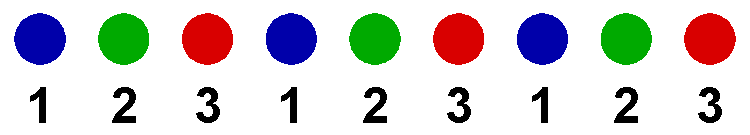
\includegraphics[width=1.0\textwidth]{1DModes}
  \caption[1D Modes due to Measurement Backaction]{The coefficients,
    and thus the operator $\hat{D}$ is made periodic with a period of
    three lattice sites. Therefore, the coefficients $J_{i,i}$ will
    repeat every third site making atoms in those sites
    indistinguishable to the measurement. Physically, this is due to
    the fact that this periodic arrangement causes the atoms within a
    single mode to scatter light with the same phase and amplitude.
    The scattered light contains no information which can be used to
    determine the atom distribution.}
  \label{fig:1dmodes}
\end{figure}

The quantum jump operator for our model is given by
$\c = \sqrt{2 \kappa} C \hat{F}$ and we know from Eq. \eqref{eq:F}
that we have a large amount of flexibility in tuning $\hat{F}$ via the
geometry of the optical setup. A cavity aligned at a different angle
will correspond to a different measurement. We will consider the case
when $\hat{F} = \hat{D}$ given by Eq. \eqref{eq:D}, but since the
argument depends on geometry rather than the exact nature of the
operator it straightforwardly generalises to other measurement
operators, including the case when $\hat{F} = \hat{B}$ where the bonds
(inter-site operators) play the role of lattice sites. The operator
$\hat{D}$ is given by
\begin{equation}
  \hat{D} = \sum_i J_{i,i} \n_i,
\end{equation}
where the coefficients $J_{i,i}$ are determined from
Eq. \eqref{eq:Jcoeff}. These coefficients represent the coupling
strength between the atoms and the light modes and thus their spatial
variation can be easily tuned by the geometry of the optical
fields. We are in particular interested in making these coefficients
degenerate across a number of lattice sites as shown in
Figs. \ref{fig:1dmodes} and \ref{fig:2dmodes}. Note that they do not
have to be periodic, but it is much easier to make them so. This makes
all lattice sites with the same value of $J_{i,i}$ indistinguishable
to the measurement thus partitioning the lattice into a number of
distinct zones which we will refer to as modes. It is crucial to note
that these partitions in general are not neighbours of each other,
they are not localised, they overlap in a nontrivial way, and the
patterns can be made more complex in higher dimensions as shown in
Fig. \ref{fig:2dmodes} or with a more sophisticated optical setup
\cite{caballero2016}. This has profound consequences as it can lead to
the creation of long-range nonlocal correlations between lattice sites
\cite{mazzucchi2016, kozlowski2016zeno}. The measurement does not know
which atom within a certain mode scattered the light, there is no
``which-way'' information. Therefore, from the point of view of the
observer's knowledge all atoms within a mode are identical regardless
of their spatial separation. This effect can be used to create virtual
lattices on top of the physical lattice.

\begin{figure}[htbp!]
  \centering
  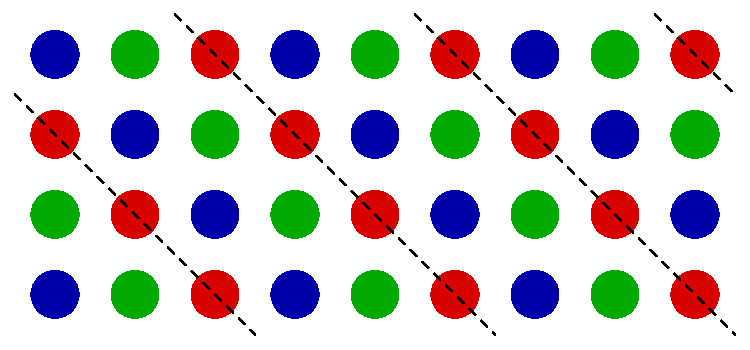
\includegraphics[width=1.0\textwidth]{2DModes}
  \caption[2D Modes due to Measurement Backaction]{ More complex
    patterns of virtual lattice can be created in higher
    dimensions. With a more complicated setup even more complicated
    geometries are possible.}
  \label{fig:2dmodes}
\end{figure}

We will now look at a few practical examples.  The simplest case is to
measure in the diffraction maximum such that $\a_1 = C \hat{N}_K$,
where $\hat{N}_K = \sum_j^K \hat{n}_j$ is the number of atoms in the
illuminated area. If the whole lattice is illuminated we effectively
have a single mode as $J_{i,i} = 1$ for all sites. If only a subset of
lattice sites is illuminated $K < M$ then we have two modes
corresponding to the illuminated and unilluminated sites. It is
actually possible to perform such a measurement in a nonlocal way by
arranging every other site (e.g.~all the even sites) to be at a node
of both the cavity and the probe. The resulting field measures the
number of atoms in the remaining sites (all the odd sites) in a global
manner. It does not know how these atoms are distributed among these
sites as we do not have access to the individual sites. This two mode
arrangement is shown in the top panel of Fig. \ref{fig:twomodes}. A
different two-mode arrangement is possible by measuring in the
diffraction minimum such that each site scatters in anti-phase with
its neighbours as shown in the bottom panel of
Fig. \ref{fig:twomodes}. 

\begin{figure}[htbp!]
  \centering
  
\includegraphics[width=0.7\textwidth]{TwoModes1}
  
\includegraphics[width=0.7\textwidth]{TwoModes2}
  \caption[Two Mode Partitioning]{Top: only the odd sites scatter
    light leading to a measurement of $\hat{N}_\mathrm{odd}$ and an
    effective partitioning into even and odd sites. Bottom: this also
    partitions the lattice into odd and even sites, but this time
    atoms at all sites scatter light, but in anti-phase with their
    neighbours.}
  \label{fig:twomodes}
\end{figure}

This approach can be generalised to an arbitrary number of modes,
$Z$. For this we will consider a deep lattice such that
$J_{i,i} = u_1^* (\b{r}) u_0 (\b{r})$. We will take the probe beam to
be incident normally at a 1D lattice so that $u_0 (\b{r}) =
1$. Therefore, the final form of the scattered light field is given by
\begin{equation}
  \label{eq:Dmodes}
  \a_1 = C \hat{D} = C \sum_m^K \exp\left[-i k_1 m d \sin \theta_1
  \right] \hat{n}_m.
\end{equation}
From this equation we see that it can be made periodic with a period
$Z$ when
\begin{equation}
  k_1 d \sin \theta_1 = 2\pi R / Z,
\end{equation}
where $R$ is just some integer and $R/Z$ are is a fraction in its
simplest form. Therefore, we can rewrite the Eq. \eqref{eq:Dmodes} as
a sum of the indistinguishable contributions from the $Z$ modes
\begin{equation}
  \label{eq:Zmodes}
  \a_1 = C \hat{D} = C \sum_l^Z \exp\left[-i 2 \pi l R / Z \right] \hat{N}_l,
\end{equation}
where $\hat{N}_l = \sum_{m \in l} \n_m$ is the sum of single site atom
number operators that belong to the same mode. $\hat{N}_K$ and
$\hat{N}_\mathrm{odd}$ are the simplest examples of these modes. This
partitions the 1D lattice in exactly $Z > 1$ modes by making every
$Z$th lattice site scatter light with exactly the same phase. It is
interesting to note that these angles correspond to the $K-1$
classical diffraction minima.


%%*******************************************************************************
%*********************************** Fifth Chapter *****************************
%*******************************************************************************

\chapter{Density Measurement Induced Dynamics}
% Title of the Fifth Chapter

\ifpdf
    \graphicspath{{Chapter5/Figs/Raster/}{Chapter5/Figs/PDF/}{Chapter5/Figs/}}
\else
    \graphicspath{{Chapter5/Figs/Vector/}{Chapter5/Figs/}}
\fi


\section{Introduction}

In the previous chapter we have introduced a theoretical framework
which will allow us to study measurement backaction using
discontinuous quantum jumps and non-Hermitian evolution due to null
outcomesquantum trajectories. We have also wrapped our quantum gas
model in this formalism by considering ultracold bosons in an optical
lattice coupled to a cavity which collects and enhances light
scattered in one particular direction. One of the most important
conclusions of the previous chapter was that the introduction of
measurement introduces a new energy and time scale into the picture
which competes with the intrinsic dynamics of the bosons.

In this chapter, we investigate the effect of quantum measurement
backaction on the many-body state and dynamics of atoms. In
particular, we will focus on the competition between the backaction
and the the two standard short-range processes, tunnelling and on-site
interactions, in optical lattices. We show that the possibility to
spatially structure the measurement at a microscopic scale comparable
to the lattice period without the need for single site resolution
enables us to engineer efficient competition between the three
processes in order to generate new nontrivial dynamics. However,
unlike tunnelling and on-site interactions our measurement scheme is
global in nature which makes it capable of creating long-range
correlations which enable nonlocal dynamical processes. Furthermore,
global light scattering from multiple lattice sites creates nontrivial
spatially nonlocal coupling to the environment which is impossible to
obtain with local interactions \cite{daley2014, diehl2008,
  syassen2008}. These spatial modes of matter fields can be considered
as designed systems and reservoirs opening the possibility of
controlling dissipations in ultracold atomic systems without resorting
to atom losses and collisions which are difficult to manipulate. Thus
the continuous measurement of the light field introduces a
controllable decoherence channel into the many-body dynamics. Such a
quantum optical approach can broaden the field even further allowing
quantum simulation models unobtainable using classical light and the
design of novel systems beyond condensed matter analogues.

In the weak measurement limit, where the quantum jumps do not occur
frequently compared to the tunnelling rate, this can lead to global
macroscopic oscillations of bosons between odd and even sites. These
oscillations occur coherently across the whole lattice enabled by the
fact that measurement is capable of generating nonlocal spatial
modes. When on-site interactions are included we obtain a system with
three competing energy scales of which two correspond to local
processes and one is global. This complicates the picture
immensely. We show how under certain circumstances interactions
prevent measurement from generating globally coherent dynamics, but on
the other hand when the measurement is strong both processes
collaborate in squeezing the atomic distribution.

On the other end of the spectrum, when measurement is strong we enter
the regime of quantum Zeno dynamics. Frequent measurements can slow
the evolution of a quantum system leading to the quantum Zeno effect
where a quantum state is frozen in its initial configuration
\cite{misra1977, facchi2008}. One can also devise measurements with
multi-dimensional projections which lead to quantum Zeno dynamics
where unitary evolution is uninhibited within this degenerate
subspace, usually called the Zeno subspace \cite{facchi2008,
  raimond2010, raimond2012, signoles2014}. Our flexible setup where global light
scattering can be engineered allows us to suppress or enhance specific
dynamical processes thus realising spatially nonlocal quantum Zeno
dynamics. This unconventional variation occurs when measurement is
near, but not in, its projective limit. The system is still confined
to Zeno subspaces, but intermediate transitions are allowed via
virtual Raman-like processes. We show that this result can, in general
(i.e.~beyond the ultracold gas model), be approximated by a
non-Hermitian Hamiltonian thus extending the notion of quantum Zeno
dynamics into the realm of non-Hermitian quantum mechanics joining the
two paradigms.

\section{Quantum Measurement Induced Dynamics}

\subsection{Large-Scale Dynamics due to Weak Measurement}

We start by considering the weak measurement limit when photon
scattering does not occur frequently compared to the tunnelling rate
of the atoms, i.e.~$\gamma \ll J$. When the system is probed in this
way, the measurement is unable to project the quantum state of the
bosons to an eigenspace as postulated by the Copenhagen interpretation
of quantum mechanics. The backaction of the photodetections is simply
not strong or frequent enough to confine the atoms. However, instead
of confining the evolution of the quantum state, it has been shown in
Refs. \cite{mazzucchi2016, mazzucchi2016njp} that the measurement
leads to coherent global oscillations between the modes generated by
the spatial profile of the light field which we have seen in section
\ref{sec:modes}. Fig. \ref{fig:oscillations} illustrates the atom
number distributions in the odd sites for $Z = 2$ and one of the three
modes for $Z = 3$. These oscillations correspond to atoms flowing from
one mode to another. We only observe a small number of well defined
components which means that this flow happens in phase, all the atoms
are tunnelling between the modes together in unison. Furthermore, this
exchange of population is macroscopic in scale. The trajectories reach
a state where the maximum displacement point corresponds to all the
atoms being entirely within a single mode. Finally, we note that these
oscillating distributions are squeezed by the measurement and the
individual components have a width smaller than the initial state. By
contrast, in the absence of the external influence of measurement
these distributions would spread out significantly and the center of
the broad distribution would oscillate with an amplitude comparable to
the initial imbalance, i.e.~small oscillations for a small initial
imbalance.

\begin{figure}[htbp!]
  \centering
  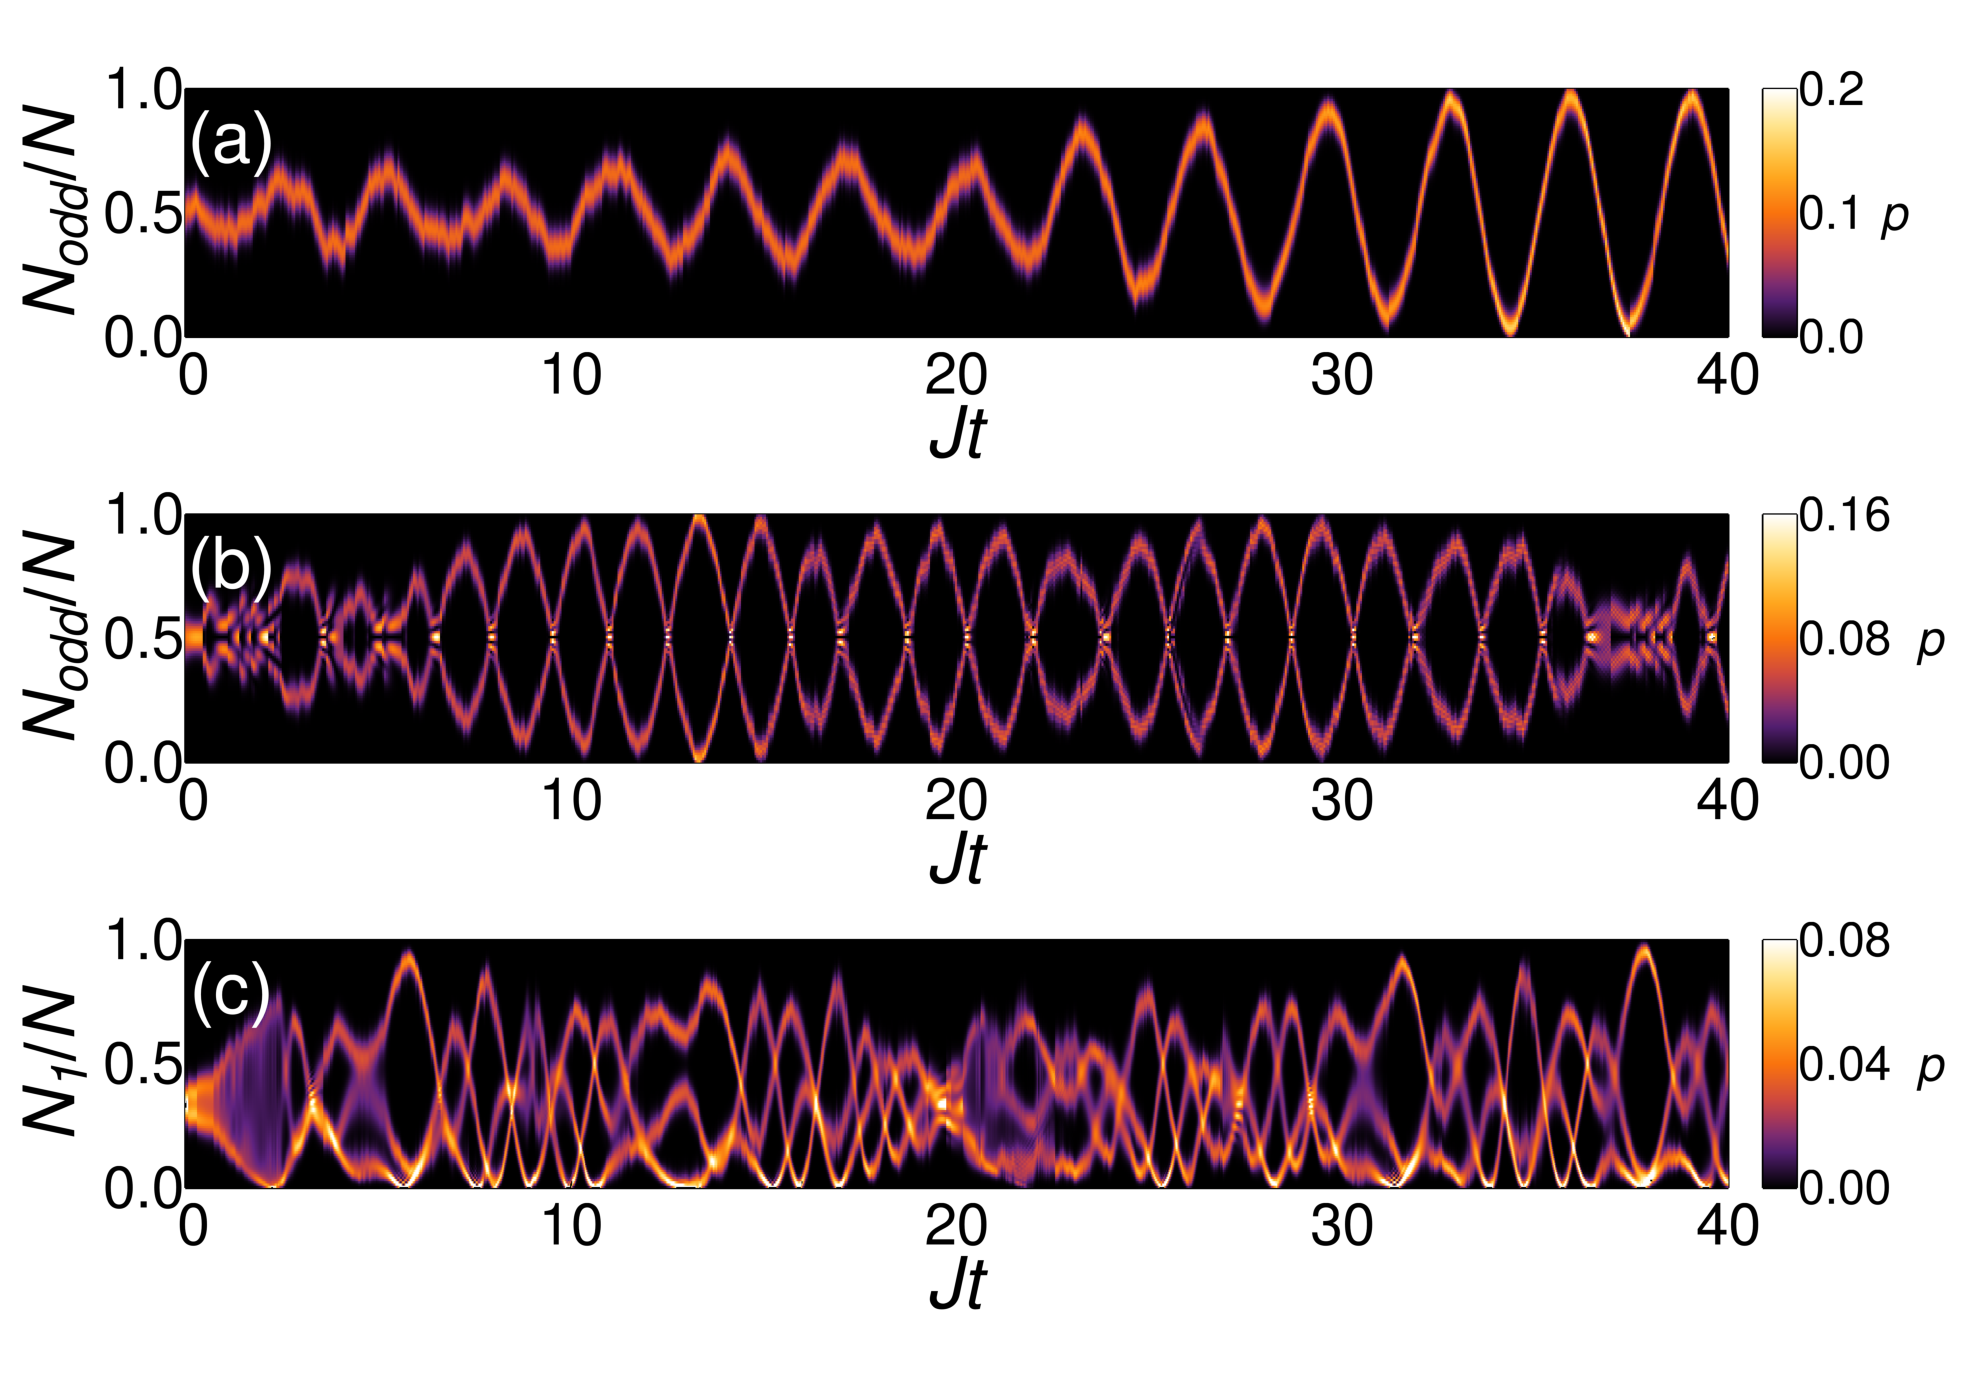
\includegraphics[width=\textwidth]{Oscillations}
  \caption[Macroscopic Oscillations due to Weak Measurement]{Large
    oscillations between the measurement-induced spatial modes
    resulting from the competition between tunnelling and weak
    measurement induced backaction. The plots show the atom number
    distributions $p(N_l)$ in one of the modes in individual quantum
    trajectories. These dstributions show various numbers of
    well-squeezed components reflecting the creation of macroscopic
    superposition states depending on the measurement
    configuration. $U/J = 0$, $\gamma/J = 0.01$, $M=N$, initial
    states: bosonic superfluid. (a) Measurement of the atom number at
    odd sites $\hat{N}_\mathrm{odd}$ creates one strongly oscillating
    component in $p(N_\mathrm{odd})$ ($N = 100$ bosons, $J_{j,j} = 1$
    if $j$ is odd and 0 otherwise). (b) Measurement of
    $(\hat{N}_\mathrm{odd} - \hat{N}_\mathrm{even})^2$ introduces
    $Z = 2$ modes and preserves the superposition of positive and
    negative atom number differences in $p(N_\mathrm{odd})$ ($N = 100$
    bosons, $J_{j,j} = (-1)^{j+1}$). (c) Measurement for $Z = 3$ modes
    preserves three components in $p(N_1)$ ($N = 108$ bosons,
    $J_{j,j} = e^{i 2 \pi j / 3}$).}
  \label{fig:oscillations}
\end{figure}

In Figs. \ref{fig:oscillations}(b,c) we also see that the system is
composed of multiple components. This depends on the quantity that is
being measured and it is a consequence of the fact that the detected
light intensity $\ad_1 \a_1$ is not sensitive to the light phase. The
measurement will not distinguish between permutations of mode
occupations that scatter light with the same intensity, but with a
different phase. For example, when measuring
$\hat{D} = \hat{N}_\mathrm{odd} - \hat{N}_\mathrm{even}$, the light
intensity will be proportional to
$\hat{D}^\dagger \hat{D} = (\hat{N}_\mathrm{odd} -
\hat{N}_\mathrm{even})^2$ and thus it cannot distinguish between a
positive and negative imbalance leading to the two components seen in
Fig. \ref{fig:oscillations}. More generally, the number of components
of the atomic state, i.e.~the degeneracy of $\ad_1 \a_1$, can be
computed from the eigenvalues of Eq. \eqref{eq:Zmodes},
\begin{equation}
  \hat{D} = \sum_l^Z \exp\left[-i 2 \pi l R / Z \right] \hat{N}_l.
\end{equation}
Each eigenvalue can be represented as the sum of the individual terms
in teh above sum which are vectors on the complex plane with phases
that are integer multiples of $2 \pi / Z$: $N_1 e^{-i 2 \pi R / Z}$,
$N_2 e^{-i 4 \pi R / Z}$, ..., $N_Z$. Since the set of possible sums
of these vectors is invariant under rotations by $2 \pi l R / Z$,
$l \in \mathbb{Z}$, and reflection in the real axis, the state of the
system is 2-fold degenerate for $Z = 2$ (reflections leave $Z = 2$
unchanged) and $2Z$-fold degenerate for $Z >
2$. Fig. \ref{fig:oscillations} shows the three mode case, where there
are in fact $6$ components ($2Z = 6$), but in this case they all occur
in pairs resulting in only three visible components.

We will now limit ourselves to a specific illumination pattern with
$\hat{D} = \hat{N}_\mathrm{odd}$ as this leads to the simplest
multimode dynamics with $Z = 2$ and only a single component as seen in
Fig. \ref{fig:oscillations}a, i.e.~no multiple peaks like in
Figs. \ref{fig:oscillations}(b,c). This pattern can be obtained by
crossing two beams such that their projections on the lattice are
identical and the even sites are positioned at their nodes. However,
even though this is the simplest possible case and we are only dealing
with non-interacting atoms solving the full dynamics of the
Bose-Hubbard Hamiltonian combined with measurement is nontrivial. The
backaction introduces a highly nonlinear global term. However, it has
been shown in Ref. \cite{mazzucchi2016njp} that the non-interacting
dynamics with quantum measurement backaction for $Z$-modes reduce to
an effective Bose-Hubbard Hamiltonian with $Z$-sites provided the
initial state is a superfluid. In this simplified model the $N_j$
atoms in the $j$-th site correspond to a superfluid of $N_j$ atoms
within a single spatial mode as defined in section
\ref{sec:modes}. Therefore, we now proceed to study the dynamics for
$\hat{D} = \hat{N}_\mathrm{odd}$ using this reduced effective
double-well model.

The atomic state can be written as
\begin{equation}
  \label{eq:discretepsi}
  | \psi \rangle = \sum_l^N q_l |l, N - l \rangle,
\end{equation}
where the ket $| l, N - l \rangle$, represents a superfluid with $l$
atoms in the odd sites and $N-l$ atoms in the even sites. The
non-Hermitian Hamiltonian describing the time evolution in between the
jumps is given by
\begin{equation}
  \label{eq:doublewell}
  \hat{H} = -J^\mathrm{cl} \left( \bd_o b_e + b_o \bd_e \right) - i
  \gamma \n_o^2
\end{equation}
and the quantum jump operator which is applied at each photodetection
is $\c = \sqrt{2 \kappa} C \n_o$. $b_o$ ($\bd_o$) is the annihilation
(creation) operator in the left site of the effective double-well
corresponding to the superfluid at odd sites of the physical
lattice. $b_e$ ($\bd_e$) is defined similarly, but for the right site
and the superfluid at even sites of the physical lattice.
$\n_o = \bd_o b_o$ is the atom number operator in the left site.

Even though Eq. \eqref{eq:doublewell} is relatively simple as it it is
only a non-interacting two-site model, the non-Hermitian term
complicates the situation making the system difficult to
solve. However, a semiclassical approach to boson dynamics in a
double-well in the limit of many atoms $N \gg 1$ has been developed in
Ref. \cite{juliadiaz2012}. It was originally formulated to treat
squeezing in a weakly interacting bosonic gas, but it can easily be
applied to our system as well. In the limit of large atom number, the
wavefunction in Eq. \eqref{eq:discretepsi} can be described using
continuous variables by defining $\psi (x = l / N) = \sqrt{N}
q_l$. Note that this requires the coefficients $q_l$ to vary smoothly
which is the case for a superfluid state. We now rescale the
Hamiltonian in Eq. \eqref{eq:doublewell} to be dimensionless by
dividing by $NJ^\mathrm{cl}$ and define the relative population
imbalance between the two wells $z = 2x - 1$. Finally, by taking the
expectation value of the Hamiltonian and looking for the stationary
points of
$\langle \psi | \hat{H} | \psi \rangle - E \langle \psi | \psi
\rangle$ we obtain the semiclassical Schr\"{o}dinger equation
\begin{equation}
  \label{eq:semicl}
  i h \partial_t \psi(z, t) = \mathcal{H} \psi(z, t),
\end{equation}
\begin{equation}
  \label{eq:semiH}
  \mathcal{H} \approx -2 h^2 \partial^2_z \psi(z, t) + \left[
    \frac{\omega^2 z^2} {8} - \frac{i \Gamma} {4} \left( z + 1
    \right)^2 \right] \psi(z, t),
\end{equation}
where $\Gamma = N \kappa |C|^2 / J$, $h = 1/N$,
$\omega = 2 \sqrt{1 + \Lambda - h}$, and
$\Lambda = NU / (2J^\mathrm{cl})$. The full derivation is not
straightforward, but the introduction of the non-Hermitian term
requires only a minor modification to the original formalism presented
in detail in Ref. \cite{juliadiaz2012} so we have omitted it here. We
will also be considering $U = 0$ as the effective model is only valid
in this limit, thus $\Lambda = 0$. However, this model is valid for an
actual physical double-well setup in which case interacting bosons can
also be considered. The equation is defined on the interval
$z \in [-1, 1]$, but $z \ll 1$ has been assumed in order to simplify
the kinetic term and approximate the potential as parabolic. This does
mean that this approximation is not valid for the maximum amplitude
oscillations seen in Fig. \ref{fig:oscillations}a, but since they
already appear early on in the trajectory we are able to obtain a
valid analytic description of the oscillations and their growth.

A superfluid state in our continuous variable approximation
corresponds to a Gaussian wavefunction $\psi$. Furthermore, since the
potential is parabolic, even with the inclusion of the non-Hermitian
term, it will remain Gaussian during subsequent time
evolution. Therefore, we will use a very general Gaussian wavefunction
of the form
\begin{equation}
  \label{eq:ansatz}
  \psi(z, t) = \frac{1}{\pi b^2}\exp\left[ i \epsilon 
  - \frac{(z - z_0)^2} {2 b^2} + \frac{i \phi (z - z_\phi)^2} {2 b^2} \right]
\end{equation}
as our ansatz to Eq. \eqref{eq:semicl}. The parameters $b$, $\phi$,
$z_0$, and $z_\phi$ are real-valued functions of time whereas
$\epsilon$ is a complex-valued function of time. Physically, the value
$b^2$ denotes the width, $z_0$ the position of the center, $\phi$ and
$z_\phi$ contain the local phase information, and $\epsilon$ only
affects the global phase and norm of the Gaussian wave packet.

The non-Hermitian Hamiltonian and an ansatz are not enough to describe
the full dynamics due to measurement. We also need to know the effect
of each quantum jump. Within the continuous variable approximation,
our quantum jump become $\c \propto 1 + z$. We neglect the constant
prefactors, because the wavefunction is normalised after a quantum
jump. Expanding around the peak of the Gaussian ansatz we get
\begin{equation}
  1 + z \approx \exp \left[ \ln (1 + z_0) + \frac{z - z_0}{1 + z_0} -
    \frac{(z - z_0)^2}{2 (1 + z_0)^2} \right].
\end{equation}
Multiplying the wavefunction in Eq. \eqref{eq:ansatz} with the jump
operator above yields a Gaussian wavefunction as well, but the
parameters change discontinuously according to
\begin{align}
  \label{eq:jumpb2}
  b^2 & \rightarrow \frac{ b^2 (1 + z_0)^2 } { (1 + z_0)^2 + b^2 }, \\
  \phi & \rightarrow \frac{ \phi (1 + z_0)^2 } { (1 + z_0)^2 + b^2 }, \\
  \label{eq:jumpz0}
  z_0 & \rightarrow z_0 + \frac{ b^2 (1 + z_0) } { (1 + z_0)^2 + b^2}, \\
  z_\phi & \rightarrow z_\phi, \\
  \epsilon & \rightarrow \epsilon.
\end{align}
The fact that the wavefunction remains Gaussian after a photodetection
is a huge advantage, because it means that the combined time evolution
of the system can be described with a single Gaussian ansatz in
Eq. \eqref{eq:ansatz} subject to non-Hermitian time evolution
according to Eq. \eqref{eq:semicl} with discontinous changes to the
parameter values at each quantum jump.

Having identified an appropriate ansatz and the effect of quantum
jumps we proceed with solving the dynamics of wavefunction in between
the photodetecions. The initial values of the parameters for a
superfluid state of $N$ atoms across the whole lattice are $b^2 = 2h$,
$\phi =0$, $a_0 = 0$, $a_\phi = 0$, $\epsilon = 0$. However, we use
the most general initial conditions at time $t = t_0$ which we denote
by $b(t_0) = b_0$, $\phi(t_0) = \phi_0$, $z_0(t_0) = a_0$,
$z_\phi(t_0) = a_\phi$, and $\epsilon(t_0) = \epsilon_0$. The reason
for keeping them as general as possible is that after every quantum
jump the system changes discontinuously. The subsequent time evolution
is obtained by solving the Schr\"{o}dinger equation with the post-jump
paramater values as the new initial conditions.

By plugging the ansatz in Eq. \eqref{eq:ansatz} into the
Schr\"{o}dinger equation in Eq. \eqref{eq:semicl} we obtain three
differential equations
\begin{equation}
  \label{eq:p}
  -2 h^2 p^2 + \left( \frac{ \omega^2 } { 8 } - \frac{ i \Gamma } { 4
    } \right) + \frac{ i h } { 2 } \frac{ \mathrm{d} p } { \mathrm{d}
    t } = 0,
\end{equation}
\begin{equation}
  \label{eq:pq}
  4 h^2 p q - \frac{ i \Gamma } { 2 } - i h \frac{ \mathrm{d} q } {
    \mathrm{d} t } = 0
\end{equation}
\begin{equation}
  \label{eq:pqr}
  -2 h^2 (q^2 - p) - \frac{ i \Gamma } { 4 } - i h \left( \frac{ 1 } {
      4 x } \frac{ \mathrm{d} x } {\mathrm{d} t } + i \frac{
      \mathrm{d} \epsilon } { \mathrm{d} t } - \frac{1}{2} \frac{
      \mathrm{d} r } { \mathrm{d} t } \right) = 0,
\end{equation}
where $x = 1/b^2$, $p = (1 - i \phi)/b^2$,
$q = (z_0 - i \phi z_\phi)/b^2$, and
$r = (z_0^2 - \phi z_\phi^2)/b^2$. The corresponding initial
conditions are $x(t_0) = x_0 = 1/b_0^2$,
$p(t_0) = p_0 = (1 - i \phi_0)/b_0^2$,
$q(t_0) = q_0 = (a_0 - \phi_0 a_\phi)/b_0^2$, and
$r(t_0) = r_0 = (a_0^2 - \phi_0 a_\phi^2)/b_0^2$. The original
parameters can be extracted from these auxiliary variables by
$b^2 = 1 / \Re \{ p \}$, $\phi = - \Im \{ p \} / \Re \{ p \}$,
$z_0 = \Re \{ q \} / \Re \{ p \}$,
$z_\phi = \Im \{ q \} / \Im \{ p \}$, and $\epsilon$ appears
explicitly in the equations above.

First, it is worth noting that all parameters of interest can be
extracted from $p(t)$ and $q(t)$ alone. We are not interested in
$\epsilon$ as it is only related to the global phase and the norm of
the wavefunction and it contains little physical
information. Furthermore, an interesting and incredibly convenient
feature of these equations is that the Eq. \eqref{eq:p} is a function
of $p(t)$ alone and Eq. \eqref{eq:pq} is a function of $p(t)$ and
$q(t)$ only. Therefore, we only need to solve first two equations and
we can neglect Eq. \eqref{eq:pqr}. However, in order to actually
perform Monte-Carlo simulations of quantum trajectories
Eq. \eqref{eq:pqr} would need to be solved in order to obtain correct
jump statistics.

We start with Eq. \eqref{eq:p} and we note it can be rearranged into
the form
\begin{equation}
  \frac{ \mathrm{d} p } { (\zeta \omega / 4 h)^2 - p^2 } = i 4 h
  \mathrm{d} t,
\end{equation}
where $\zeta^2 = (\alpha - i \beta)^2 = 1 - i 2 \Gamma / \omega^2$, and
\begin{equation}
  \alpha = \sqrt{ \frac{1}{2} + \frac{1}{2} \sqrt{1 + \frac{ 4\Gamma^2
      }{ \omega^4 }}},
\end{equation}
\begin{equation}
  \beta = -\sqrt{ -\frac{1}{2} + \frac{1}{2} \sqrt{1 + \frac{ 4\Gamma^2
      }{ \omega^4 }}}.
\end{equation}
This is a standard integral\footnotemark and thus yields
\begin{equation}
  \label{eq:psol}
  p(t) = \frac{ \zeta \omega } { 4 h } 
  \frac{ ( \zeta \omega + 4 h p_0 )e^{i \zeta \omega t} - ( \zeta
    \omega - 4 h p_0 ) e^{-i \zeta \omega t} }
  { ( \zeta \omega + 4 h p_0 )e^{i \zeta \omega t} + ( \zeta \omega
    - 4 h p_0 ) e^{-i \zeta \omega t} }.
\end{equation}

\footnotetext{ \[ \int \frac{\mathrm{d} x}{a^2 - x^2} = \frac{1}{2a}
    \ln \left( \frac{a+x}{a-x} \right) + \mathrm{const.} 
    \quad\quad\quad\quad\quad\quad\quad\quad\quad\quad\quad\quad\quad\quad\quad
    \quad\quad\quad\quad\quad\] }

Having found an expression for $p(t)$ we can now solve
Eq. \eqref{eq:pq} for $q(t)$. To do that we first define the
integrating factor
\begin{equation}
  I(t) = \exp \left[ i 4 h \int p \mathrm{d} t \right] = ( \zeta
  \omega + 4 h p_0 )e^{i \zeta \omega t} + ( \zeta \omega - 4 h p_0 )
  e^{-i \zeta \omega t},
\end{equation}
which lets us rewrite Eq. \eqref{eq:pq} as
\begin{equation}
  \label{eq:Iq}
  \frac{\mathrm{d}} {\mathrm{d} t}(Iq) = - \frac{\Gamma}{2 h} I.
\end{equation}
%Upon integrating the equation above we obtain
%\begin{equation}
%  \label{eq:Iq}
%  Iq = - \frac{ \Gamma } {2 h} \int I \mathrm{d} t.
%\end{equation}
Upon integrating and the substitution of the explicit form of the
integration factor into this equation we obtain the solution
\begin{equation}
  \label{eq:qsol}
  q(t) = \frac{1}{2 h \zeta \omega} 
  \frac{4 h \zeta^2 \omega^2 q_0 - i 8 h \Gamma p_0
    + i \Gamma [( \zeta \omega + 4 h p_0 )e^{i \zeta \omega t} - 
    ( \zeta \omega - 4 h p_0 )e^{-i \zeta \omega t}]}
  { ( \zeta \omega + 4 h p_0 )e^{i \zeta \omega t} + 
    ( \zeta \omega - 4 h p_0 )e^{-i \zeta \omega t}}.
\end{equation}

The solutions we have obtained to $p(t)$ in Eq. \eqref{eq:psol} and
$q(t)$ in Eq. \eqref{eq:qsol} are sufficient to completely describe
the physics of the system. Unfortunately, these expressions are fairly
complex and it is difficult to extract the physically meaningful
parameters in a form that is easy to analyse. Therefore, we instead
consider the case when $\Gamma = 0$, but we do not neglect the effect
of quantum jumps. It may seem counter-intuitive to neglect the term
that appears due to measurement, but we are considering the weak
measurement regime where $\gamma \ll J^\mathrm{cl}$ and thus the
dynamics between the quantum jumps are actually dominated by the
tunnelling of atoms rather than the null outcomes. Furthermore, the
effect of the quantum jump is independent of the value of $\Gamma$
($\Gamma$ only determined their frequency). However, this is only true
at times shorter than the average time between two consecutive quantum
jumps. Therefore, this approach will not yield valid answers on the
time scale of a whole quantum trajectory, but it will give good
insight into the dynamics immediately after a quantum jump. The
solutions for $\Gamma = 0$ are
\begin{equation}
b^2(t) = \frac{b_0^2}{2} \left[ \left(1 + \frac{16 h^2 (1 + \phi_0^2)}
    {b_0^4 \omega^2} \right) + \left(1 - \frac{16 h^2 (1 + \phi_0^2)}
    {b_0^4 \omega^2} \right) \cos (2 \omega t) + \frac{8 h \phi_0}{b_0^2
    \omega} \sin(2 \omega t) \right],
\end{equation}
\begin{equation}
  \phi(t) = \frac{b_0^2 \omega} {8 h} \left[ \left( \frac{16 h^2 (1 + \phi_0^2)}
      {b_0^4 \omega^2} - 1 \right) \sin (2 \omega t) + \frac{8 h
      \phi_0} {b_0^2 \omega} \cos (2 \omega t) \right],
\end{equation}
\begin{equation}
  z_0(t) = a_0 \cos(\omega t) + \frac{4 h \phi_0} {b_0^2 \omega} (a_0 -
  a_\phi) \sin (\omega t),
\end{equation}
\begin{equation}
  \phi(t) z_\phi(t) = \phi_0 a_\phi \cos (\omega t)  + \frac{4 h}
  {b_0^2 \omega} (a_0 - \phi_0^2 a_\phi) \sin( \omega t).
\end{equation}
First, these equations show that all quantities oscillate with a
frequency $\omega$ or $2 \omega$. We are in particular interested in
the quantity $z_0(t)$ as it represents the position of the peak of the
wavefunction and we see that it oscillates with an amplitude
$\sqrt{a_0^2 + 16 h^2 \phi_0^2 (a_0 - a_\phi)^2 / (b_0^4
  \omega^2)}$. Thus we have obtained a solution that clearly shows
oscillations of a single Gaussian wave packet. The fact that this
appears even when $\Gamma = 0$ shows that the oscillations are a
property of the Bose-Hubbard model itself. However, they also depend
on the initial conditions and for these oscillations to occur, $a_0$
and $a_\phi$ cannot be zero, but this is exactly the case for an
initial superfluid state. We have seen in Eq. \eqref{eq:jumpz0} that
the effect of a photodetection is to displace the wavepacket by
approximately $b^2$, i.e.~the width of the Gaussian, in the direction
of the positive $z$-axis. Therefore, even though the can oscillate in
the absence of measurement it is the quantum jumps that are the
driving force behind this phenomenon. Furthermore, these oscillations
grow because the quantum jumps occur at an average instantaneous rate
proportional to $\langle \cd \c \rangle (t)$ which itself is
proportional to $(1+z)^2$. This means they are most likely to occur at
the point of maximum displacement in the positive $z$ direction at
which point a quantum jump provides positive feedback and further
increases the amplitude of the wavefunction leading to the growth seen
in Fig. \ref{fig:oscillations}a. The oscillations themselves are
essentially due to the natural dynamics of coherently displaced atoms
in a lattice , but it is the measurement that causes the initial and
more importantly coherent displacement and the positive feedback drive
which causes the oscillations to continuously grow.

We have now seen the effect of the quantum jumps and how that leads to
oscillations between odd and even sites in a lattice. However, we have
neglected the effect of null outcomes on the dynamics. Even though it
is small, it will not be negligible on the time scale of a quantum
trajectory with multiple jumps. First, we note that all the
oscillatory terms $p(t)$ and $q(t)$ actually appear as
$\zeta \omega = (\alpha - i \beta) \omega$. Therefore, we can see that
the null outcomes lead to two effects: an increase in the oscillation
frequency by a factor of $\alpha$ to $\alpha \omega$ and a damping
term with a time scale $1/(\beta \omega)$. For weak measurement, both
$\alpha$ and $\beta$ will be close to $1$ so the effects are not
visible on short time scales. Instead, we look at the long time
limit. Unfortunately, since all the quantities are oscillatory a
stationary long time limit does not exist especially since the quantum
jumps provide a driving force. However, the width of the Gaussian,
$b^2$, is unique in that it doesn't oscillate around $b^2 =
0$. Furthermore, from Eq. \eqref{eq:jumpb2} we see that even though it
will decrease discontinuously at every jump, this effect is fairly
small since $b^2 \ll 1$ generally. Therefore, we expect $b^2$ to
oscillate, but with an amplitude that decreases approximately
monotonically with time due to quantum jumps and the
$1/(\beta \omega)$ decay terms, because unlike for $z_0$ the quantum
jumps do not cause further displacement in this quantity. Thus,
neglecting the effect of quantum jumps and taking the long time limit
yields
\begin{equation}
  \label{eq:b2}
  b^2(t \rightarrow \infty) = \frac{4 h} {\gamma \omega} \approx
  b^2_\mathrm{SF} \left( 1 - \frac{\Gamma^2}{32} \right),
\end{equation}
where the approximation on the right-hand side follows from the fact
that $\omega \approx 2$ since we are considering the $N \gg 1$ limit,
and because we are considering the weak measurement limit
$\Gamma^2 / \omega^4 \ll 1$. $b^2_\mathrm{SF} = 2h$ denotes the width
of the initial superfluid state. This result is interesting, because
it shows that the width of the Gaussian distribution is squeezed as
compared with its initial state which is exactly what we see in
Fig. \ref{fig:oscillations}a. However, if we substitute the parameter
values used in that trajectory we only get a reduction in width by
about $3\%$, but the maximum amplitude oscillations in look like they
have a significantly smaller width than the initial distribution. This
discrepancy is due to the fact that the continuous variable
approximation is only valid for $z \ll 1$ and thus it cannot explain
the final behaviour of the system. Furthermore, it has been shown that
the width of the distribution $b^2$ does not actually shrink to a
constant value, but rather it keeps oscillating around the value given
in Eq. \eqref{eq:b2} \cite{mazzucchi2016njp}. However, what we do see
is that during the early stages of the trajectory, which are well
described by this model, is that the width does in fact stay roughly
constant. It is only in the later stages when the oscillations reach
maximal amplitude that the width becomes visibly reduced.

\subsection{Three-Way Competition}

Now it is time to turn on the inter-atomic interactions,
$U/J^\mathrm{cl} \ne 0$. As a result the atomic dynamics will change
as the measurement now competes with both the tunnelling and the
on-site interactions. A common approach to study such open systems is
to map a dissipative phase diagram by finding the steady state of the
master equation for a range of parameter values
\cite{kessler2012}. However, here we adopt a quantum optical approach
in which we focus on the conditional dynamics of a single quantum
trajectory as this corresponds to a single realisation of an
experiment. The resulting evolution does not necessarily reach a
steady state and usually occurs far from the ground state of the
system.

A key feature of the quantum trajectory approach is that each
trajectory evolves differently as it is conditioned on the
photodetection times which are determined stochastically. Furthermore,
even states in the same measurement subspace, i.e.~indistinguishable
to the measurement , can have minimal overlap. This is in contrast to
the unconditioned solutions obtained with the master equation which
only yields a single outcome that is an average taken over all
possible outcomes. However, this makes it difficult to study the
three-way competition in some meaningful way across the whole
parameter range.

Ultimately, regardless of its strength measurement always tries to
project the quantum state onto one of its eigenstates (or eigenspaces
if there are degeneracies). If the probe is strong enough this will
succeed, but we have seen in the previous section that when this is
not the case, measurement leads to new dynamical phenomena. However,
despite this vast difference in behaviour, there is a single quantity
that lets us determine the degree of success of the projection, namely
the fluctuations, $\sigma_D^2$ (or equivalently the standard
deviation, $\sigma_D$), of the observable that is being measured,
$\hat{D}$. For a perfect projection this value is exactly zero,
because the system at that point is in the corresponding
eigenstate. When the system is unable to project the state into such a
state, the variance will be non-zero. However, the smaller its value
is the closer it is to being in such an eigenstate and on the other
hand a large variance means that the internal processes dominate the
competition. Finally, this quantity is perfect to study quantum
trajectories, because its value in the long-time limit it is only a
function of $\gamma$, $J$, and $U$. It does not depend on the explicit
history of photodetections. Fig. \ref{fig:squeezing} shows a plot of
this quantity for $\hat{D} = \hat{N}_\mathrm{odd}$ averaged over
multiple trajectories, $\langle \sigma^2_D \rangle_\mathrm{traj}$, as
a function of $\gamma/J$ and $U/J$ for a lattice of six atoms on six
sites (we cannot use the effective double-well model, because
$U \ne 0$). We use a ground state of for the corresponding $U$ and $J$
values as this provides a realistic starting point and a reference for
comparing the measurement induced dynamics. We will also consider only
$\hat{D} = \hat{N}_\mathrm{odd}$ unless stated otherwise.

\begin{figure}[htbp!]
  \centering
  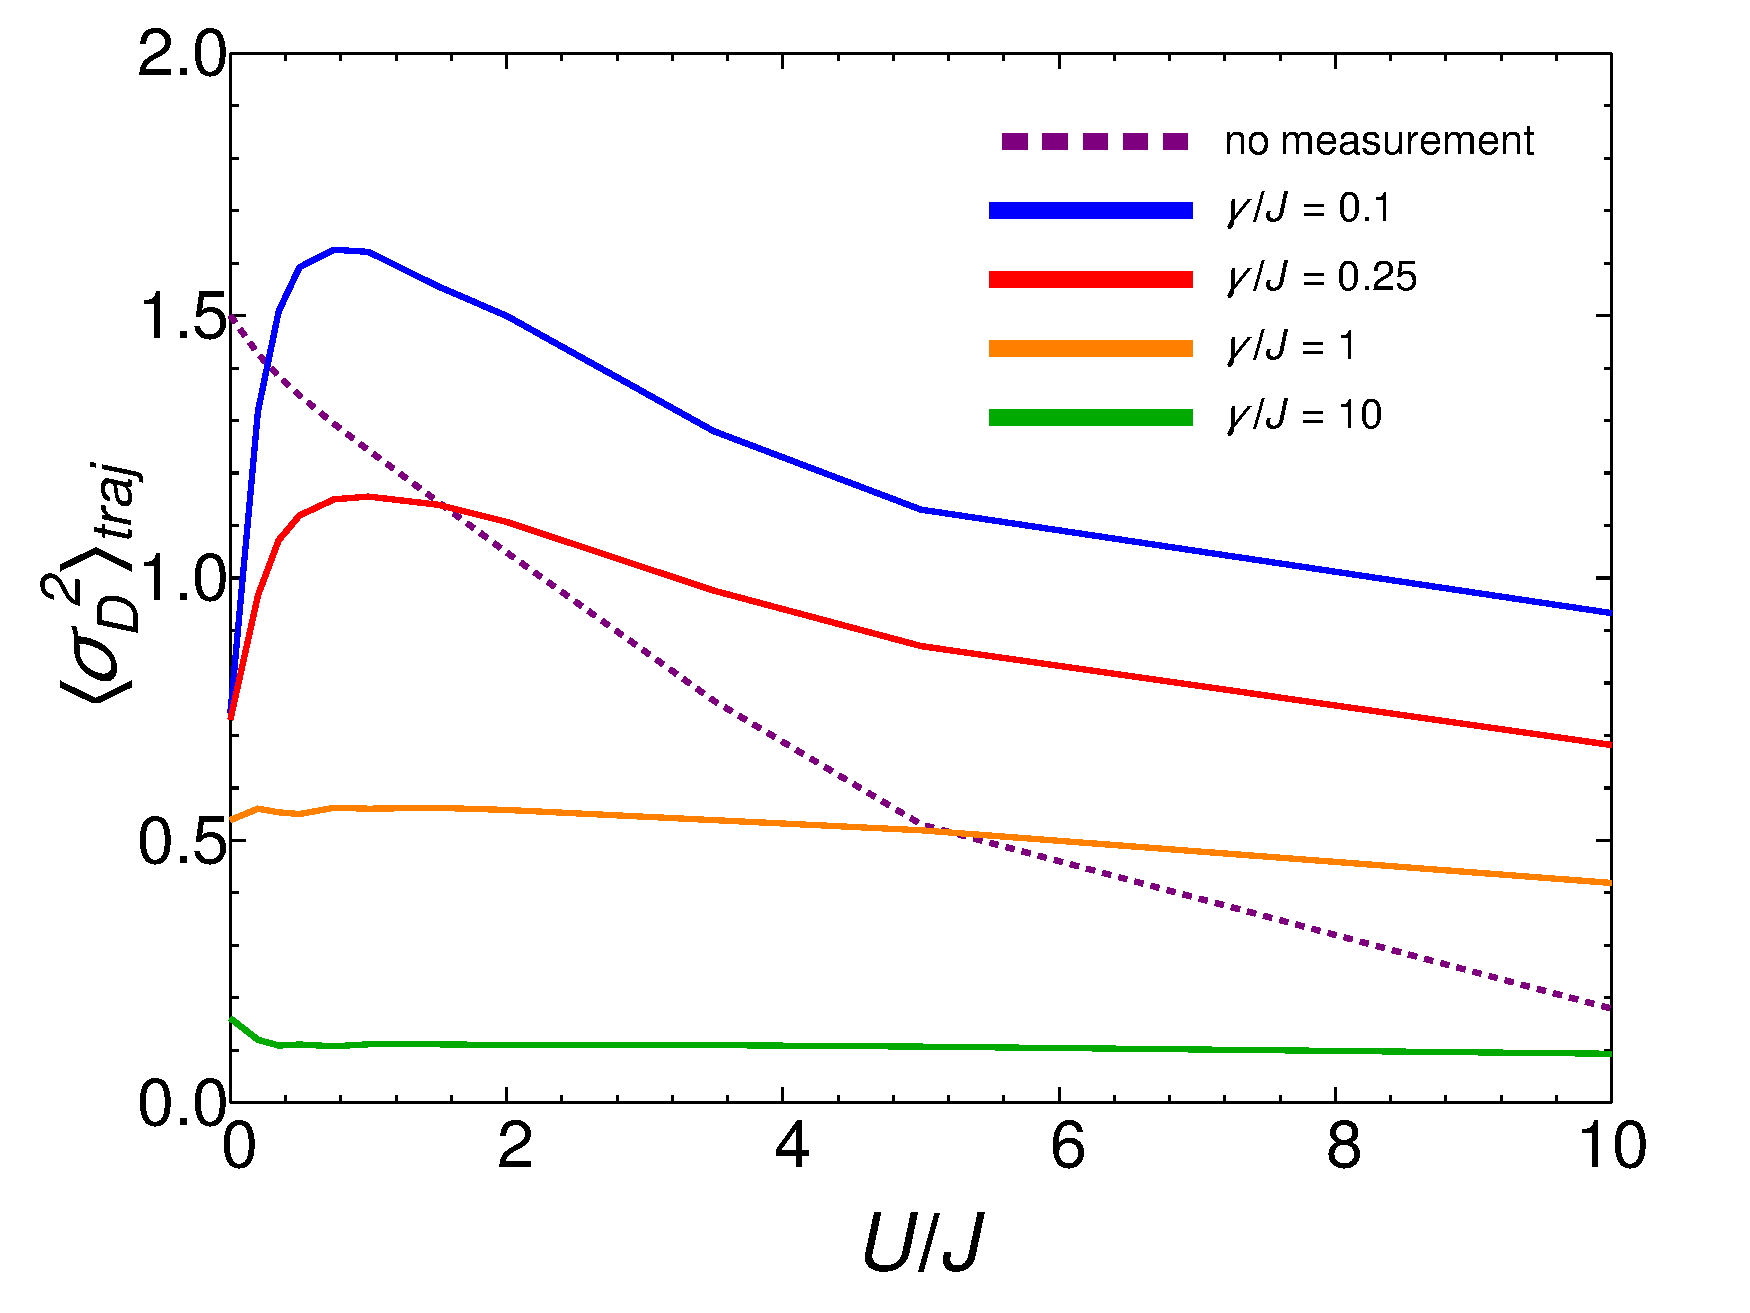
\includegraphics[width=\textwidth]{Squeezing}
  \caption[Squeezing in the presence of Interactions]{Atom number
    fluctuations at odd sites for for $N = 6$ atoms at $M = 6$ sites
    subject to a $\hat{D} = \hat{N}_\mathrm{odd}$ measurement
    demonstrating the competition of global measurement with local
    interactions and tunnelling. Number variances are averaged over
    100 trajectories. Error bars are too small to be shown
    ($\sim 1\%$) which emphasizes the universal nature of the
    squeezing. The initial state used was the ground state for the
    corresponding $U$ and $J$ value. The fluctuations in the ground
    state without measurement decrease as $U / J$ increases,
    reflecting the transition between the supefluid and Mott insulator
    phases. For weak measurement values
    $\langle \sigma^2_D \rangle_\mathrm{traj}$ is squeezed below the
    ground state value for $U = 0$, but it subsequently increases and
    reaches its maximum as the atom repulsion prevents the
    accumulation of atoms prohibiting coherent oscillations thus
    making the squeezing less effective. In the strongly interacting
    limit, the Mott insulator state is destroyed and the fluctuations
    are larger than in the ground state as weak measurement isn't
    strong enough to project into a state with smaller fluctuations
    than the ground state.}
  \label{fig:squeezing}
\end{figure}

First, it is important to note that even though we are dealing with an
average over many trajectories this information cannot be extracted
from a master equation solution. This is because the variance of
$\hat{D}$ as calculated from the density matrix would be dominated by
the uncertainty of the final state. In other words, the fact that the
final value of $\hat{D}$ is undetermined is included in this average
and thus the fluctuations obtained this way are representative of the
variance in the final outcome rather than the squeezing of an
individual conditioned trajectory. This highlights the fact that
interesting physics happens on a single trajectory level which would
be lost if we studied an ensemble average.

\begin{figure}[htbp!]
  \centering
  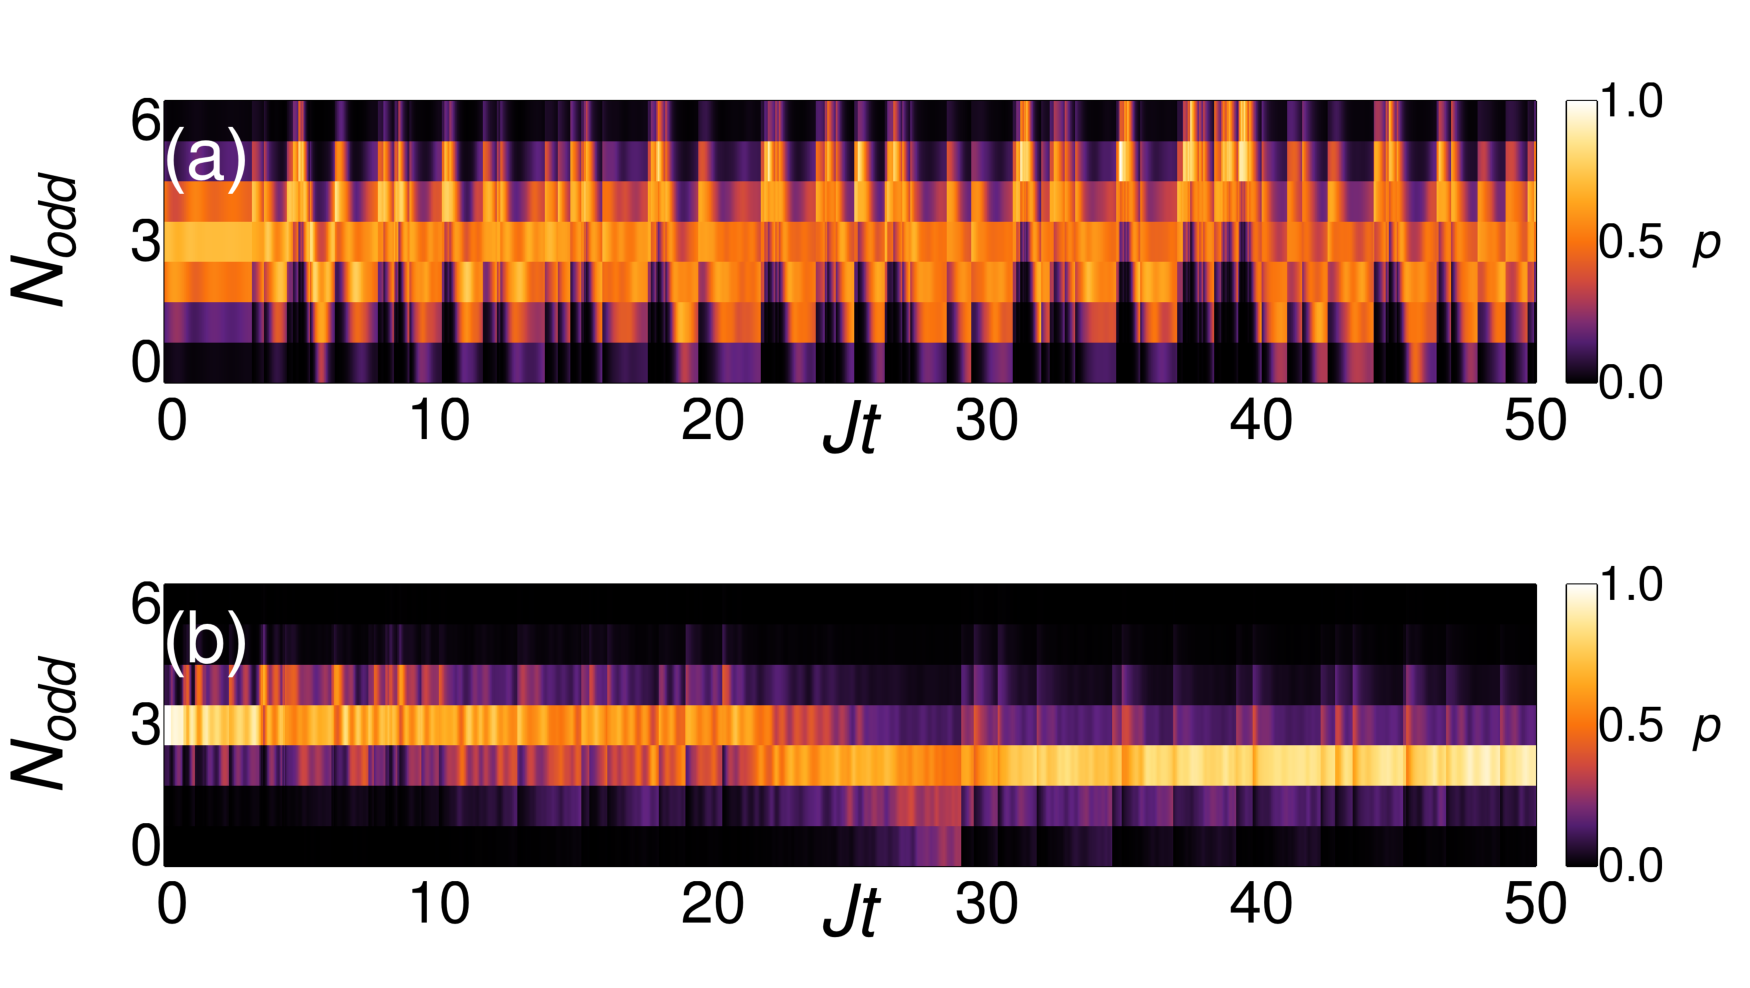
\includegraphics[width=\textwidth]{panel_U}
  \caption[Trajectories in the presence of Interactions]{Conditional
    dynamics of the atom-number distributions at odd sites
    illustrating competition of the global measurement with local
    interactions and tunnelling. The plots are for single quantum
    trajectores starting from the ground state for $N = 6$ atoms on
    $M = 6$ sites with $\hat{D} = \hat{N}_\mathrm{odd}$,
    $\gamma/J = 0.1$. (a) Weakly interacting bosons $U/J = 1$: the
    on-site repulsion prevents the formation of well-defined
    oscillation in the population of the mode. As states with
    different imbalance evolve with different frequencies, the
    squeezing is not as efficient for the non-interacting case. (b)
    Strongly interacting bosons $U/J = 10$: oscillations are
    completely supressed and the number of atoms in the mode is rather
    well-defined although clearly worse than in a Mott insulator.}
  \label{fig:Utraj}
\end{figure}

Looking at Fig. \ref{fig:squeezing} we see many interesting things
happening suggesting different regimes of behaviour. For the ground
state (i.e.~no measurement) we see that the fluctuations decrease
monotonically as $U$ increases reflecting the superfluid to Mott
insulator quantum phase transition. The measured state on the other
hand behaves very differently and
$\langle \sigma^2_D \rangle_\mathrm{traj}$ varies
non-monotonically. For weak interactions the fluctuations are strongly
squeezed below those of the ground state followed by a rapid increase
as $U$ is increased before peaking and eventually decreasing. We have
already seen in the previous section and in particular
Fig. \ref{fig:oscillations} that the macroscopic oscillations at
$U = 0$ are well squeezed when compared to the inital state and this
is the case over here as well. However, as $U$ is increased the
interactions prevent the atoms from accumulating in one place thus
preventing oscillations with a large amplitude which effectively makes
the squeezing less effective as seen in Fig. \ref{fig:Utraj}a. In
fact, we have seen towards the end of the last section how for small
amplitude oscillations that can be described by the effective
double-well model the width of the number distribution does not change
by much. Even though that model is not valid for $U \ne 0$ we should
not be surprised that without macroscopic oscillations the
fluctuations cannot be significantly reduced.

On the other end of the spectrum, for weak measurement, but strong
on-site interactions we note that the backaction leads to a
significant increase in fluctuations compared to the ground
state. This is simply due to the fact that the measurement destroys
the Mott insulating state, which has small fluctuations due to strong
local interactions, but then subsequently is not strong enough to
squeeze the resulting dynamics as shown in Fig. \ref{fig:Utraj}b. To
see why this is so easy for the quantum jumps to do we look at the
ground state in first-order perturbation theory given by
\begin{equation}
  | \Psi_{J/U} \rangle = \left[ 1 + \frac{J}{U} \sum_{\langle i, j
      \rangle} \bd_i b_j \right] | \Psi_0 \rangle,
\end{equation}
where we have neglected the non-Hermitian term as we're in the weak
measurement regime and $| \Psi_0 \rangle$ is the Mott insulator state and the second
term in the brackets represents a uniform distribution of
particle-hole excitation pairs across the lattice. In the
$U \rightarrow \infty$ limit a quantum jump has no effect as
$| \Psi_0 \rangle$ is already an eigenstate of $\hat{D}$. However, for
finite $U$, each photocount will amplify the present excitations
increasing the fluctuations in the system. In fact, consecutive
detections lead to an exponential growth of these excitations. For
$K \gg 1$ illuminated sites and unit filling of the lattice, the
atomic state after $m$ consecutive quantum jumps becomes
$\c^m | \Psi_{J/U} \rangle \propto | \Psi_{J/U} \rangle + | \Phi_m
\rangle$ where
\begin{equation}
  | \Phi_m \rangle = \frac{2^m J} {K U} \sum_{i \in
    \mathrm{odd}} \left( \bd_i b_{i-1} - \bd_{i-1} b_i - \bd_{i+1} b_i
    + \bd_i b_{i+1} \right) | \Psi_0 \rangle.
\end{equation}
In the weak measurement regime the effect of non-Hermitian decay is
negligible compared to the local atomic dynamics combined with the
quantum jumps so there is minimal dissipation occuring. Therefore,
because of the exponential growth of the excitations, even a small
number of photons arriving in succession can destroy the ground
state. We have neglected all dynamics in between the jumps which would
distribute the new excitations in a way which will affect and possibly
reduce the effects of the subsequent quantum jumps. However, due to
the lack of any decay channels they will remain in the system and
subsequent jumps will still amplify them further destroying the ground
state and thus quickly leading to a state with large fluctuations.

In the strong measurement regime ($\gamma \gg J$) the measurement
becomes more significant than the local dynamics and the system will
freeze the state in the measurement operator eigenstates. In this
case, the squeezing will always be better than in the ground state,
because measurement and on-site interaction cooperate in suppressing
fluctuations. This cooperation did not exist for weak measurement,
because it tried to induce dynamics which produced squeezed states
(either succesfully as seen with the macroscopic oscillations or
unsuccesfully as seen with the Mott insulator). This suffered heavily
from the effects of interactions as they would prevent this dynamics
by dephasing different components of the coherent excitations. Strong
measurement, on the other hand, squeezes the quantum state by trying
to project it onto an eigenstate of the observable
\cite{mekhov2009prl, mekhov2009prl}. For weak interactions where the
ground state is a highly delocalised superfluid it is obvious that
projections onto $\hat{D} = \hat{N}_\mathrm{odd}$ will supress
fluctuations significantly. However, the strongly interacting regime
is much less evident, especially since we have just demonstrated how
sensitive the Mott insulating phase is to the quantum jumps when the
measurement is weak.

To understand the strongly interacting case we will again use
first-order perturbation theory and consider a postselected
$\langle \hat{D}^\dagger \hat{D} \rangle = 0$ trajectory. This
corresponds to a state that scatters no photons and thus is fully
described by the non-Hermitian Hamiltonian alone. Squeezing depends on
the measurement and interaction strengths and is common to all the
possible trajectories so we can gain insight into the general
behaviour by considering a specific special case. However, we will
instead consider
$\hat{D} = \Delta \hat{N} = \hat{N}_\mathrm{odd} -
\hat{N}_\mathrm{even}$, because this measurement also has only $Z = 2$
modes, but its $\langle \hat{D}^\dagger \hat{D} \rangle = 0$
trajectory would be very close to the Mott insulating ground state,
because $\hat{D}^\dagger \hat{D} | \Psi_0 \rangle = 0$ and we can
expand around the Mott insulating state. Applying perturbation theory
to obtain the modified ground state we get
\begin{equation}
  | \Psi_{J,U, \gamma} \rangle = \left[ 1 + \frac{J}{U - i 4 \gamma} \sum_{\langle i, j
      \rangle} \bd_i b_j \right] | \Psi_0 \rangle.
\end{equation}
The variance of the measurement operator for this state is given by
\begin{equation}
  \sigma^2_{\Delta N} = \frac{16 J^2 M} {U^2 + 16 \gamma^2}.
\end{equation}
From the form of the denominator we immediately see that both
interaction and measurement squeeze with the same quadratic dependence
and that the squeezing is always better than in the ground state
($\gamma = 0$) regardless of the value of $U$. Also, depending on the
ratio of $\gamma/U$ the squeezing can be dominated by measurement
($\gamma/U \gg 1$) or by interactions ($\gamma/U \ll 1$) or both
processes can contribute equally ($\gamma/U \approx 1$). The
$\hat{D} = \hat{N}_\mathrm{odd}$ measurement will behave similarly
since the geometry is exactly the same. Furthermore, the Mott
insulator state is also an eigenstate of this operator, just not the
zero eigenvalue vector and thus the final state would need to be
described using a balance of quantum jumps and non-Hermitian evolution
complicating the picture. However, the particle-hole excitation term
would be proportional to $(U^2 + \gamma^2)^{-1}$ instead since the
$\gamma$ coefficient in the perturbative expansion depends on
$(J_{i,i} - J_{i\pm1,i\pm1})^2$. We can see the system transitioning
into the strong measurement regime in Fig. \ref{fig:squeezing} as the
$U$-dependence flattens out with increasing measurement strength as
the $\gamma/U \gg 1$ regime is reached.

\subsection{Emergent Long-Range Correlated Tunnelling}

When $\gamma \rightarrow \infty$ the measurement becomes
projective. This means that as soon as the probing begins, the system
collapses into one of the observable's eigenstates. Furthermore, since
this measurement is continuous and doesn't stop after the projection
the system will be frozen in this state. This effect is called the
quantum Zeno effect \cite{misra1977, facchi2008} from Zeno's classical
paradox in which a ``watched arrow never moves'' that stated that
since an arrow in flight is not seen to move during any single
instant, it cannot possibly be moving at all. Classically the paradox
was resolved with a better understanding of infinity and infintesimal
changes, but in the quantum world a watched quantum arrow will in fact
never move. The system is being continuously projected into its
initial state before it has any chance to evolve. If degenerate
eigenspaces exist then we can observe quantum Zeno dynamics where
unitary evolution is uninhibited within such a degenerate subspace,
called the Zeno subspace \cite{facchi2008, raimond2010, raimond2012,
  signoles2014}.

These effects can be easily seen in our model when
$\gamma \rightarrow \infty$. The system will be projected into one or
more degenerate eignstates of $\cd \c$, $| \psi_i \rangle$, for which
we define the projector
$P_\varphi = \sum_{i \in \varphi} | \psi_i \rangle$ where $\varphi$
denotes a single degenerate subspace. The Zeno subspace is determined
randomly as per the Copenhagen postulates and thus it depends on the
initial state. If the projection is into the subspace $\varphi$, the
subsequent evolution is described by the projected Hamiltonian
$P_{\varphi} \hat{H}_0 P_{\varphi}$. We have used the original
Hamiltonian, $\hat{H}_0$, without the non-Hermitian term or the
quantum jumps as their combined effect is now described by the
projectors. Physically, in our model of ultracold bosons trapped in a
lattice this means that tunnelling between different spatial modes is
completely supressed since this process couples eigenstates belonging
to different Zeno subspaces. If a small connected part of the lattice
was illuminated uniformly such that $\hat{D} = \hat{N}_K$ then
tunnelling would only be prohibited between the illuminated and
unilluminated areas, but dynamics proceeds normally within each zone
separately. However, the goemetric patterns we have in which the modes
are spatially delocalised in such a way that neighbouring sites never
belong to the same mode, e.g.  $\hat{D} = \hat{N}_\mathrm{odd}$, would
lead to a complete suppression of tunnelling across the whole lattice
as there is no way for an atom to tunnel within this Zeno subspace
without first having to leave it.

This is an interesting example of the quantum Zeno effect and dynamics
and it can be used to prohibit parts of the dynamics of the
Bose-Hubbard Model in order to engineer desired Hamiltonians for
quantum simulations or other applications. However, the infinite
projective limit is uninteresting in the context of a global
measurement scheme. The same effects and Hamiltonians can be achieved
using multiple independent measurements which address a few sites
each. In order to take advantage of the nonlocal nature of the
measurement it turns out that we need to consider a finite limit for
$\gamma \gg J$. By considering a non-infinite $\gamma$ we observe
additional dynamics while the usual atomic tunnelling is still heavily
Zeno-suppressed. These new effects are shown in Fig. \ref{fig:zeno}.

\begin{figure}[hbtp!]
  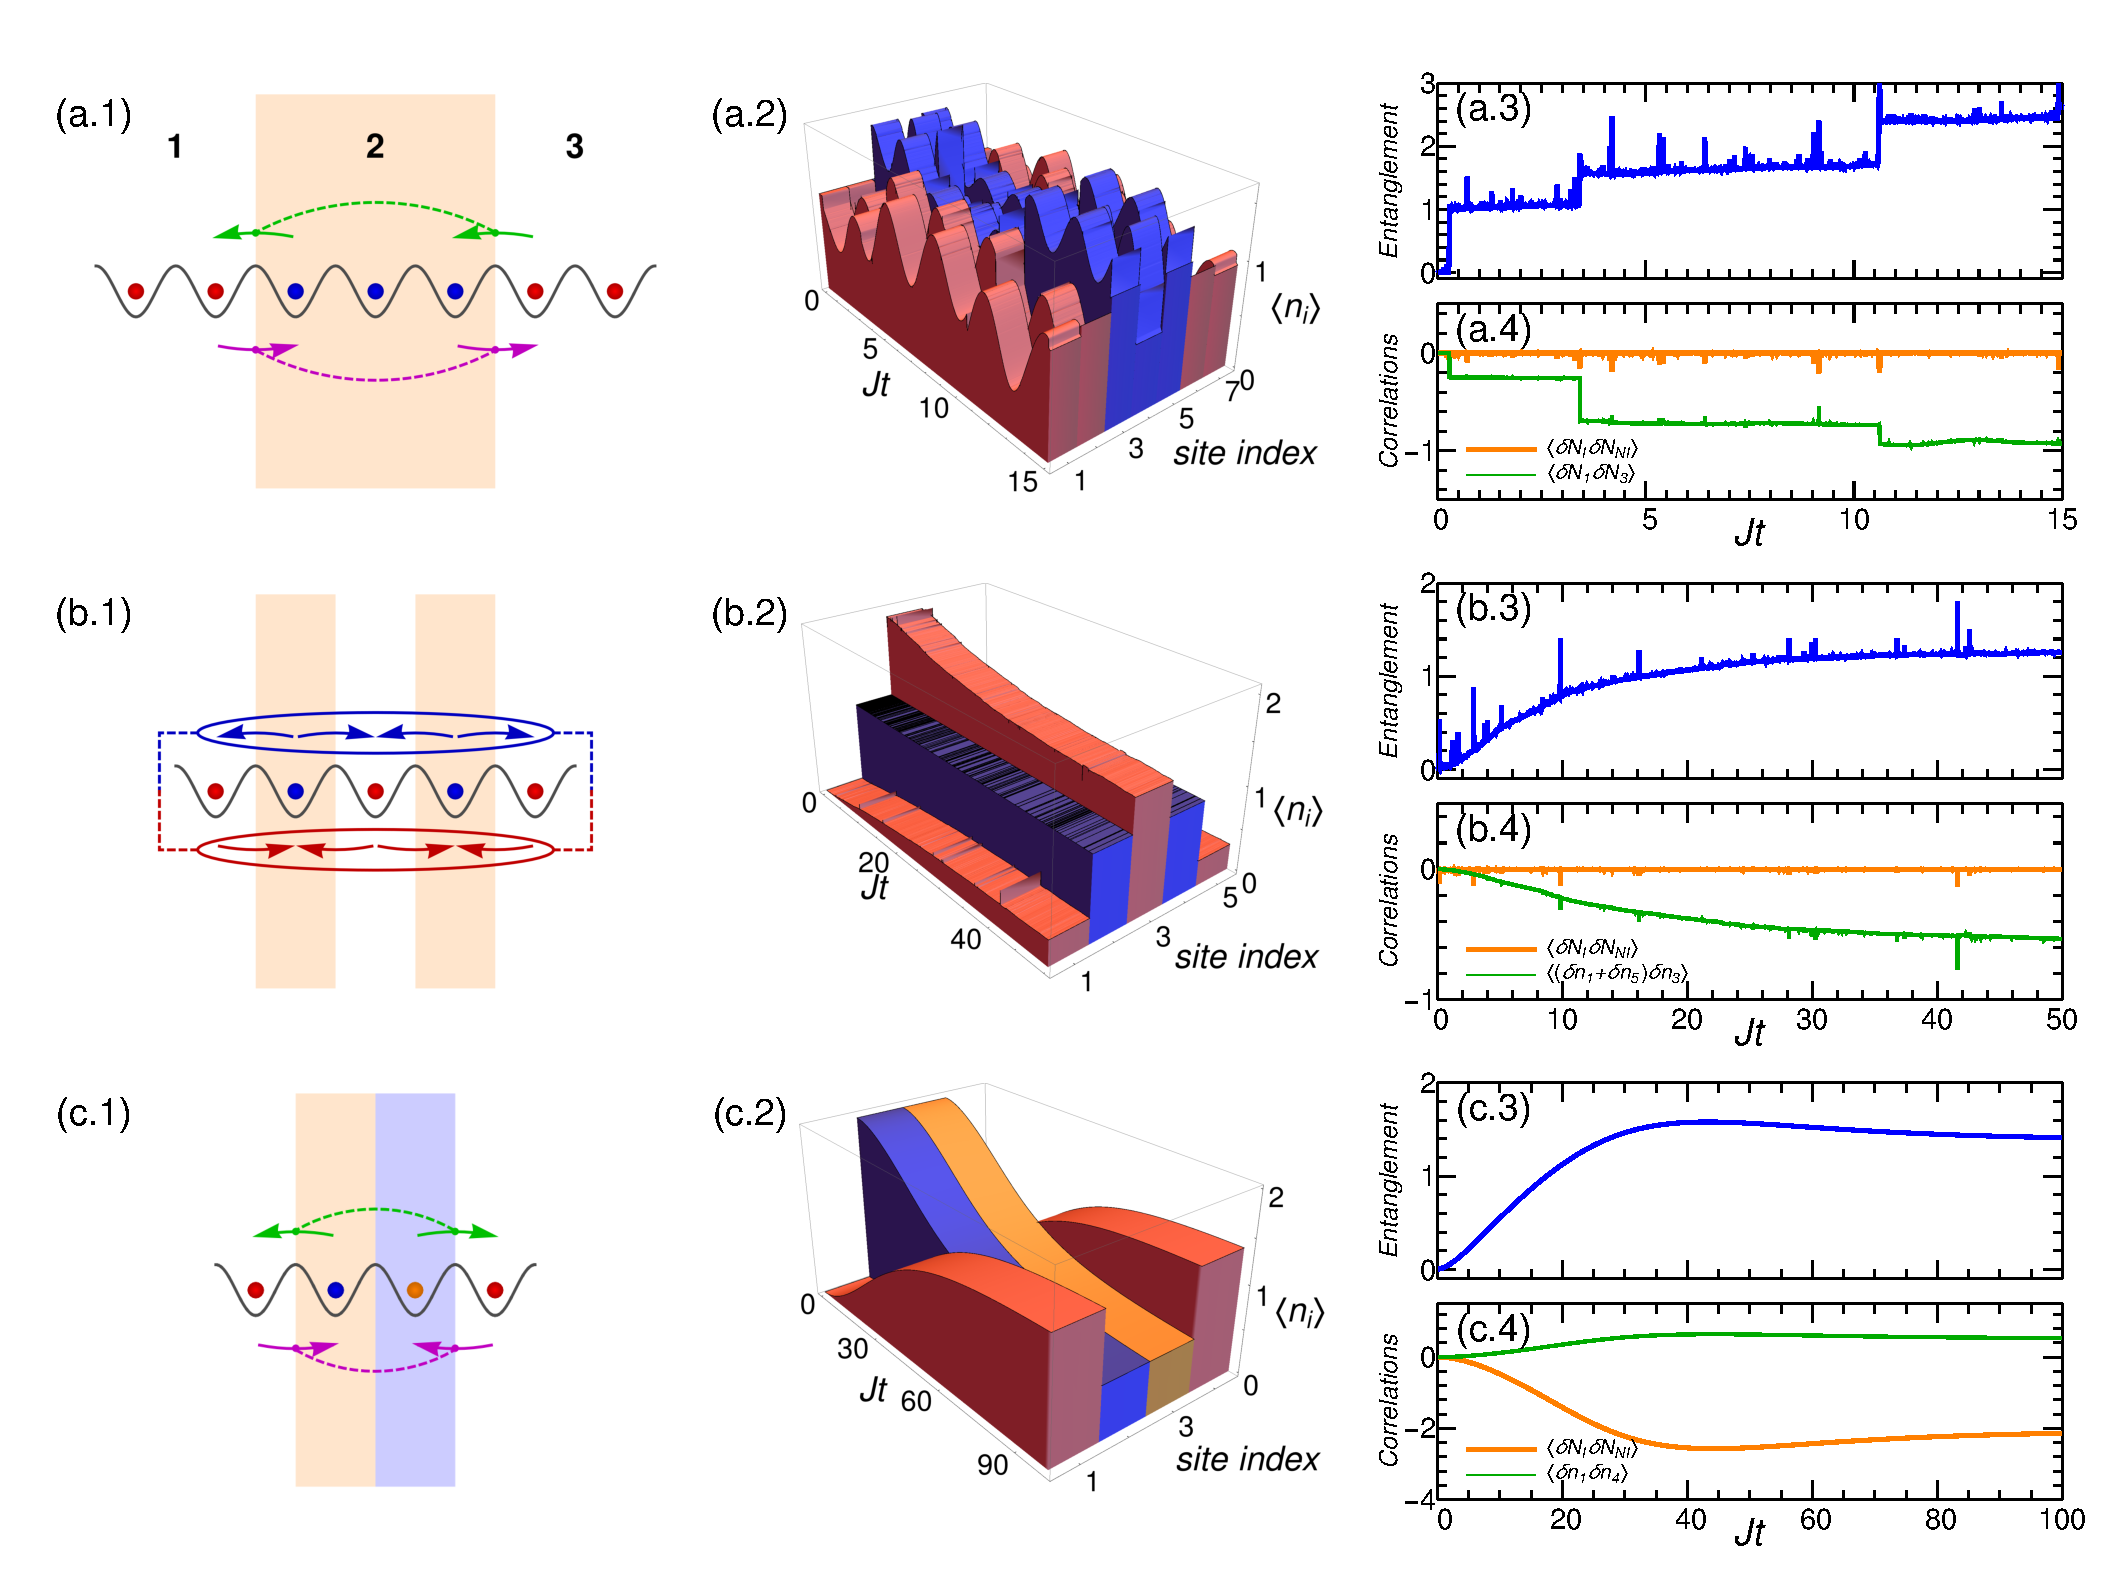
\includegraphics[width=\textwidth]{Zeno.pdf}
  \caption[Emergent Long-Range Correlated Tunnelling]{ Long-range
    correlated tunneling and entanglement, dynamically induced by
    strong global measurement in a single quantum
    trajectory. (a),(b),(c) show different measurement geometries,
    implying different constraints. Panels (1): schematic
    representation of the long-range tunneling processes. Panels (2):
    evolution of on-site densities. Panels (3): entanglement entropy
    growth between illuminated and non-illuminated regions. Panels
    (4): correlations between different modes (orange) and within the
    same mode (green); $N_I$ ($N_{NI}$) is the atom number in the
    illuminated (non-illuminated) mode.  (a) (a.1) Atom number in the
    central region is frozen: system is divided into three
    regions. (a.2) Standard dynamics happens within each region, but
    not between them. (a.3) Entanglement build up. (a.4) Negative
    correlations between non-illuminated regions (green) and zero
    correlations between the $N_I$ and $N_{NI}$ modes
    (orange). Initial state: $|1,1,1,1,1,1,1 \rangle$, $\gamma/J=100$,
    $J_{jj}=[0,0,1,1,1,0,0]$.  (b) (b.1) Even sites are illuminated,
    freezing $N_\text{even}$ and $N_\text{odd}$. Long-range tunneling
    is represented by any pair of one blue and one red arrow. (b.2)
    Correlated tunneling occurs between non-neighbouring sites without
    changing mode populations. (b.3) Entanglement build up. (b.4)
    Negative correlations between edge sites (green) and zero
    correlations between the modes defined by $N_\text{even}$ and
    $N_\text{odd}$ (orange). Initial state: $|0,1,2,1,0 \rangle$,
    $\gamma/J=100$, $J_{jj}=[0,1,0,1,0]$.  (c) (c.1,2) Atom number
    difference between two central sites is frozen. (c.3) Entanglement
    build up. (c.4) In contrast to previous examples, sites in the
    same zones are positively correlated (green), while atoms in
    different zones are negatively correlated (orange). Initial state:
    $|0,2,2,0 \rangle$, $\gamma/J=100$, $J_{jj}=[0,-1,1,0]$. 1D
    lattice, $U/J=0$.}
  \label{fig:zeno}
\end{figure}

There are two crucial features of the resulting dynamics that are of
note. First, just like in the infinite quantum Zeno limit the
evolution between nearest neighbours within the same mode is
unperturbed whilst tunnelling between different modes is heavily
suppressed by the measurement. Therefore, we see the usual quantum
Zeno dynamics within a single Zeno subspace and just like before, it
is also possible to use the global probing scheme to engineer these
eigenspaces and select which tunnelling processes should be
uninhibited and which should be suppressed. However, there is a second
effect that was not present before. In Fig. \ref{fig:zeno} we can
observe tunnelling that violates the boundaries established by the
spatial modes. When $\gamma$ is finite, second-order processes,
i.e.~two correlated tunnelling events, can now occur via an
intermediate (virtual) state outside of the Zeno subspace as long as
the Zeno subspace of the final state remains the same. Crucially,
these tunnelling events are only correlated in time, but not in
space. This means that the two events do not have to occur for the
same atom or even at the same site in the lattice. As long as the Zeno
subspace is preserved, these processes can occur anywhere in the
system. That is, a pair of atoms separated by many sites is able to
tunnel in a correlated manner. This is only possible due to the
ability of creating extensive and spatially nonlocal modes as
described in section \ref{sec:modes} which in turn is enabled by the
global nature of the measurement. This would not be possible to
achieve with local measurements as the Zeno subspaces would be
described entirely by local variables which cannot be preserved by
such delocalised tunnelling events.

In the subsequent sections we will rigorously derive the following
Hamiltonian for the non-interacting dynamics within a single Zeno
subspace, $\varphi = 0$, for a lattice where the measurement defines
$Z = 2$ distinct modes, e.g. $\hat{D} = \hat{N}_K$ or
$\hat{D} = \hat{N}_\mathrm{odd}$
\begin{equation}
  \label{eq:hz}
  \hat{H}_\varphi = P_0 \left[ -J \sum_{\langle i, j \rangle}
    b^\dagger_i b_j - i \frac{J^2} {A \gamma} \sum_{\varphi} 
    \sum_{\substack{\langle i \in \varphi, j \in \varphi^\prime
        \rangle \\ \langle k \in \varphi^\prime, l \in \varphi
        \rangle}} b^\dagger_i b_j b^\dagger_k b_l \right] P_0,
\end{equation}
where
$A = (J_{\varphi,\varphi} - J_{\varphi^\prime,\varphi^\prime})^2$ is a
constant that depends on the measurement scheme, $\varphi$ denotes a
set of sites belonging to a single mode and $\varphi^\prime$ is the
set's complement (e.g.~odd and even or illuminated and non-illuminated
sites). We see that this Hamiltonian consists of two parts. The first
term corresponds to the standard quantum Zeno first-order dynamics
that occurs within a Zeno subspace, i.e.~tunnelling between
neighbouring sites that belong to the same mode. Otherwise, if $i$ and
$j$ belong to different modes $P_0 \bd_i b_j P_0 = 0$. When
$\gamma \rightarrow \infty$ we recover the quantum Zeno Hamiltonian
where this would be the only remaining term. It is the second term
that shows the second-order corelated tunnelling terms. This is
evident from the inner sum which requires that pairs of sites ($i$,
$j$) and ($k$, $l$) between which atoms tunnel must be nearest
neighbours, but these pairs can be anywhere on the lattice within the
constraints of the mode structure. This is in particular explicitly
shown in Figs. \ref{fig:zeno}(a,b). The imaginary coefficient means
that the tinelling behaves like an exponential decay (overdamped
oscillations). This also implies that the norm will decay, but this
does not mean that there are physical losses in the system. Instead,
the norm itself represents the probability of the system remaining in
the $\varphi = 0$ Zeno subspace. Since $\gamma$ is not infinite there
is now a finite probability that the stochastic nature of the
measurement will lead to a discontinous change in the system where the
Zeno subspace rapidly changes which can be seen in
Fig. \ref{fig:zeno}(a). However, later in this chapter we will see
that steady states of this Hamiltonian exist which will no longer
change Zeno subspaces.

Crucially, what sets this effect apart from usual many-body dynamics
with short-range interactions is that first order processes are
selectively suppressed by the global conservation of the measured
observable and not by the prohibitive energy costs of doubly-occupied
sites, as is the case in the $t$-$J$ model \cite{auerbach}. This has
profound consequences as this is the physical origin of the long-range
correlated tunneling events represented in Eq. \eqref{eq:hz} by the
fact that the pairs ($i$, $j$) and ($k$, $l$) can be very distant. The
projection $\hat{P}_0$ is not sensitive to individual site
occupancies, but instead enforces a fixed value of the observable,
i.e.~a single Zeno subspace. This is a striking difference with the
$t$-$J$ and other strongly interacting models. The strong interaction
also leads to correlated events in which atoms can tunnel over each
other by creating an unstable doubly occupied site during the
intermediate step. However, these correlated events are by their
nature localised. Due to interactions the doubly-occupied site cannot
be present in the final state which means that any tunnelling event
that created this unstable configuration must be followed by another
tunnelling event which takes an atom away. In the case of global
measurement this process is delocalised, because since the modes
consist of many sites the stable configuration can be restored by a
tunnelling event from a completely different lattice site that belongs
to the same mode.

In Fig.~\ref{fig:zeno}a we consider illuminating only the central
region of the optical lattice and detecting light in the diffraction
maximum, thus we freeze the atom number in the $K$ illuminated sites
$\hat{N}_\text{K}$~\cite{mekhov2009prl,mekhov2009pra}. The measurement
scheme defines two different spatial modes: the non-illuminated zones
$1$ and $3$ and the illuminated one $2$. Figure~\ref{fig:zeno}(a.2)
illustrates the evolution of the mean density at each lattice site:
typical dynamics occurs within each region but the standard tunnelling
between different modes is suppressed. Importantly, second-order
processes that do not change $N_\text{K}$ are still possible since an
atom from $1$ can tunnel to $2$, if simultaneously one atom tunnels
from $2$ to $3$. Therefore, effective long-range tunneling between two
spatially disconnected zones $1$ and $3$ happens due to the two-step
processes $1 \rightarrow 2 \rightarrow 3$ or
$3 \rightarrow 2 \rightarrow 1$. These transitions are responsible for
the negative (anti-)correlations
$\langle \delta N_1 \delta N_3 \rangle = \langle N_1 N_3 \rangle -
\langle N_1 \rangle \langle N_3 \rangle$ showing that an atom
disappearing from zone $1$ appears in zone $3$, while there are no
number correlations between illuminated and non-illuminated regions,
$\langle( \delta N_1 + \delta N_3 ) \delta N_2 \rangle = 0$ as shown
in Fig.~\ref{fig:zeno}(a.4). In contrast to fully-projective
measurement, the existence of an intermediate (virtual) step in the
correlated tunnelling process builds long-range entanglement between
illuminated and non-illuminated regions as shown in
Fig.~\ref{fig:zeno}(a.3).

To make correlated tunneling visible even in the mean atom number, we
suppress the standard Bose-Hubbard dynamics by illuminating only the
even sites of the lattice in Fig.~\ref{fig:zeno}(b). Even though this
measurement scheme freezes both $N_\text{even}$ and $N_\text{odd}$,
atoms can slowly tunnel between the odd sites of the lattice, despite
them being spatially disconnected. This atom exchange spreads
correlations between non-neighbouring lattice sites on a time scale
$\sim \gamma/J^2$ as seen in Eq. \eqref{eq:hz}. The schematic
explanation of long-range correlated tunneling is presented in
Fig.~\ref{fig:zeno}(b.1): the atoms can tunnel only in pairs to assure
the globally conserved values of $N_\text{even}$ and $N_\text{odd}$,
such that one correlated tunneling event is represented by a pair of
one red and one blue arrow. Importantly, this scheme is fully
applicable for a lattice with large atom and site numbers, well beyond
the numerical example in Fig.~\ref{fig:zeno}(b.1), because as we can
see in Eq. \eqref{eq:hz} it is the geometry of quantum measurement that
assures this mode structure (in this example, two modes at odd and
even sites) and thus the underlying pairwise global tunnelling.

The scheme in Fig.~\ref{fig:zeno}(b.1) can help design a nonlocal
reservoir for the tunneling (or ``decay'') of atoms from one region to
another. For example, if the atoms are placed only at odd sites,
according to Eq. \eqref{eq:hz} their tunnelling is suppressed since the
multi-tunneling event must be successive, i.e.~an atom tunnelling into
a different mode, $\varphi^\prime$, must then also tunnel back into
its original mode, $\varphi$. If, however, one adds some atoms to even
sites (even if they are far from the initial atoms), the correlated
tunneling events become allowed and their rate can be tuned by the
number of added atoms. This resembles the repulsively bound pairs
created by local interactions \cite{winkler2006, folling2007}. In
contrast, here the atom pairs are nonlocally correlated due to the
global measurement. Additionally, these long-range correlations are a
consequence of the dynamics being constrained to a Zeno subspace: the
virtual processes allowed by the measurement entangle the spatial
modes nonlocally. Since the measurement only reveals the total number
of atoms in the illuminated sites, but not their exact distribution,
these multi-tunelling events cause the build-up of long range
entanglement. This is in striking contrast to the entanglement caused
by local processes which can be very confined, especially in 1D where
it is typically short range. This makes numerical calculations of our
system for large atom numbers really difficult, since well-known
methods such as DMRG and MPS \cite{schollwock2005} (which are
successful for short-range interactions) rely on the limited extent of
entanglement.

The negative number correlations are typical for systems with
constraints (superselection rules) such as fixed atom number. The
effective dynamics due to our global, but spatially structured,
measurement introduces more general constraints to the evolution of
the system. For example, in Fig.~\ref{fig:zeno}(c) we show the
generation of positive number correlations shown in
Fig.~\ref{fig:zeno}(c.4) by freezing the atom number difference
between the sites ($N_\text{odd}-N_\text{even}$). Thus, atoms can only
enter or leave this region in pairs, which again is possible due to
correlated tunneling as seen in Figs.~\ref{fig:zeno}(c.1,c.2) and
manifests positive correlations. As in the previous example, two edge
modes in Fig.~\ref{fig:zeno}(c) can be considered as a nonlocal
reservoir for two central sites, where a constraint is applied. Note
that, using more modes, the design of higher-order multi-tunneling
events is possible.

This global pair tunneling may play a role of a building block for
more complicated many-body effects. For example, a pair tunneling
between the neighbouring sites has been recently shown to play
important role in the formation of new quantum phases, e.g., pair
superfluid \cite{sowinski2012} and lead to formulation of extended
Bose-Hubbard models \cite{omjyoti2015}. The search for novel
mechanisms providing long-range interactions is crucial in many-body
physics. One of the standard candidates is the dipole-dipole
interaction in, e.g., dipolar molecules, where the mentioned pair
tunneling between even neighboring sites is already considered to be
long-range \cite{sowinski2012,omjyoti2015}. In this context, our work
suggests a fundamentally different mechanism originating from quantum
optics: the backaction of global and spatially structured measurement,
which as we prove can successfully compete with other short-range
processes in many-body systems. This opens promising opportunities for
future research.

\section{Non-Hermitian Dynamics in the Quantum Zeno Limit}

In the previous section we provided a rather high-level analysis of
the strong measurement limit in our quantum gas model. We showed that
global measurement in the strong, but not projective, limit leads to
correlated tunnelling events which can be highly delocalised. Multiple
examples for different optical geometries and measurement operators
demonstrated the incredible felixbility and potential in engineering
dynamics for ultracold gases in an optical lattice. We also claimed
that the behaviour of the system is described by the Hamiltonian given
in Eq. \eqref{eq:hz}. Having developed a physical and intuitive
understanding of the dynamics in the quantum Zeno limit we will now
provide a more rigorous, low-level and fundamental understanding of
the process.

\subsection{Suppression of Coherences in the Density Matrix}

At this point we deviate from the quantum trajectory approach and we
resort to a master equation as introduced in section
\ref{sec:master}. We do this, because we have seen that the emergent
long-range correlated tunnelling is a feature of all trajectories and
mostly depends on the geometry of the measurement. Therefore, a
general approach starting from an unconditioned state should be able
to reveal these features. However, we will later make use of the fact
that we are in possession of a measurement record and obtain a
conditioned state. Furthermore, we first consider the most general
case of an open system subject to a quantum measurement and only limit
ourselves to the quantum gas model later on. This demonstrates that
the dynamics we observed in the previous section are a feature of
measurement rather than our specific model.

As introduced in section \ref{sec:master} we consider a state
described by the density matrix $\hat{\rho}$ whose isolated behaviour
is described by the Hamiltonian $\H_0$ and when measured the jump
operator $\c$ is applied to the state at each detection
\cite{MeasurementControl}. The master equation describing its time
evolution when we ignore the measurement outcomes is given by
\begin{equation}
  \dot{\hat{\rho}} = -i [ \H_0 , \hat{\rho} ] + \c \hat{\rho} \cd - \frac{1}{2}(
  \cd\c \hat{\rho} + \hat{\rho} \cd\c ).
\end{equation}
We also define $\c = \lambda \op$ and $\H_0 = \nu \h$. The exact
definition of $\lambda$ and $\nu$ is not so important as long as these
coefficients can be considered to be some measure of the relative size
of these operators. They would have to be determined on a case-by-case
basis, because the operators $\c$ and $\H_0$ may be unbounded. If
these operators are bounded, one can simply define them such that
$||\op|| \sim O(1)$ and $||\h|| \sim O(1)$. If they are unbounded, one
possible approach would be to identify the relevant subspace of which
dynamics we are interested in and scale the operators such that the
eigenvalues of $\op$ and $\h$ in this subspace are $\sim O(1)$.

We will once again use projectors $P_m$ which have no effect on states
within a degenerate subspace of $\c$ ($\op$) with eigenvalue $c_m$
($o_m$), but annihilate everything else. For convenience we will also
use the following definition $\hat{\rho}_{mn} = P_m \hat{\rho} P_n$.
Note that these are submatrices of the density matrix, which in
general are not single matrix elements. Therefore, we can write the
master equation that describes this open system as a set of equations
\begin{equation}
\label{eq:master}
  \dot{\hat{\rho}}_{mn} =  -i K P_m \left[ \h \sum_r \hat{\rho}_{rn}
    - \sum_r \hat{\rho}_{mr} \h \right] P_n + \lambda^2 \left[ o_m
    o_n^*  - \frac{1}{2} \left( |o_m|^2 + |o_n|^2 \right) \right] \hat{\rho}_{mn},
\end{equation}
where the first term describes coherent evolution whereas the second
term causes dissipation. 

First, note that for the density submatrices for which $m = n$,
$\hat{\rho}_{mm}$, the dissipative term vanishes. This means that
these submatrices are subject to coherent evolution only and do not
experience losses and they are thus decoherence free subspaces. It is
crucial to note that these submatrices are simply the density matrices
of the individual degenerate Zeno subspaces. Interestingly, any state
that consists only of these decoherence free subspaces, i.e.~
$\hat{\rho} = \sum_m \hat{\rho}_{mm}$, and that commutes with the
Hamiltonian, $[\hat{\rho}, \hat{H}_0] = 0$, will be a steady state.
This can be seen by substituting this ansatz into
Eq. \eqref{eq:master} which yields $\dot{\hat{\rho}}_{mn} = 0$ for all
$m$ and $n$. These states can be prepared dissipatively using known
techniques \cite{diehl2008}, but it is not required that the state be
a dark state of the dissipative operator as is usually the case.

Second, we consider a large detection rate, $\lambda^2 \gg \nu$, for
which the coherences, i.e.~ the density submatrices $\hat{\rho}_{mn}$
for which $m \ne n$, will be heavily suppressed by dissipation. We can
adiabatically eliminate these cross-terms by setting
$\dot{\hat{\rho}}_{mn} = 0$, to get
\begin{equation}
\label{eq:intermediate}
\hat{\rho}_{mn} = \frac{\nu}{\lambda^2} \frac{i P_m \left[ \h \sum_r \hat{\rho}_{rn} - \sum_r \hat{\rho}_{mr} \h \right] P_n } {o_m o_n^* - \frac{1}{2} \left( |o_m|^2 + |o_n|^2 \right)}
\end{equation}
which tells us that they are of order $\nu/\lambda^2 \ll
1$. Therefore, the resulting density matrix will be given by
$\hat{\rho} \approx \sum_m \hat{\rho}_{mm}$ which consists solely of
the individual Zeno subspace density matrices. One can easily recover
the projective Zeno limit by considering $\lambda \rightarrow \infty$
when all the subspaces completely decouple. This is exactly the
$\gamma \rightarrow \infty$ limit discussed in the previous
section. However, we have seen that it is crucial we only consider,
$\lambda^2 \gg \nu$, but not infinite. If the subspaces do not
decouple completely, then transitions within a single subspace can
occur via other subspaces in a manner similar to Raman transitions. In
Raman transitions population is transferred between two states via a
third, virtual, state that remains empty throughout the process. By
avoiding the infinitely projective Zeno limit we open the option for
such processes to happen in our system where transitions within a
single Zeno subspace occur via a second, different, Zeno subspace even
though the occupation of the intermediate states will remian
negligible at all times.

A single quantum trajectory results in a pure state as opposed to the
density matrix and in general, there are many density matrices that
have non-zero and non-negligible $m = n$ submatrices,
$\hat{\rho}_{mm}$, even when the coherences are small. They correspond
to a mixed states containing many Zeno subspaces and it is not clear
what the pure states that make up these density matrices are. However,
we note that for a single pure state the density matrix can consist of
only a single diagonal submatrix $\hat{\rho}_{mm}$. To understand
this, consider the state $| \Phi \rangle$ and take it to span exactly
two distinct subspaces $P_a$ and $P_b$ ($a \ne b$). This wavefunction
can thus be written as
$| \Phi \rangle = P_a | \Phi \rangle + P_b | \Phi \rangle$. The
corresponding density matrix is given by
\begin{equation}
  \hat{\rho}_\Psi = P_a | \Phi \rangle \langle \Phi | P_a + P_a | \Phi
  \rangle \langle \Phi | P_b + P_b | \Phi \rangle \langle \Phi | P_a +
  P_b | \Phi \rangle \langle \Phi | P_b.
\end{equation}
If the wavefunction has significant components in both subspaces then
in general the density matrix will not have negligible coherences,
$\hat{\rho}_{ab} = P_a | \Phi \rangle \langle \Phi | P_b$. A density
matrix with just diagonal components must be in either subspace $a$,
$| \Phi \rangle = P_a | \Phi \rangle$, or in subspace $b$,
$| \Phi \rangle = P_b | \Phi \rangle$. Therefore, a density matrix of
the form $\hat{\rho} = \sum_m \hat{\rho}_{mm}$ without any cross-terms
between different Zeno subspaces can only be composed of pure states
that each lie predominantly within a single subspace. However, because
we will not be dealing with the projective limit, the wavefunction
will in general not be entirely confined to a single Zeno subspace. We
have seen that the coherences are of order $\nu/\lambda^2$. This would
require the wavefunction components to satisfy
$P_a | \Phi \rangle \approx O(1)$ and
$P_b | \Phi \rangle \approx O(\nu/\lambda^2)$ (or vice-versa). This in
turn implies that the population of the states outside of the dominant
subspace (and thus the submatrix $\hat{\rho}_{bb}$) will be of order
$\langle \Phi | P_b^2 | \Phi \rangle \approx
O(\nu^2/\lambda^4)$. Therefore, these pure states, even though they
span multiple Zeno subspaces, cannot exist in a meaningful coherent
superposition in this limit. This means that a density matrix that
spans multiple Zeno subspaces has only classical uncertainty about
which subspace is currently occupied as opposed to the uncertainty due
to a quantum superposition. This is anlogous to the simple qubit
example we considered in section \ref{sec:master}.
 
\subsection{Quantum Measurement vs. Dissipation}

This is where quantum measurement deviates from dissipation. If we
have access to a measurement record we can infer which Zeno subspace
is occupied, because we know that only one of them can be occupied at
any time. We have seen that since the density matrix cross-terms are
small we know \emph{a priori} that the individual wavefunctions
comprising the density matrix mixture will not be coherent
superpositions of different Zeno subspaces and thus we only have
classical uncertainty which means we can resort to clasical
probability methods. Each individual experiment will at any time be
predominantly in a single Zeno subspace with small cross-terms and
negligible occupations in the other subspaces. With no measurement
record our density matrix would be a mixture of all these
possibilities. We can try and determine the Zeno subspace around which
the state evolves in a single experiment from the number of
detections, $m$, in time $t$.

The detection distribution on time-scales shorter than dissipation (so
we can approximate as if we were in a fully Zeno regime) can be
obtained by integrating over the detection times \cite{mekhov2009pra}
to get
\begin{equation}
  P(m,t) = \sum_n \frac{[|c_n|^2 t]^m} {m!} e^{-|c_n|^2 t} \mathrm{Tr} (\rho_{nn}).
\end{equation}
For a state that is predominantly in one Zeno subspace, the
distribution will be approximately Poissonian (up to
$O(\nu^2 / \lambda^4)$, the population of the other
subspaces). Therefore, in a single experiment we will measure
$m = |c_0|^2t \pm \sqrt{|c_0|^2t}$ detections (note, we have assumed
$|c_0|^2 t$ is large enough to approximate the distribution as
normal. This is not necessary, we simply use it here to not have to
worry about the asymmetry in the deviation around the mean value). The
uncertainty does not come from the fact that $\lambda$ is not
infinite. The jumps are random events with a Poisson
distribution. Therefore, even in the full projective limit we will not
observe the same detection trajectory in each experiment even though
the system evolves in exactly the same way and remains in a perfectly
pure state.

If the basis of $\c$ is continuous (e.g. free particle position or
momentum) then the deviation around the mean will be our upper bound
on the deviation of the system from a pure state evolving around a
single Zeno subspace. However, continuous systems are beyond the scope
of this work and we will confine ourselves to discrete systems. Though
it is important to remember that continuous systems can be treated
this way, but the error estimate (and thus the mixedness of the state)
will be different.

For a discrete system it is easier to exclude all possibilities except
for one. The error in our estimate of $|c_0|^2$ in a single experiment
decreases as $1/\sqrt{t}$ and thus it can take a long time to
confidently determine $|c_0|^2$ to a sufficient precision this
way. However, since we know that it can only take one of the possible
values from the set $\{|c_n|^2 \}$ it is much easier to instead
exclude all the other values.

In an experiment we can use Bayes' theorem to infer the state of our
system as follows
\begin{equation}
	p(c_n = c_0 | m) = \frac{ p(m | c_n = c_0) p(c_n = c_0) }{ p(m) },
\end{equation}
where $p(x)$ denotes the probability of the discrete event $x$ and
$p(x|y)$ the conditional probability of $x$ given $y$. We know that
$p(m | c_n = c_0)$ is simply given by a Poisson distribution with mean
$|c_0|^2 t$. $p(m)$ is just a normalising factor and $p(c_n = c_0)$ is
our \emph{a priori} knowledge of the state. Therefore, one can get the
probability of being in the right Zeno subspace from
\begin{align}
  p(c_n & = c_0 | m) = \frac{ p_0(c_n = c_0) \frac{ \left( |c_0|^2 t
          \right)^{2m} } {m!} e^{-|c_0|^2 t}} {\sum_n p_0(c_n) \frac{
          \left( |c_n|^2 t \right)^{2m} } {m!} e^{-|c_n|^2 t}} \nonumber \\
	& = p_0(c_n = c_0) \left[ \sum_n p_0(c_n) \left( \frac{
          |c_n|^2 } { |c_0|^2 } \right)^{2m} e^{\left( |c_0|^2 -
          |c_n|^2 \right) t} \right]^{-1},
\end{align}
where $p_0$ denotes probabilities at $t = 0$. In a real experiment one
could prepare the initial state to be close to the Zeno subspace of
interest and thus it would be easier to deduce the state. Furthermore,
in the middle of an experiment if we have already established the Zeno
subspace this will be reflected in these \emph{a priori} probabilities
again making it easier to infer the correct subspace. However, we will
consider the worst case scenario which might be useful if we don't
know the initial state or if the Zeno subspace changes during the
experiment, a uniform $p_0(c_n)$.

This probability is a rather complicated function as $m$ is a
stochastic quantity that also increases with $t$. We want it to be as
close to $1$ as possible. In order to devise an appropriate condition
for this we note that in the first line all terms in the denominator
are Poisson distributions of $m$. Therefore, if the mean values
$|c_n|^2 t$ are sufficiently spaced out, only one of the terms in the
sum will be significant for a given $m$ and if this happens to be the
one that corresponds to $c_0$ we get a probability close to
unity. Therefore, we set the condition such that it is highly unlikely
that our measured $m$ could be produced by two different distributions
\begin{align}
  \sqrt{|c_0|^2 t} \ll ||c_0|^2 - |c_n|^2| t, \forall n \ne 0 \\
  \sqrt{|c_n|^2 t} \ll ||c_0|^2 - |c_n|^2| t, \forall n \ne 0
\end{align}
The left-hand side is the standard deviation of $m$ if the system was
in subspace $P_0$ or $P_n$. The right-hand side is the difference in
the mean detections between the subspace $n$ and the one we are
interested in. The condition becomes more strict if the subspaces
become less distinguishable as it becomes harder to confidently
determine the correct state. Once again, using $\c = \lambda \hat{o}$
where $\hat{o} \sim O(1)$ we get
\begin{equation}
  t \gg \frac{1}{\lambda^2} \frac{|o_{0,n}|^2} {(|o_0|^2 - |o_n|^2|)^2}.
\end{equation}
Since detections happen on average at an average rate of order
$\lambda^2$ we only need to wait for a few detections to satisfy this
condition. Therefore, we see that even in the worst case scenario of
complete ignorance of the state of the system we can very easily
determine the correct subspace. Once it is established for the first
time, the \emph{a priori} information can be updated and it will
become even easier to monitor the system.

However, it is important to note that physically once the quantum
jumps deviate too much from the mean value the system is more likely
to change the Zeno subspace (due to measurement backaction) and the
detection rate will visibly change. Therefore, if we observe a
consistent detection rate it is extremely unlikely that it can be
produced by two different Zeno subspaces so in fact it is even easier
to determine the correct state, but the above estimate serves as a
good lower bound on the necessary detection time.

Having derived the necessary conditions to confidently determine which
Zeno subspace is being observed in the experiment we can make another
approximation thanks to measurement which would be impossible in a
purely dissipative open system. If we observe a number of detections
consistent with the subspace $P_m = P_0$ we can set
$\hat{\rho}_{mn} \approx 0$ for all cases when both $m \ne 0$ and
$n \ne 0$ leaving our density matrix in the form
\begin{equation}
  \label{eq:approxrho}
  \hat{\rho} = \hat{\rho}_{00} + \sum_{r\ne0} (\hat{\rho}_{0r} +
  \hat{\rho}_{r0}).
\end{equation}
We can do this, because the other states are inconsistent with the
measurement record. We know from the previous section that the system
must lie predominantly in only one of the Zeno subspaces and when that
is the case, $\hat{\rho}_{0r} \approx O(\nu/\lambda^2)$ and for
$m \ne 0$ and $n \ne 0$ we have
$\hat{\rho}_{mn} \approx O(\nu^2/\lambda^4)$. Therefore, this amounts
to keeping first order terms in $\nu/\lambda^2$ in our approximation.

This is a crucial step as all $\hat{\rho}_{mm}$ matrices are
decoherence free subspaces and thus they can all coexist in a mixed
state decreasing the purity of the system without
measurement. Physically, this means we exclude trajectories in which
the Zeno subspace has changed (measurement isn't fully projective). By
substituting Eq. \eqref{eq:intermediate} into Eq. \eqref{eq:master} we
see that this happens at a rate of $\nu^2 / \lambda^2$. However, since
the two measurement outcomes cannot coexist any transition between
them happens in discrete transitions (which we know about from the
change in the detection rate as each Zeno subspace will correspond to
a different rate) and not as continuous coherent evolution. Therefore,
we can postselect in a manner similar to Refs. \cite{otterbach2014,
  lee2014prx, lee2014prl}, but our requirements are significantly more
relaxed - we do not require a specific single trajectory, only that it
remains within a Zeno subspace. Furthermore, upon reaching a steady
state, these transitions become impossible as the coherences
vanish. This approximation is analogous to optical Raman transitions
where the population of the excited state is neglected. Here, we can
make a similar approximation and neglect all but one Zeno subspace
thanks to the additional knowledge we gain from knowing the
measurement outcomes.

\subsection{The Non-Hermitian Hamiltonian}

Rewriting the master equation using $\c = c_0 + \delta \c$, where
$c_0$ is the eigenvalue corresponding to the eigenspace defined by the
projector $P_0$ which we used to obtain the density matrix in
Eq. \eqref{eq:approxrho}, we get
\begin{equation}
  \label{eq:finalrho}
  \dot{\hat{\rho}} = -i \left( \H_\mathrm{eff} \hat{\rho} - \hat{\rho}
  \H_\mathrm{eff}^\dagger \right) + \delta \c \hat{\rho} \delta \cd,
\end{equation}
\begin{equation}
  \label{eq:Ham}
  \H_\mathrm{eff} = \H_0 + i \left( c_0^*\c - \frac{|c_0|^2}{2} - \frac{\cd\c}{2} \right).
\end{equation}
The first term in Eq. \eqref{eq:finalrho} describes coherent evolution
due to the non-Hermitian Hamiltonian $\H_\mathrm{eff}$ and the second
term is decoherence due to our ignorance of measurement outcomes. When
we substitute our approximation of the density matrix
$\hat{\rho} = \hat{\rho}_{00} + \sum_{r\ne0} (\hat{\rho}_{0r} +
\hat{\rho}_{r0})$ into Eq. \eqref{eq:finalrho}, the last term
vanishes, $\delta \c \hat{\rho} \delta \cd = 0$. This happens, because
$\delta \c P_0 \hat{\rho} = \hat{\rho} P_0 \delta \c^\dagger = 0$. The
projector annihilates all states except for those with eigenvalue
$c_0$ and so the operator $\delta \c = \c - c_0$ will always evaluate
to $c_0 - c_0 = 0$. Recall that we defined
$\hat{\rho}_{mn} = P_m \hat{\rho} P_n$ which means that every term in
our approximate density matrix contains the projector $P_0$. However,
it is important to note that this argument does not apply to other
second order terms in the master equation, because some terms only
have the projector $P_0$ applied from one side,
e.g.~$\hat{\rho}_{0m}$. The term $\delta \c \hat{\rho} \delta \cd$
applies the fluctuation operator from both sides so it does not matter
in this case, but it becomes relevant for terms such as
$\delta \cd \delta \c \hat{\rho}$. It is important to note that this
term does not automatically vanish, but when the explicit form of our
approximate density matrix is inserted, it is in fact zero. Therefore,
we can omit this term using the information we gained from
measurement, but keep other second order terms, such as
$\delta \cd \delta \c \rho$ in the Hamiltonian which are the origin of
other second-order dynamics. This could not be the case in a
dissipative system.

Ultimately we find that a system under continuous measurement for
which $\lambda^2 \gg \nu$ in the Zeno subspace $P_0$ is described by
the deterministic non-Hermitian Hamiltonian $\H_\mathrm{eff}$ in
Eq. \eqref{eq:Ham} and thus obeys the following Schr\"{o}dinger
equation
\begin{equation}
 i \frac{\mathrm{d} | \Psi \rangle}{\mathrm{d}t} = \left[\H_0 + i \left(
      c_0^*\c - \frac{|c_0|^2}{2} - \frac{\cd\c}{2} \right) \right] |
  \Psi \rangle.
\end{equation}
Of the three terms in the parentheses the first two represent the
effects of quantum jumps due to detections (which one can think of as
`reference frame' shifts between different degenerate eigenspaces) and
the last term is the non-Hermitian decay due to information gain from
no detections. It is important to emphasize that even though we
obtained a deterministic equation, we have not neglected the
stochastic nature of the detection events. The detection trajectory
seen in an experiment will have fluctuations around the mean
determined by the Zeno subspace, but there simply are many possible
measurement records with the same outcome. This is just like the fully
projective Zeno limit where the system remains perfectly pure in one
of the possible projections, but the detections remain randomly
distributed in time.

One might then be concerned that purity is preserved even though we
might be averaging over many trajectories within this Zeno
subspace. We have neglected the small terms $\hat{\rho}_{m,n}$
($m,n \ne 0$) which are $O(\nu^2/\lambda^4)$ and thus they are not
correctly accounted for by our approximation. This means that we have
an $O(\nu^2/\lambda^4)$ error in our density matrix. The purity
given by
\begin{equation}
  \mathrm{Tr}(\hat{\rho}^2) = \mathrm{Tr}(\hat{\rho}^2_{00} + \sum_{m \ne
    0} \hat{\rho}_{0m}\hat{\rho}_{m0}) + \mathrm{Tr}(\sum_{m,n\ne0}
  \hat{\rho}_{mn} \hat{\rho}_{nm})
\end{equation}
where the second term contains the terms not accounted for by our
approximation thus introduces an $O(\nu^4/\lambda^8)$
error. Therefore, this discrepancy is negligible in our
approximation. The pure state predicted by $\H_\mathrm{eff}$ is only
an approximation, albeit a good one, and the real state will be mixed
to a small extent. Whilst perfect purity within the Zeno subspace
$\hat{\rho}_{00}$ is expected due to the measurement's strong
decoupling effect, the nearly perfect purity when transitions outside
the Zeno subspace are included is a nontrivial result. Similarly, in
Raman transitions the population of the neglected excited state is
also non-zero, but negligible. Furthermore, this equation does not
actually require the adiabatic elimination used in
Eq. \eqref{eq:intermediate} (we only used it to convince ourselves
that the coherences are small) and such situations may be considered
provided all approximations remain valid. In a similar way the limit
of linear optics is derived from the physics of a two-level nonlinear
medium, when the population of the upper state is neglected and the
adiabatic elimination of coherences is not required.

\subsection{Non-Hermitian Dynamics in Ultracold Gases}

We finally return to our quantum gas model inside of a cavity. We
start by considering the simplest case of a global multi-site
measurement of the form $\hat{D} = \hat{N}_K = \sum_i^K \n_i$, where
the sum is over $K$ illuminated sites. The effective Hamiltonian
becomes
\begin{equation}
  \label{eq:nHH2}
  \hat{H}_\mathrm{eff} = \hat{H}_0 - i \gamma \left(  \delta \hat{N}_K \right)^2,
\end{equation}
where $ \delta \hat{N}_K = \hat{N}_K - N^0_K$ and $N^0_K$ is the Zeno
subspace eigenvalue. It is now obvious that continuous measurement
squeezes the fluctuations in the measured quantity, as expected, and
that the only competing process is the system's own dynamics.

In this case, if we adiabatically eliminate the density matrix
cross-terms and substitute Eq. \eqref{eq:intermediate} into
Eq. \eqref{eq:master} for this system we obtain an effective
Hamiltonian within the Zeno subspace defined by $N_K$
\begin{equation}
  \H_\varphi = P_0 \left[ \H_0 - i \frac{J^2}{\gamma}
    \sum_\varphi \sum_{\substack{\langle i \in \varphi, j \in \varphi^\prime
        \rangle \\ \langle k \in \varphi^\prime, l \in \varphi
        \rangle}} b^\dagger_i b_j b^\dagger_k b_l \right] P_0,
\end{equation}
where $\varphi$ denotes a set of sites belonging to a single mode and
$\varphi^\prime$ is the set's complement (e.g. odd and even or
illuminated and non-illuminated sites) and $P_0$ is the projector onto
the eigenspace with $N_K^0$ atoms in the illuminated area. We focus on
the case when the second term is not only significant, but also leads
to dynamics within a Zeno subspace that are not allowed by
conventional quantum Zeno dynamics accounted for by the first
term. The second term represents second-order transitions via other
subspaces which act as intermediate states much like virtual states in
optical Raman transitions. This is in contrast to the conventional
understanding of the Zeno dynamics for infinitely frequent projective
measurements (corresponding to $\gamma \rightarrow \infty$) where such
processes are forbidden \cite{facchi2008}. Thus, it is the weak
quantum measurement that effectively couples the states. Note that
this is a special case of the equation in Eq. \eqref{eq:hz} which can
be obtained by considering a more general two mode setup.

\subsection{Small System Example}

To get clear physical insight, we initially consider three atoms in
three sites and choose our measurement operator such that
$\hat{D} = \n_2$, i.e.~only the middle site is subject to measurement,
and the Zeno subspace defined by $n_2 = 1$. Such an illumination
pattern can be achieved with global addressing by crossing two beams
and placing the nodes at the odd sites and the antinodes at even
sites. This means that $P_0 \H_0 P_0 = 0$. However, the
first and third sites are connected via the second term. Diagonalising
the Hamiltonian reveals that out of its ten eigenvalues all but three
have a significant negative imaginary component of the order $\gamma$
which means that the corresponding eigenstates decay on a time scale
of a single quantum jump and thus quickly become negligible. The three
remaining eigenvectors are dominated by the linear superpositions of
the three Fock states $|2,1,0 \rangle$, $|1, 1, 1 \rangle$, and
$|0,1,2 \rangle$. Whilst it is not surprising that these components
are the only ones that remain as they are the only ones that actually
lie in the Zeno subspace $n_2 = 1$, it is impossible to solve the full
dynamics by just considering these Fock states alone as they are not
coupled to each other in $\hat{H}_0$. The components lying outside of
the Zeno subspace have to be included to allow intermediate steps to
occur via states that do not belong in this subspace, much like
virtual states in optical Raman transitions.

An approximate solution for $U=0$ can be written for the
$\{|2,1,0 \rangle, |1,1,1 \rangle, |0,1,2 \rangle\}$ subspace by
multiplying each eigenvector with its corresponding time evolution
\begin{equation}
  | \Psi(t) \rangle \propto \left( \begin{array}{c} 
  z_1 + \sqrt{2} z_2 e^{-6 J^2 t / \gamma} + z_3 e^{-12 J^2 t / \gamma} \\
  -\sqrt{2} \left(z_1 - z_3 e^{-12 J^2 t / \gamma} \right) \\ 
  z_1 - \sqrt{2} z_2 e^{-6 J^2 t / \gamma} + z_3 e^{-12 J^2 t /
                                     \gamma} \\ 
                                   \end{array} 
                                 \right), \nonumber
\end{equation}
where $z_i$ denote the overlap between the eigenvectors and the
initial state, $z_i = \langle v_i | \Psi (0) \rangle$, with
$| v_1 \rangle = (1, -\sqrt{2}, 1)/2$,
$| v_2 \rangle = (1, 0, -1)/\sqrt{2}$, and
$| v_3 \rangle = (1, \sqrt{2}, 1)/2$. The steady state as
$t \rightarrow \infty$ is given by
$| v_1 \rangle = (1, -\sqrt{2}, 1)/2$. This solution is illustrated in
Fig. \ref{fig:comp} which clearly demonstrates dynamics beyond the
canonical understanding of quantum Zeno dynamics as tunnelling occurs
between states coupled via a different Zeno subspace.

\begin{figure}[hbtp!]
	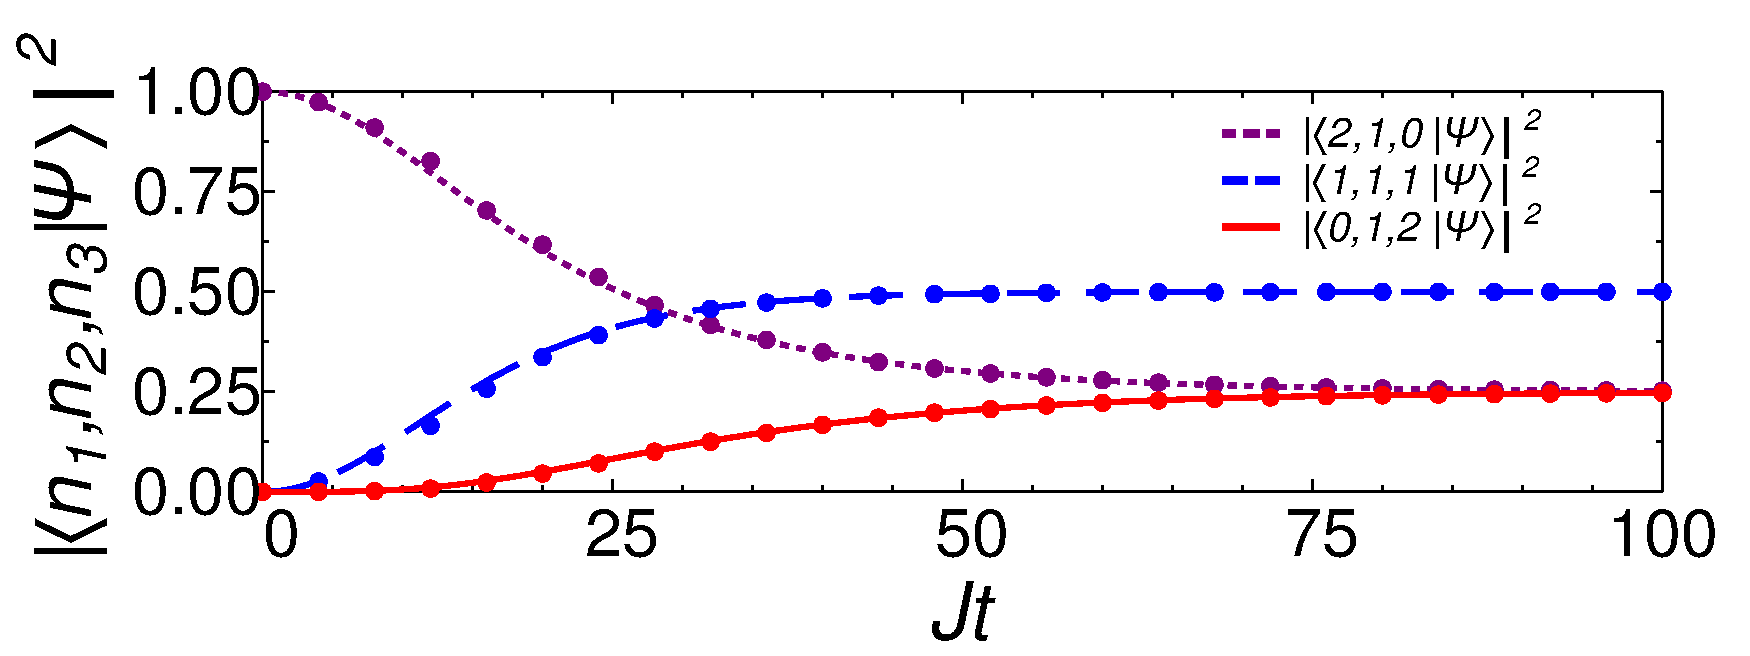
\includegraphics[width=\linewidth]{comp}
	\caption[Fock State Populations in a Zeno
        Subspace]{Populations of the Fock states in the Zeno subspace
          for $\gamma/J = 100$ and initial state $| 2,1,0 \rangle$. It
          is clear that quantum Zeno dynamics occurs via Raman-like
          processes even though none of these states are connected in
          $\hat{H}_0$. The dynamics occurs via virtual intermediate
          states outside the Zeno subspace. The system also tends to a
          steady state which minimises tunnelling effectively
          suppressing fluctuations. The lines are solutions to the
          non-Hermitian Hamiltonian, and the dots are points from a
          stochastic trajectory calculation.\label{fig:comp}}
\end{figure}

\subsection{Steady State of non-Hermitian Dynamics}

A distinctive difference between Bose-Hubbard model ground states and
the final steady state,
$| \Psi \rangle = [|2,1,0 \rangle - \sqrt{2} |1,1,1\rangle +
|0,1,2\rangle]/2$, is that its components are not in phase. Squeezing
due to measurement naturally competes with inter-site tunnelling which
tends to spread the atoms. However, from Eq. \eqref{eq:nHH2} we see
the final state will always be the eigenvector with the smallest
fluctuations as it will have an eigenvalue with the largest imaginary
component. This naturally corresponds to the state where tunnelling
between Zeno subspaces (here between every site) is minimised by
destructive matter-wave interference, i.e.~the tunnelling dark state
defined by $\hat{T} |\Psi \rangle = 0$, where
$\hat{T} = \sum_{\langle i, j \rangle} \bd_i b_j$. This is simply the
physical interpretation of the steady states we predicted for
Eq. \eqref{eq:master}. Crucially, this state can only be reached if
the dynamics aren't fully suppressed by measurement and thus,
counter-intuitively, the atomic dynamics cooperate with measurement to
suppress itself by destructive interference. Therefore, this effect is
beyond the scope of traditional quantum Zeno dynamics and presents a
new perspective on the competition between a system's short-range
dynamics and global measurement backaction.

We now consider a one-dimensional lattice with $M$ sites so we extend
the measurement to $\hat{D} = \N_\text{even}$ where every even site is
illuminated.  The wavefunction in a Zeno subspace must be an
eigenstate of $\c$ and we combine this with the requirement for it to
be in the dark state of the tunnelling operator (eigenstate of $\H_0$
for $U = 0$) to derive the steady state. These two conditions in
momentum space are
\begin{equation}
  \hat{T} | \Psi \rangle = \sum_{\text{RBZ}} \left[ \bd_k b_k -
    \bd_{q} b_{q} \right] \cos(ka) |\Psi \rangle = 0, \nonumber
\end{equation}
\begin{equation}
  \Delta \N |\Psi \rangle = \sum_{\text{RBZ}} \left[ \bd_k b_{-q} +
    \bd_{-q} b_k \right] | \Psi \rangle= \Delta N |\Psi \rangle, \nonumber
\end{equation}
where $b_k = \frac{1}{\sqrt{M}} \sum_j e^{i k j a} b_j$,
$\Delta \hat{N} = \hat{D} - N/2$, $q = \pi/a - k$, $a$ is the lattice
spacing, $N$ the total atom number, and we perform summations over the
reduced Brillouin zone (RBZ), $-\pi/2a < k \le \pi/2a$, as the
symmetries of the system are clearer this way. Now we define
\begin{equation}
\hat{\alpha}_k^\dagger = \bd_k \bd_q - \bd_{-k} \bd_{-q},
\end{equation}
\begin{equation}
\hat{\beta}_\varphi^\dagger = \bd_{\pi/2a} + \varphi \bd_{-\pi/2a},
\end{equation}
where $\varphi = \Delta N / | \Delta N |$, which create the smallest
possible states that satisfy the two equations for $\Delta N = 0$ and
$\Delta N \ne 0$ respectively. Therefore, by noting that
\begin{align}
  \left[ \hat{T}, \hat{\alpha}_k^\dagger \right] & = 0, \\
  \left[ \hat{T}, \hat{\beta}_\varphi^\dagger \right] & = 0, \\
  \left[ \Delta \N, \hat{\alpha}_k^\dagger \right] & = 0, \\
  \left[ \Delta \N, \hat{\beta}_\varphi^\dagger \right] & = \varphi
  \hat{\beta}_\varphi^\dagger,
\end{align}
we can now write the equation for the $N$-particle steady state
\begin{equation}
  \label{eq:ss}
  | \Psi \rangle \propto \left[ \prod_{i=1}^{(N - |\Delta N|)/2}
    \left( \sum_{k = 0}^{\pi/2a} \phi_{i,k} \hat{\alpha}_k^\dagger
    \right) \right] \left( \hat{\beta}_\varphi^\dagger \right)^{|
    \Delta N |} | 0 \rangle, \nonumber
\end{equation}
where $\phi_{i,k}$ are coefficients that depend on the trajectory
taken to reach this state and $|0 \rangle$ is the vacuum state defined
by $b_k |0 \rangle = 0$. Since this a dark state (an eigenstate of
$\H_0$) of the atomic dynamics, this state will remain stationary even
with measurement switched-off. Interestingly, this state is very
different from the ground states of the Bose-Hubbard Hamiltonian, it
is even orthogonal to the superfluid state, and thus it cannot be
obtained by cooling or projecting from an initial ground state. The
combination of tunnelling with measurement is necessary.

\begin{figure}[hbtp!]
	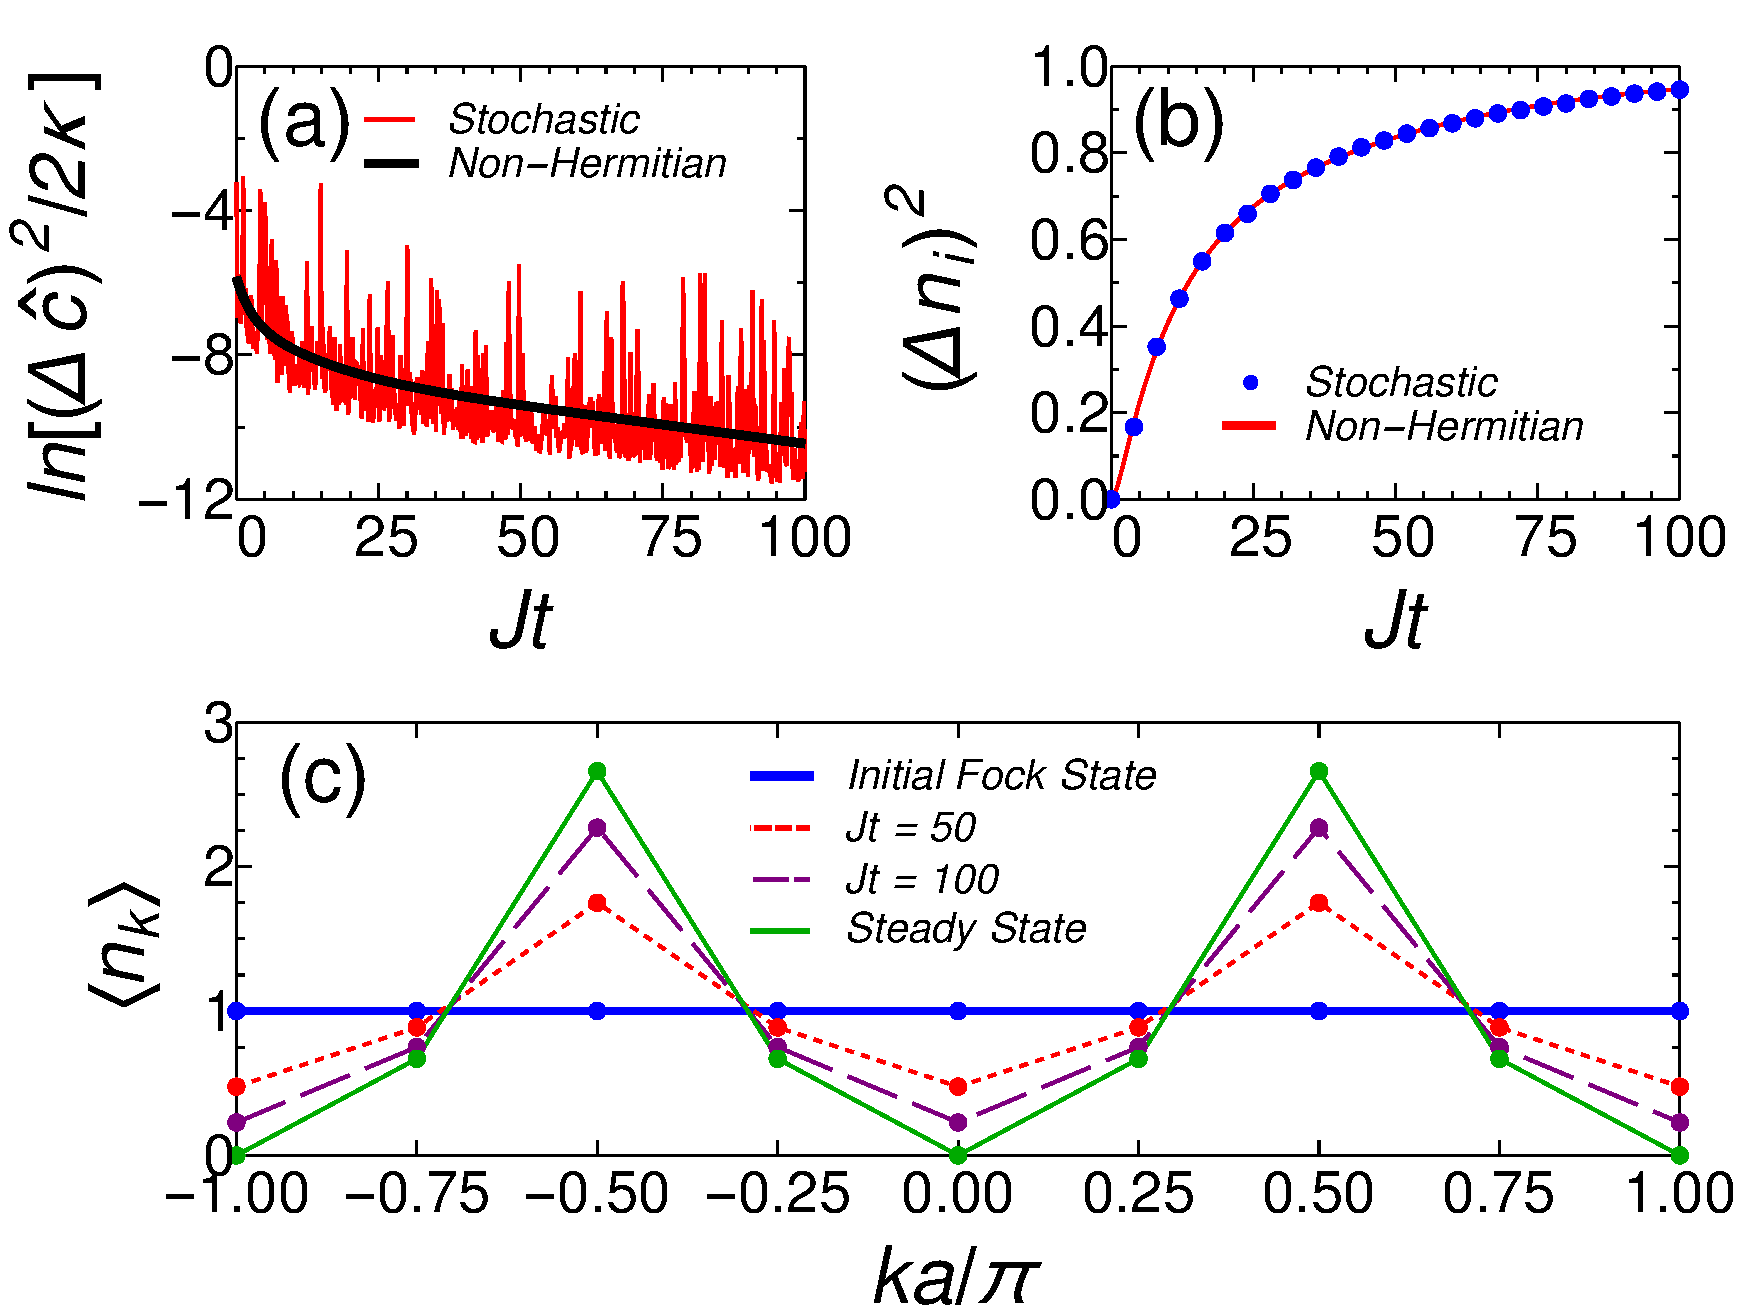
\includegraphics[width=\linewidth]{steady}
	\caption[Non-Hermitian Steady State]{A trajectory simulation
          for eight atoms in eight sites, initially in
          $|1,1,1,1,1,1,1,1 \rangle$, with periodic boundary
          conditions and $\gamma/J = 100$. (a), The fluctuations in
          $\c$ where the stochastic nature of the process is clearly
          visible on a single trajectory level. However, the general
          trend is captured by the non-Hermitian Hamiltonian. (b), The
          local density variance. Whilst the fluctuations in the
          global measurement operator decrease, the fluctuations in
          local density increase due to tunnelling via states outside
          the Zeno subspace. (c), The momentum distribution. The
          initial Fock state has a flat distribution which with time
          approaches the steady state distribution of two identical
          and symmetric distributions centred at $k = \pi/2a$ and
          $k = -\pi/2a$.\label{fig:steady}}
\end{figure}

In order to prepare the steady state one has to run the experiment and
wait until the photocount rate remains constant for a sufficiently
long time. Such a trajectory is illustrated in Fig. \ref{fig:steady}
and compared to a deterministic trajectory calculated using the
non-Hermitian Hamiltonian. It is easy to see from
Fig. \ref{fig:steady}(a) how the stochastic fluctuations around the
mean value of the observable have no effect on the general behaviour
of the system in the strong measurement regime. By discarding these
fluctuations we no longer describe a pure state, but we showed how
this only leads to a negligible error. Fig. \ref{fig:steady}(b) shows
the local density variance in the lattice. Not only does it grow
showing evidence of tunnelling between illuminated and non-illuminated
sites, but it grows to significant values. This is in contrast to
conventional quantum Zeno dynamics where no tunnelling would be
allowed at all. Finally, Fig. \ref{fig:steady}(c) shows the momentum
distribution of the trajectory. We can clearly see that it deviates
significantly from the initial flat distribution of the Fock
state. Furthermore, the steady state does not have any atoms in the
$k=0$ state and thus is orthogonal to the superfluid state as
discussed.

To obtain a state with a specific value of $\Delta N$ postselection
may be necessary, but otherwise it is not needed.  The process can be
optimised by feedback control since the state is monitored at all
times \cite{ivanov2014}. Furthermore, the form of the measurement
operator is very flexible and it can easily be engineered by the
geometry of the optical setup \cite{elliott2015, mazzucchi2016} which
can be used to design a state with desired properties.

\section{Conclusions}

In this chapter we have demonstrated that global quantum measurement
backaction can efficiently compete with standard local processes in
many-body systems. This introduces a completely new energy and time
scale into quantum many-body research. This is made possbile by the
ability to structure the spatial profile of the measurement on a
microscopic scale comparable to the lattice period without the need
for single site addressing. The extreme flexibility of the setup
considered allowed us to effectively tailor long-range entanglement
and correlations present in the system. We showed that the competition
between the global backaction and usual atomic dynamics leads to the
production of spatially multimode macroscopic superpositions which
exhibit large-scale oscillatory dynamics which could be used for
quantum information and metrology. We subsequently demonstrated that
when on-site atomic interactions are introduced the dynamics become
much more complicated with different regimes of behaviour where
measurement and interactions can either compete or cooperate. In the
strong measurement regime we showed that conventional quantum Zeno
dynamics can be realised, but more interestingly, by considering a
strong, but not projective, limit of measurement we observe a new type
of nonlocal dynamics. It turns out that a global measurement scheme
leads to correlations between spatially separated tunnelling events
which conserve the Zeno subspace via Raman-like processes which would
be forbidden in the canonical fully projective limit. We subsequently
presented a rigorous analysis of the underlying process of this new
type of quantum Zeno dynamics in which we showed that in this limit
quantum trajectories can be described by a deterministic non-Hermitian
Hamiltonian. In contrast to previous works, it is independent of the
underlying system and there is no need to postselect a particular
exotic trajectory \cite{lee2014prx, lee2014prl}. Finally, we have
shown that the system will always tend towards the eigenstate of the
Hamiltonian with the best squeezing of the observable and the atomic
dynamics, which normally tend to spread the distribution, cooperates
with measurement to produce a state in which tunnelling is suppressed
by destructive matter-wave interference. A dark state of the
tunnelling operator will have zero fluctuations and we provided an
expression for the steady state which is significantly different from
the ground state of the Hamiltonian. This is in contrast to previous
works on dissipative state preparation where the steady state had to
be a dark state of the measurement operator \cite{diehl2008}.

Such globally paired tunnelling due to a fundamentally new phenomenon,
global quantum measurement backaction, can enrich the physics of
long-range correlated systems beyond relatively short-range
interactions expected from standard dipole-dipole interactions
\cite{sowinski2012, omjyoti2015}. These nonlocal high-order processes
entangle regions of the optical lattice that are disconnected by the
measurement. Using different detection schemes, we showed how to
tailor density-density correlations between distant lattice
sites. Quantum optical engineering of nonlocal coupling to
environment, combined with quantum measurement, can allow the design
of nontrivial system-bath interactions, enabling new links to quantum
simulations~\cite{stannigel2013} and thermodynamics~\cite{erez2008}
and extend these directions to the field of non-Hermitian quantum
mechanics, where quantum optical setups are particularly
promising~\cite{lee2014prl}. Importantly, both systems and baths,
designed by our method, can be strongly correlated systems with
internal long-range entanglement.

%%*******************************************************************************
%*********************************** Sixth Chapter *****************************
%*******************************************************************************

\chapter{Phase Measurement Induced Dynamics}
% Title of the Sixth Chapter

\ifpdf
    \graphicspath{{Chapter6/Figs/Raster/}{Chapter6/Figs/PDF/}{Chapter6/Figs/}}
\else
    \graphicspath{{Chapter6/Figs/Vector/}{Chapter6/Figs/}}
\fi


\section{Introduction}

\section{Diffraction Maximum and Energy Eigenstates}

\section{General Model for Weak Measurement Projection}

\section{Determining the Projection Subspace}

\section{Conclusions}
%%*******************************************************************************
%*********************************** Seventh Chapter *****************************
%*******************************************************************************

\chapter{Summary and Conclusions}  %Title of the Seventh Chapter

\ifpdf
    \graphicspath{{Chapter7/Figs/Raster/}{Chapter7/Figs/PDF/}{Chapter7/Figs/}}
\else
    \graphicspath{{Chapter7/Figs/Vector/}{Chapter7/Figs/}}
\fi

Quantum optics of quantum gases explores the ultimate quantum regime
of light-matter interactions where both the optical and matter fields
are fully quantised. It provides a very rich system in which new
phenomena can be observed, engineered, and controlled beyond what
would be possible in condensed matter. Combined with rapid and
promising experimental progress in this field the theoretical
proposals have the potential of directing the research in the
foreseeable future \cite{baumann2010, wolke2012, schmidt2014,
  klinder2015, landig2016}.

In this thesis we focused on the coupling between global quantised
optical fields and an ultracold bosonic quantum gas. By considering
global fields as opposed to localised light-matter interactions we
were able to introduce several nonlocal properties to the Hamiltonian
in a controllable manner which would otherwise be impossible to
implement. We showed how this can be useful in the context of
nondestructive probing by showing that it can easily distinguish
between a highly delocalised quantum state such as a superfluid and
insulating states such as the Mott insulator and the Bose glass phases
which is currently a challenge \cite{derrico2014}. Furthermore, we
have seen how the correlation length, which would be inaccessible in
localised measurements, was immediately visible in our scheme and lead
to an angular scattering pattern that was far richer than it was for
the classical case. This is best highlighted by the fact that it would
be visible even when classically no light would scatter coherently at
all.

More interestingly, the global nature of the measurement was also
capable of creating such long-range correlations itself when we
considered measurement backaction. This was most visible when we saw
how weak measurement was capable of driving global macroscopic
multimode oscillations between different spatial modes, such as odd
and even sites, across the whole lattice which could be used for
quantum information and metrology. Such dynamical states show spatial
density-density correlations with nontrivial periods and long-range
coherence, thus having supersolid properties, but as an essentially
dynamical version. Furthermore, the tunability of the optical
arrangement meant that we had extreme flexibility in choosing our
observables, effectively tailoring the long-range entanglement and
correlations in the system. We have also shown how global measurement
when combined with both atomic tunnelling and interactions leads to
highly nontrivial dynamics in which backaction can either compete or
cooperate with on-site repulsion in squeezing the atomic variables.

In the limit of strong measurement when quantum Zeno dynamics occurs
we showed that these nonlocal spatial modes created by the global
measurement lead to long-range correlated tunnelling events whilst
suppressing any other dynamics between different spatial modes of the
measurement. Such globally paired tunneling due to a fundamentally
novel phenomenon can enrich physics of long-range correlated systems
beyond relatively shortrange interactions expected from standard
dipole-dipole interactions \cite{sowinski2012, omjyoti2015}. These
nonlocal high-order processes entangle regions of the optical lattice
that are disconnected by the measurement. Using different detection
schemes, we showed how to tailor density-density correlations between
distant lattice sites. Quantum optical engineering of nonlocal
coupling to environment, combined with quantum measurement, can allow
the design of nontrivial system-bath interactions, enabling new links
to quantum simulations \cite{stannigel2013} and thermodynamics
\cite{erez2008}. Interestingly, these dynamics also provide a link to
non-Hermitian quantum mechanics as this regime of measurement can be
accurately described with a non-Hermitian Hamiltonian. Furthermore, we
show that this allows for a rather novel type of competition between
measurement and tunnelling where both processes actually cooperate to
produce a steady state in which tunnelling is suppressed by
destructive matter-wave interference.

A unique feature of our global measurement scheme meant that we could
couple directly to the phase observables of the system by coupling to
the interference between the lattice sites, which represents the
shortest meaningful distance in an optical lattice, rather than their
on-site density. This defines most processes in optical lattices.  For
example, matter-field phase changes may happen not only due to
external gradients, but also due to intriguing effects such quantum
jumps leading to phase flips at neighbouring sites and sudden
cancellation of tunneling \cite{vukics2007}, which should be
accessible by this method. Furthremore, in mean-field one can measure
the matter-field amplitude (which is also the order parameter),
quadratures and their squeezing. This can link atom optics to areas
where quantum optics has already made progress, e.g., quantum imaging
\cite{golubev2010, kolobov1999}, using an optical lattice as an array
of multimode nonclassical matter- field sources with a high degree of
entanglement for quantum information processing. We have also shown
how this scheme of coupling to phase observables can be used in the
context of quantum measurement backaction to achieve a new degree of
control. We used this result to show a generalisation of weak
measurement on dynamical systems by showing that there is now a new
class of projections available even when the measurement is not a
compatible observable of the Hamiltonian. This an interesting result
as the projections themselves are unlike those postulated by the
Copenhagen interpretation, those present in quantum Zeno dynamic, or
even those possible to engineer using dissipative methods.

In this thesis we have covered significant areas of the broad field
that is quantum optics of quantum gases, but there is much more that
has been left untouched. Here, we have only considered spinless
bosons, but the theory can also been extended to fermions
\cite{atoms2015, mazzucchi2016, mazzucchi2016af} and molecules
\cite{LP2013} and potentially even photonic circuits
\cite{mazzucchi2016njp}. Furthermore, the question of quantum
measurement and its properties has been a subject of heated debate
since the very origins of quantum theory yet it is still as mysterious
as it was at the beginning of the $20^\mathrm{th}$ century. However,
this work has hopefully demonstrated that coupling quantised light
fields to many-body systems provides a very rich playground for
exploring new quantum mechanical phenomena especially the competition
between weak quantum measurement and many-body dynamics in ultracold
bosonic gases.




% ********************************** Back Matter *******************************
% Backmatter should be commented out, if you are using appendices after References
%\backmatter

% ********************************** Bibliography ******************************
\begin{spacing}{0.9}

% To use the conventional natbib style referencing
% Bibliography style previews: http://nodonn.tipido.net/bibstyle.php
% Reference styles: http://sites.stat.psu.edu/~surajit/present/bib.htm

%\bibliographystyle{apalike}
\bibliographystyle{unsrt} % Use for unsorted references  
%\bibliographystyle{plainnat} % use this to have URLs listed in References
\cleardoublepage
\bibliography{References/references} % Path to your References.bib file


% If you would like to use BibLaTeX for your references, pass `custombib' as
% an option in the document class. The location of 'reference.bib' should be
% specified in the preamble.tex file in the custombib section.
% Comment out the lines related to natbib above and uncomment the following line.

%\printbibliography[heading=bibintoc, title={References}]


\end{spacing}

% ********************************** Appendices ********************************

%\begin{appendices} % Using appendices environment for more functunality

%% ******************************* Thesis Appendix A ****************************
\chapter{How to install \LaTeX} 

\section*{Windows OS}

\subsection*{TeXLive package - full version}
\begin{enumerate}
\item	Download the TeXLive ISO (2.2GB) from\\
\href{https://www.tug.org/texlive/}{https://www.tug.org/texlive/}
\item	Download WinCDEmu (if you don't have a virtual drive) from \\
\href{http://wincdemu.sysprogs.org/download/}
{http://wincdemu.sysprogs.org/download/}
\item	To install Windows CD Emulator follow the instructions at\\
\href{http://wincdemu.sysprogs.org/tutorials/install/}
{http://wincdemu.sysprogs.org/tutorials/install/}
\item	Right click the iso and mount it using the WinCDEmu as shown in \\
\href{http://wincdemu.sysprogs.org/tutorials/mount/}{
http://wincdemu.sysprogs.org/tutorials/mount/}
\item	Open your virtual drive and run setup.pl
\end{enumerate}

or

\subsection*{Basic MikTeX - \TeX~ distribution}
\begin{enumerate}
\item	Download Basic-MiK\TeX (32bit or 64bit) from\\
\href{http://miktex.org/download}{http://miktex.org/download}
\item	Run the installer 
\item	To add a new package go to Start >> All Programs >> MikTex >> Maintenance (Admin) and choose Package Manager
\item	Select or search for packages to install
\end{enumerate}

\subsection*{TexStudio - \TeX~ editor}
\begin{enumerate}
\item	Download TexStudio from\\
\href{http://texstudio.sourceforge.net/\#downloads}
{http://texstudio.sourceforge.net/\#downloads} 
\item	Run the installer
\end{enumerate}

\section*{Mac OS X}
\subsection*{MacTeX - \TeX~ distribution}
\begin{enumerate}
\item	Download the file from\\
\href{https://www.tug.org/mactex/}{https://www.tug.org/mactex/}
\item	Extract and double click to run the installer. It does the entire configuration, sit back and relax.
\end{enumerate}

\subsection*{TexStudio - \TeX~ editor}
\begin{enumerate}
\item	Download TexStudio from\\
\href{http://texstudio.sourceforge.net/\#downloads}
{http://texstudio.sourceforge.net/\#downloads} 
\item	Extract and Start
\end{enumerate}


\section*{Unix/Linux}
\subsection*{TeXLive - \TeX~ distribution}
\subsubsection*{Getting the distribution:}
\begin{enumerate}
\item	TexLive can be downloaded from\\
\href{http://www.tug.org/texlive/acquire-netinstall.html}
{http://www.tug.org/texlive/acquire-netinstall.html}.
\item	TexLive is provided by most operating system you can use (rpm,apt-get or yum) to get TexLive distributions
\end{enumerate}

\subsubsection*{Installation}
\begin{enumerate}
\item	Mount the ISO file in the mnt directory
\begin{verbatim}
mount -t iso9660 -o ro,loop,noauto /your/texlive####.iso /mnt
\end{verbatim}

\item	Install wget on your OS (use rpm, apt-get or yum install)
\item	Run the installer script install-tl.
\begin{verbatim}
	cd /your/download/directory
	./install-tl
\end{verbatim}
\item	Enter command `i' for installation

\item	Post-Installation configuration:\\
\href{http://www.tug.org/texlive/doc/texlive-en/texlive-en.html\#x1-320003.4.1}
{http://www.tug.org/texlive/doc/texlive-en/texlive-en.html\#x1-320003.4.1} 
\item	Set the path for the directory of TexLive binaries in your .bashrc file
\end{enumerate}

\subsubsection*{For 32bit OS}
For Bourne-compatible shells such as bash, and using Intel x86 GNU/Linux and a default directory setup as an example, the file to edit might be \begin{verbatim}
edit $~/.bashrc file and add following lines
PATH=/usr/local/texlive/2011/bin/i386-linux:$PATH; 
export PATH 
MANPATH=/usr/local/texlive/2011/texmf/doc/man:$MANPATH;
export MANPATH 
INFOPATH=/usr/local/texlive/2011/texmf/doc/info:$INFOPATH;
export INFOPATH
\end{verbatim}
\subsubsection*{For 64bit OS}
\begin{verbatim}
edit $~/.bashrc file and add following lines
PATH=/usr/local/texlive/2011/bin/x86_64-linux:$PATH;
export PATH 
MANPATH=/usr/local/texlive/2011/texmf/doc/man:$MANPATH;
export MANPATH 
INFOPATH=/usr/local/texlive/2011/texmf/doc/info:$INFOPATH;
export INFOPATH

\end{verbatim}



%\subsection{Installing directly using Linux packages} 
\subsubsection*{Fedora/RedHat/CentOS:}
\begin{verbatim} 
sudo yum install texlive 
sudo yum install psutils 
\end{verbatim}


\subsubsection*{SUSE:}
\begin{verbatim}
sudo zypper install texlive
\end{verbatim}


\subsubsection*{Debian/Ubuntu:}
\begin{verbatim} 
sudo apt-get install texlive texlive-latex-extra 
sudo apt-get install psutils
\end{verbatim}

%% ******************************* Thesis Appendix B ********************************

\chapter{Installing the CUED class file}

\LaTeX.cls files can be accessed system-wide when they are placed in the
<texmf>/tex/latex directory, where <texmf> is the root directory of the user’s \TeX installation. On systems that have a local texmf tree (<texmflocal>), which
may be named ``texmf-local'' or ``localtexmf'', it may be advisable to install packages in <texmflocal>, rather than <texmf> as the contents of the former, unlike that of the latter, are preserved after the \LaTeX system is reinstalled and/or upgraded.

It is recommended that the user create a subdirectory <texmf>/tex/latex/CUED for all CUED related \LaTeX class and package files. On some \LaTeX systems, the directory look-up tables will need to be refreshed after making additions or deletions to the system files. For \TeX Live systems this is accomplished via executing ``texhash'' as root. MIK\TeX users can run ``initexmf -u'' to accomplish the same thing.

Users not willing or able to install the files system-wide can install them in their personal directories, but will then have to provide the path (full or relative) in addition to the filename when referring to them in \LaTeX.



%\end{appendices}

% *************************************** Index ********************************
\printthesisindex % If index is present

\end{document}
